\documentclass[twoside]{book}

% Packages required by doxygen
\usepackage{fixltx2e}
\usepackage{calc}
\usepackage{doxygen}
\usepackage[export]{adjustbox} % also loads graphicx
\usepackage{graphicx}
\usepackage[utf8]{inputenc}
\usepackage{makeidx}
\usepackage{multicol}
\usepackage{multirow}
\PassOptionsToPackage{warn}{textcomp}
\usepackage{textcomp}
\usepackage[nointegrals]{wasysym}
\usepackage[table]{xcolor}

% Font selection
\usepackage[T1]{fontenc}
\usepackage[scaled=.90]{helvet}
\usepackage{courier}
\usepackage{amssymb}
\usepackage{sectsty}
\renewcommand{\familydefault}{\sfdefault}
\allsectionsfont{%
  \fontseries{bc}\selectfont%
  \color{darkgray}%
}
\renewcommand{\DoxyLabelFont}{%
  \fontseries{bc}\selectfont%
  \color{darkgray}%
}
\newcommand{\+}{\discretionary{\mbox{\scriptsize$\hookleftarrow$}}{}{}}

% Page & text layout
\usepackage{geometry}
\geometry{%
  a4paper,%
  top=2.5cm,%
  bottom=2.5cm,%
  left=2.5cm,%
  right=2.5cm%
}
\tolerance=750
\hfuzz=15pt
\hbadness=750
\setlength{\emergencystretch}{15pt}
\setlength{\parindent}{0cm}
\setlength{\parskip}{3ex plus 2ex minus 2ex}
\makeatletter
\renewcommand{\paragraph}{%
  \@startsection{paragraph}{4}{0ex}{-1.0ex}{1.0ex}{%
    \normalfont\normalsize\bfseries\SS@parafont%
  }%
}
\renewcommand{\subparagraph}{%
  \@startsection{subparagraph}{5}{0ex}{-1.0ex}{1.0ex}{%
    \normalfont\normalsize\bfseries\SS@subparafont%
  }%
}
\makeatother

% Headers & footers
\usepackage{fancyhdr}
\pagestyle{fancyplain}
\fancyhead[LE]{\fancyplain{}{\bfseries\thepage}}
\fancyhead[CE]{\fancyplain{}{}}
\fancyhead[RE]{\fancyplain{}{\bfseries\leftmark}}
\fancyhead[LO]{\fancyplain{}{\bfseries\rightmark}}
\fancyhead[CO]{\fancyplain{}{}}
\fancyhead[RO]{\fancyplain{}{\bfseries\thepage}}
\fancyfoot[LE]{\fancyplain{}{}}
\fancyfoot[CE]{\fancyplain{}{}}
\fancyfoot[RE]{\fancyplain{}{\bfseries\scriptsize Generated by Doxygen }}
\fancyfoot[LO]{\fancyplain{}{\bfseries\scriptsize Generated by Doxygen }}
\fancyfoot[CO]{\fancyplain{}{}}
\fancyfoot[RO]{\fancyplain{}{}}
\renewcommand{\footrulewidth}{0.4pt}
\renewcommand{\chaptermark}[1]{%
  \markboth{#1}{}%
}
\renewcommand{\sectionmark}[1]{%
  \markright{\thesection\ #1}%
}

% Indices & bibliography
\usepackage{natbib}
\usepackage[titles]{tocloft}
\setcounter{tocdepth}{3}
\setcounter{secnumdepth}{5}
\makeindex

% Hyperlinks (required, but should be loaded last)
\usepackage{ifpdf}
\ifpdf
  \usepackage[pdftex,pagebackref=true]{hyperref}
\else
  \usepackage[ps2pdf,pagebackref=true]{hyperref}
\fi
\hypersetup{%
  colorlinks=true,%
  linkcolor=blue,%
  citecolor=blue,%
  unicode%
}

% Custom commands
\newcommand{\clearemptydoublepage}{%
  \newpage{\pagestyle{empty}\cleardoublepage}%
}

\usepackage{caption}
\captionsetup{labelsep=space,justification=centering,font={bf},singlelinecheck=off,skip=4pt,position=top}

%===== C O N T E N T S =====

\begin{document}

% Titlepage & ToC
\hypersetup{pageanchor=false,
             bookmarksnumbered=true,
             pdfencoding=unicode
            }
\pagenumbering{alph}
\begin{titlepage}
\vspace*{7cm}
\begin{center}%
{\Large Train-\/\+System }\\
\vspace*{1cm}
{\large Generated by Doxygen 1.8.14}\\
\end{center}
\end{titlepage}
\clearemptydoublepage
\pagenumbering{roman}
\tableofcontents
\clearemptydoublepage
\pagenumbering{arabic}
\hypersetup{pageanchor=true}

%--- Begin generated contents ---
\chapter{Namespace Index}
\section{Namespace List}
Here is a list of all namespaces with brief descriptions\+:\begin{DoxyCompactList}
\item\contentsline{section}{\mbox{\hyperlink{namespaceproject__utils}{project\+\_\+utils}} }{\pageref{namespaceproject__utils}}{}
\end{DoxyCompactList}

\chapter{Hierarchical Index}
\section{Class Hierarchy}
This inheritance list is sorted roughly, but not completely, alphabetically\+:\begin{DoxyCompactList}
\item \contentsline{section}{Date}{\pageref{classDate}}{}
\item \contentsline{section}{Engineer\+:\+:Engineer\+Hash\+Utils}{\pageref{structEngineer_1_1EngineerHashUtils}}{}
\item exception\begin{DoxyCompactList}
\item \contentsline{section}{Identical\+Destination\+Exception}{\pageref{classIdenticalDestinationException}}{}
\item \contentsline{section}{Invalid\+Date\+Exception}{\pageref{classInvalidDateException}}{}
\item \contentsline{section}{Invalid\+Train\+Type\+Exception}{\pageref{classInvalidTrainTypeException}}{}
\item \contentsline{section}{No\+Such\+Engineer\+Exception}{\pageref{classNoSuchEngineerException}}{}
\item \contentsline{section}{No\+Such\+Passenger\+Exception}{\pageref{classNoSuchPassengerException}}{}
\item \contentsline{section}{No\+Such\+Station\+Exception}{\pageref{classNoSuchStationException}}{}
\item \contentsline{section}{No\+Such\+Train\+Exception}{\pageref{classNoSuchTrainException}}{}
\item \contentsline{section}{No\+Such\+Trip\+Exception}{\pageref{classNoSuchTripException}}{}
\item \contentsline{section}{Reverse\+Dates\+Exception}{\pageref{classReverseDatesException}}{}
\item \contentsline{section}{Trip\+Past\+Exception}{\pageref{classTripPastException}}{}
\end{DoxyCompactList}
\item \contentsline{section}{Passenger\+Card}{\pageref{classPassengerCard}}{}
\item \contentsline{section}{Purchase\+Log}{\pageref{classPurchaseLog}}{}
\item \contentsline{section}{Repair\+Shop\+:\+:Repair\+Shop\+P\+Q\+Utils}{\pageref{structRepairShop_1_1RepairShopPQUtils}}{}
\item \contentsline{section}{System}{\pageref{classSystem}}{}
\item \contentsline{section}{System\+Element}{\pageref{classSystemElement}}{}
\begin{DoxyCompactList}
\item \contentsline{section}{Person}{\pageref{classPerson}}{}
\begin{DoxyCompactList}
\item \contentsline{section}{Engineer}{\pageref{classEngineer}}{}
\item \contentsline{section}{Passenger}{\pageref{classPassenger}}{}
\end{DoxyCompactList}
\item \contentsline{section}{Repair\+Shop}{\pageref{classRepairShop}}{}
\item \contentsline{section}{Station}{\pageref{classStation}}{}
\item \contentsline{section}{Train}{\pageref{classTrain}}{}
\begin{DoxyCompactList}
\item \contentsline{section}{Alfa\+Pendular}{\pageref{classAlfaPendular}}{}
\item \contentsline{section}{Inter\+Cidades}{\pageref{classInterCidades}}{}
\end{DoxyCompactList}
\item \contentsline{section}{Trip}{\pageref{classTrip}}{}
\end{DoxyCompactList}
\item \contentsline{section}{Ticket\+Invoice}{\pageref{classTicketInvoice}}{}
\item \contentsline{section}{Ticket\+Purchase\+Request}{\pageref{classTicketPurchaseRequest}}{}
\end{DoxyCompactList}

\chapter{Class Index}
\section{Class List}
Here are the classes, structs, unions and interfaces with brief descriptions\+:\begin{DoxyCompactList}
\item\contentsline{section}{\mbox{\hyperlink{classDate}{Date}} \\*Class for representing dates in the program }{\pageref{classDate}}{}
\item\contentsline{section}{\mbox{\hyperlink{classPassenger}{Passenger}} \\*Class for representing a passenger in the system }{\pageref{classPassenger}}{}
\item\contentsline{section}{\mbox{\hyperlink{classPassengerCard}{Passenger\+Card}} \\*Class for representing the card of a passenger in the system }{\pageref{classPassengerCard}}{}
\item\contentsline{section}{\mbox{\hyperlink{classPurchaseLog}{Purchase\+Log}} }{\pageref{classPurchaseLog}}{}
\item\contentsline{section}{\mbox{\hyperlink{classStation}{Station}} \\*Class for representing a station in the system }{\pageref{classStation}}{}
\item\contentsline{section}{\mbox{\hyperlink{classSystem}{System}} \\*Class to represent the central system }{\pageref{classSystem}}{}
\item\contentsline{section}{\mbox{\hyperlink{classTicketInvoice}{Ticket\+Invoice}} \\*Class for representing an invoice of a ticket purchase in the system }{\pageref{classTicketInvoice}}{}
\item\contentsline{section}{\mbox{\hyperlink{classTicketPurchaseRequest}{Ticket\+Purchase\+Request}} \\*Class to represent a ticket purchase request }{\pageref{classTicketPurchaseRequest}}{}
\item\contentsline{section}{\mbox{\hyperlink{classTrain}{Train}} \\*Class for representing a train in the system }{\pageref{classTrain}}{}
\item\contentsline{section}{\mbox{\hyperlink{classTrip}{Trip}} \\*Class for representing a trip in the system }{\pageref{classTrip}}{}
\end{DoxyCompactList}

\chapter{File Index}
\section{File List}
Here is a list of all files with brief descriptions\+:\begin{DoxyCompactList}
\item\contentsline{section}{\mbox{\hyperlink{Date_8cpp}{Date.\+cpp}} }{\pageref{Date_8cpp}}{}
\item\contentsline{section}{\mbox{\hyperlink{Date_8h}{Date.\+h}} }{\pageref{Date_8h}}{}
\item\contentsline{section}{\mbox{\hyperlink{project__utils_8cpp}{project\+\_\+utils.\+cpp}} }{\pageref{project__utils_8cpp}}{}
\item\contentsline{section}{\mbox{\hyperlink{project__utils_8h}{project\+\_\+utils.\+h}} }{\pageref{project__utils_8h}}{}
\item\contentsline{section}{\mbox{\hyperlink{PurchaseLog_8cpp}{Purchase\+Log.\+cpp}} }{\pageref{PurchaseLog_8cpp}}{}
\item\contentsline{section}{\mbox{\hyperlink{PurchaseLog_8h}{Purchase\+Log.\+h}} }{\pageref{PurchaseLog_8h}}{}
\item\contentsline{section}{\mbox{\hyperlink{System_8cpp}{System.\+cpp}} }{\pageref{System_8cpp}}{}
\item\contentsline{section}{\mbox{\hyperlink{System_8h}{System.\+h}} }{\pageref{System_8h}}{}
\item\contentsline{section}{\mbox{\hyperlink{TicketInvoice_8cpp}{Ticket\+Invoice.\+cpp}} }{\pageref{TicketInvoice_8cpp}}{}
\item\contentsline{section}{\mbox{\hyperlink{TicketInvoice_8h}{Ticket\+Invoice.\+h}} }{\pageref{TicketInvoice_8h}}{}
\item\contentsline{section}{\mbox{\hyperlink{TicketPurchaseRequest_8cpp}{Ticket\+Purchase\+Request.\+cpp}} }{\pageref{TicketPurchaseRequest_8cpp}}{}
\item\contentsline{section}{\mbox{\hyperlink{TicketPurchaseRequest_8h}{Ticket\+Purchase\+Request.\+h}} }{\pageref{TicketPurchaseRequest_8h}}{}
\item\contentsline{section}{\mbox{\hyperlink{Train-System_8cpp}{Train-\/\+System.\+cpp}} }{\pageref{Train-System_8cpp}}{}
\item\contentsline{section}{exceptions/\mbox{\hyperlink{IdenticalDestinationException_8cpp}{Identical\+Destination\+Exception.\+cpp}} }{\pageref{IdenticalDestinationException_8cpp}}{}
\item\contentsline{section}{exceptions/\mbox{\hyperlink{IdenticalDestinationException_8h}{Identical\+Destination\+Exception.\+h}} }{\pageref{IdenticalDestinationException_8h}}{}
\item\contentsline{section}{exceptions/\mbox{\hyperlink{InvalidDateException_8cpp}{Invalid\+Date\+Exception.\+cpp}} }{\pageref{InvalidDateException_8cpp}}{}
\item\contentsline{section}{exceptions/\mbox{\hyperlink{InvalidDateException_8h}{Invalid\+Date\+Exception.\+h}} }{\pageref{InvalidDateException_8h}}{}
\item\contentsline{section}{exceptions/\mbox{\hyperlink{InvalidTrainTypeException_8cpp}{Invalid\+Train\+Type\+Exception.\+cpp}} }{\pageref{InvalidTrainTypeException_8cpp}}{}
\item\contentsline{section}{exceptions/\mbox{\hyperlink{InvalidTrainTypeException_8h}{Invalid\+Train\+Type\+Exception.\+h}} }{\pageref{InvalidTrainTypeException_8h}}{}
\item\contentsline{section}{exceptions/\mbox{\hyperlink{NoSuchEngineerException_8cpp}{No\+Such\+Engineer\+Exception.\+cpp}} }{\pageref{NoSuchEngineerException_8cpp}}{}
\item\contentsline{section}{exceptions/\mbox{\hyperlink{NoSuchEngineerException_8h}{No\+Such\+Engineer\+Exception.\+h}} }{\pageref{NoSuchEngineerException_8h}}{}
\item\contentsline{section}{exceptions/\mbox{\hyperlink{NoSuchPassengerException_8cpp}{No\+Such\+Passenger\+Exception.\+cpp}} }{\pageref{NoSuchPassengerException_8cpp}}{}
\item\contentsline{section}{exceptions/\mbox{\hyperlink{NoSuchPassengerException_8h}{No\+Such\+Passenger\+Exception.\+h}} }{\pageref{NoSuchPassengerException_8h}}{}
\item\contentsline{section}{exceptions/\mbox{\hyperlink{NoSuchStationException_8cpp}{No\+Such\+Station\+Exception.\+cpp}} }{\pageref{NoSuchStationException_8cpp}}{}
\item\contentsline{section}{exceptions/\mbox{\hyperlink{NoSuchStationException_8h}{No\+Such\+Station\+Exception.\+h}} }{\pageref{NoSuchStationException_8h}}{}
\item\contentsline{section}{exceptions/\mbox{\hyperlink{NoSuchTrainException_8cpp}{No\+Such\+Train\+Exception.\+cpp}} }{\pageref{NoSuchTrainException_8cpp}}{}
\item\contentsline{section}{exceptions/\mbox{\hyperlink{NoSuchTrainException_8h}{No\+Such\+Train\+Exception.\+h}} }{\pageref{NoSuchTrainException_8h}}{}
\item\contentsline{section}{exceptions/\mbox{\hyperlink{NoSuchTripException_8cpp}{No\+Such\+Trip\+Exception.\+cpp}} }{\pageref{NoSuchTripException_8cpp}}{}
\item\contentsline{section}{exceptions/\mbox{\hyperlink{NoSuchTripException_8h}{No\+Such\+Trip\+Exception.\+h}} }{\pageref{NoSuchTripException_8h}}{}
\item\contentsline{section}{exceptions/\mbox{\hyperlink{ReverseDatesException_8cpp}{Reverse\+Dates\+Exception.\+cpp}} }{\pageref{ReverseDatesException_8cpp}}{}
\item\contentsline{section}{exceptions/\mbox{\hyperlink{ReverseDatesException_8h}{Reverse\+Dates\+Exception.\+h}} }{\pageref{ReverseDatesException_8h}}{}
\item\contentsline{section}{exceptions/\mbox{\hyperlink{TripPastException_8cpp}{Trip\+Past\+Exception.\+cpp}} }{\pageref{TripPastException_8cpp}}{}
\item\contentsline{section}{exceptions/\mbox{\hyperlink{TripPastException_8h}{Trip\+Past\+Exception.\+h}} }{\pageref{TripPastException_8h}}{}
\item\contentsline{section}{system\+\_\+elements/\mbox{\hyperlink{AlfaPendular_8cpp}{Alfa\+Pendular.\+cpp}} }{\pageref{AlfaPendular_8cpp}}{}
\item\contentsline{section}{system\+\_\+elements/\mbox{\hyperlink{AlfaPendular_8h}{Alfa\+Pendular.\+h}} }{\pageref{AlfaPendular_8h}}{}
\item\contentsline{section}{system\+\_\+elements/\mbox{\hyperlink{Engineer_8cpp}{Engineer.\+cpp}} }{\pageref{Engineer_8cpp}}{}
\item\contentsline{section}{system\+\_\+elements/\mbox{\hyperlink{Engineer_8h}{Engineer.\+h}} }{\pageref{Engineer_8h}}{}
\item\contentsline{section}{system\+\_\+elements/\mbox{\hyperlink{InterCidades_8cpp}{Inter\+Cidades.\+cpp}} }{\pageref{InterCidades_8cpp}}{}
\item\contentsline{section}{system\+\_\+elements/\mbox{\hyperlink{InterCidades_8h}{Inter\+Cidades.\+h}} }{\pageref{InterCidades_8h}}{}
\item\contentsline{section}{system\+\_\+elements/\mbox{\hyperlink{Passenger_8cpp}{Passenger.\+cpp}} }{\pageref{Passenger_8cpp}}{}
\item\contentsline{section}{system\+\_\+elements/\mbox{\hyperlink{Passenger_8h}{Passenger.\+h}} }{\pageref{Passenger_8h}}{}
\item\contentsline{section}{system\+\_\+elements/\mbox{\hyperlink{PassengerCard_8cpp}{Passenger\+Card.\+cpp}} }{\pageref{PassengerCard_8cpp}}{}
\item\contentsline{section}{system\+\_\+elements/\mbox{\hyperlink{PassengerCard_8h}{Passenger\+Card.\+h}} }{\pageref{PassengerCard_8h}}{}
\item\contentsline{section}{system\+\_\+elements/\mbox{\hyperlink{Person_8cpp}{Person.\+cpp}} }{\pageref{Person_8cpp}}{}
\item\contentsline{section}{system\+\_\+elements/\mbox{\hyperlink{Person_8h}{Person.\+h}} }{\pageref{Person_8h}}{}
\item\contentsline{section}{system\+\_\+elements/\mbox{\hyperlink{RepairShop_8cpp}{Repair\+Shop.\+cpp}} }{\pageref{RepairShop_8cpp}}{}
\item\contentsline{section}{system\+\_\+elements/\mbox{\hyperlink{RepairShop_8h}{Repair\+Shop.\+h}} }{\pageref{RepairShop_8h}}{}
\item\contentsline{section}{system\+\_\+elements/\mbox{\hyperlink{Station_8cpp}{Station.\+cpp}} }{\pageref{Station_8cpp}}{}
\item\contentsline{section}{system\+\_\+elements/\mbox{\hyperlink{Station_8h}{Station.\+h}} }{\pageref{Station_8h}}{}
\item\contentsline{section}{system\+\_\+elements/\mbox{\hyperlink{SystemElement_8cpp}{System\+Element.\+cpp}} }{\pageref{SystemElement_8cpp}}{}
\item\contentsline{section}{system\+\_\+elements/\mbox{\hyperlink{SystemElement_8h}{System\+Element.\+h}} }{\pageref{SystemElement_8h}}{}
\item\contentsline{section}{system\+\_\+elements/\mbox{\hyperlink{Train_8cpp}{Train.\+cpp}} }{\pageref{Train_8cpp}}{}
\item\contentsline{section}{system\+\_\+elements/\mbox{\hyperlink{Train_8h}{Train.\+h}} }{\pageref{Train_8h}}{}
\item\contentsline{section}{system\+\_\+elements/\mbox{\hyperlink{Trip_8cpp}{Trip.\+cpp}} }{\pageref{Trip_8cpp}}{}
\item\contentsline{section}{system\+\_\+elements/\mbox{\hyperlink{Trip_8h}{Trip.\+h}} }{\pageref{Trip_8h}}{}
\end{DoxyCompactList}

\chapter{Namespace Documentation}
\hypertarget{namespaceproject__utils}{}\section{project\+\_\+utils Namespace Reference}
\label{namespaceproject__utils}\index{project\+\_\+utils@{project\+\_\+utils}}
\subsection*{Functions}
\begin{DoxyCompactItemize}
\item 
{\footnotesize template$<$class T $>$ }\\bool \mbox{\hyperlink{namespaceproject__utils_a72293f22700ff24cdf6663f45ca10c91}{read\+Var}} (T \&var)
\begin{DoxyCompactList}\small\item\em Template function to read any variable from cin. \end{DoxyCompactList}\item 
bool \mbox{\hyperlink{namespaceproject__utils_aab1cf7fd8bfa2074ed3e6fb99fa973dc}{read\+Line}} (string \&s)
\begin{DoxyCompactList}\small\item\em Function to read a string using getline(cin). \end{DoxyCompactList}\item 
\mbox{\hyperlink{classDate}{Date}} \mbox{\hyperlink{namespaceproject__utils_adab6593a2685f866191793214c7c60ce}{read\+Birth\+Date}} ()
\begin{DoxyCompactList}\small\item\em Read a birthdate. \end{DoxyCompactList}\item 
\mbox{\hyperlink{classDate}{Date}} \mbox{\hyperlink{namespaceproject__utils_a747fa96e998a1a6fb365d2512190098e}{read\+Date}} ()
\begin{DoxyCompactList}\small\item\em Read a date. \end{DoxyCompactList}\item 
std\+::vector$<$ std\+::string $>$ \mbox{\hyperlink{namespaceproject__utils_a8a3acf9a2b81c44b525870adb954dcff}{split\+Arguments}} (std\+::string \&command)
\item 
float \mbox{\hyperlink{namespaceproject__utils_ac8764d0b6de158f9eba38a6b517d8cd8}{point\+Distance}} (float x1, float y1, float x2, float y2)
\end{DoxyCompactItemize}


\subsection{Function Documentation}
\mbox{\Hypertarget{namespaceproject__utils_ac8764d0b6de158f9eba38a6b517d8cd8}\label{namespaceproject__utils_ac8764d0b6de158f9eba38a6b517d8cd8}} 
\index{project\+\_\+utils@{project\+\_\+utils}!point\+Distance@{point\+Distance}}
\index{point\+Distance@{point\+Distance}!project\+\_\+utils@{project\+\_\+utils}}
\subsubsection{\texorpdfstring{point\+Distance()}{pointDistance()}}
{\footnotesize\ttfamily float project\+\_\+utils\+::point\+Distance (\begin{DoxyParamCaption}\item[{float}]{x1,  }\item[{float}]{y1,  }\item[{float}]{x2,  }\item[{float}]{y2 }\end{DoxyParamCaption})}

\mbox{\Hypertarget{namespaceproject__utils_adab6593a2685f866191793214c7c60ce}\label{namespaceproject__utils_adab6593a2685f866191793214c7c60ce}} 
\index{project\+\_\+utils@{project\+\_\+utils}!read\+Birth\+Date@{read\+Birth\+Date}}
\index{read\+Birth\+Date@{read\+Birth\+Date}!project\+\_\+utils@{project\+\_\+utils}}
\subsubsection{\texorpdfstring{read\+Birth\+Date()}{readBirthDate()}}
{\footnotesize\ttfamily \mbox{\hyperlink{classDate}{Date}} project\+\_\+utils\+::read\+Birth\+Date (\begin{DoxyParamCaption}{ }\end{DoxyParamCaption})}



Read a birthdate. 

Asks user to input a date in the format \char`\"{}dd-\/mm-\/yyyy\char`\"{}.

\begin{DoxyReturn}{Returns}
\mbox{\hyperlink{classDate}{Date}} 
\end{DoxyReturn}
Here is the call graph for this function\+:
\nopagebreak
\begin{figure}[H]
\begin{center}
\leavevmode
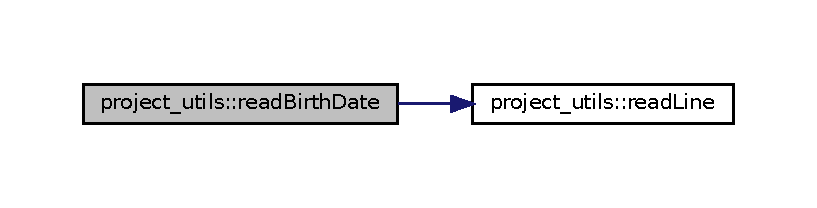
\includegraphics[width=350pt]{namespaceproject__utils_adab6593a2685f866191793214c7c60ce_cgraph}
\end{center}
\end{figure}
\mbox{\Hypertarget{namespaceproject__utils_a747fa96e998a1a6fb365d2512190098e}\label{namespaceproject__utils_a747fa96e998a1a6fb365d2512190098e}} 
\index{project\+\_\+utils@{project\+\_\+utils}!read\+Date@{read\+Date}}
\index{read\+Date@{read\+Date}!project\+\_\+utils@{project\+\_\+utils}}
\subsubsection{\texorpdfstring{read\+Date()}{readDate()}}
{\footnotesize\ttfamily \mbox{\hyperlink{classDate}{Date}} project\+\_\+utils\+::read\+Date (\begin{DoxyParamCaption}{ }\end{DoxyParamCaption})}



Read a date. 

Asks user to input a date in the format \char`\"{}dd-\/mm-\/yyyy H\+H\+:\+M\+M\char`\"{}.

\begin{DoxyReturn}{Returns}
\mbox{\hyperlink{classDate}{Date}} 
\end{DoxyReturn}
Here is the call graph for this function\+:
\nopagebreak
\begin{figure}[H]
\begin{center}
\leavevmode
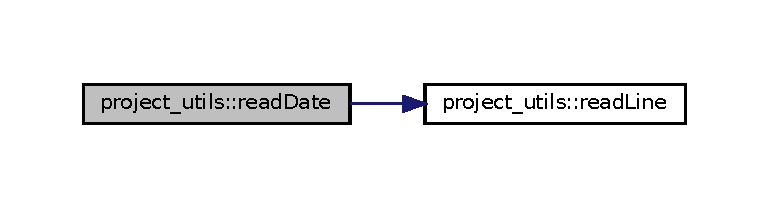
\includegraphics[width=350pt]{namespaceproject__utils_a747fa96e998a1a6fb365d2512190098e_cgraph}
\end{center}
\end{figure}
\mbox{\Hypertarget{namespaceproject__utils_aab1cf7fd8bfa2074ed3e6fb99fa973dc}\label{namespaceproject__utils_aab1cf7fd8bfa2074ed3e6fb99fa973dc}} 
\index{project\+\_\+utils@{project\+\_\+utils}!read\+Line@{read\+Line}}
\index{read\+Line@{read\+Line}!project\+\_\+utils@{project\+\_\+utils}}
\subsubsection{\texorpdfstring{read\+Line()}{readLine()}}
{\footnotesize\ttfamily bool project\+\_\+utils\+::read\+Line (\begin{DoxyParamCaption}\item[{string \&}]{s }\end{DoxyParamCaption})}



Function to read a string using getline(cin). 


\begin{DoxyParams}{Parameters}
{\em s} & \\
\hline
\end{DoxyParams}
\begin{DoxyReturn}{Returns}
true If cin reports E\+OF. 

false If cin doesn\textquotesingle{}t report E\+OF. 
\end{DoxyReturn}
\mbox{\Hypertarget{namespaceproject__utils_a72293f22700ff24cdf6663f45ca10c91}\label{namespaceproject__utils_a72293f22700ff24cdf6663f45ca10c91}} 
\index{project\+\_\+utils@{project\+\_\+utils}!read\+Var@{read\+Var}}
\index{read\+Var@{read\+Var}!project\+\_\+utils@{project\+\_\+utils}}
\subsubsection{\texorpdfstring{read\+Var()}{readVar()}}
{\footnotesize\ttfamily template$<$class T $>$ \\
bool project\+\_\+utils\+::read\+Var (\begin{DoxyParamCaption}\item[{T \&}]{var }\end{DoxyParamCaption})}



Template function to read any variable from cin. 


\begin{DoxyTemplParams}{Template Parameters}
{\em T} & \\
\hline
\end{DoxyTemplParams}

\begin{DoxyParams}{Parameters}
{\em var} & \\
\hline
\end{DoxyParams}
\begin{DoxyReturn}{Returns}
true If cin reports E\+OF. 

false IF cin doesn\textquotesingle{}t report E\+OF. 
\end{DoxyReturn}
\mbox{\Hypertarget{namespaceproject__utils_a8a3acf9a2b81c44b525870adb954dcff}\label{namespaceproject__utils_a8a3acf9a2b81c44b525870adb954dcff}} 
\index{project\+\_\+utils@{project\+\_\+utils}!split\+Arguments@{split\+Arguments}}
\index{split\+Arguments@{split\+Arguments}!project\+\_\+utils@{project\+\_\+utils}}
\subsubsection{\texorpdfstring{split\+Arguments()}{splitArguments()}}
{\footnotesize\ttfamily std\+::vector$<$std\+::string$>$ project\+\_\+utils\+::split\+Arguments (\begin{DoxyParamCaption}\item[{std\+::string \&}]{command }\end{DoxyParamCaption})}


\chapter{Class Documentation}
\hypertarget{classAlfaPendular}{}\section{Alfa\+Pendular Class Reference}
\label{classAlfaPendular}\index{Alfa\+Pendular@{Alfa\+Pendular}}


{\ttfamily \#include $<$Alfa\+Pendular.\+h$>$}



Inheritance diagram for Alfa\+Pendular\+:
\nopagebreak
\begin{figure}[H]
\begin{center}
\leavevmode
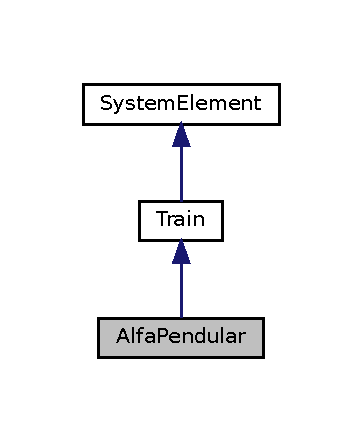
\includegraphics[width=174pt]{classAlfaPendular__inherit__graph}
\end{center}
\end{figure}


Collaboration diagram for Alfa\+Pendular\+:
\nopagebreak
\begin{figure}[H]
\begin{center}
\leavevmode
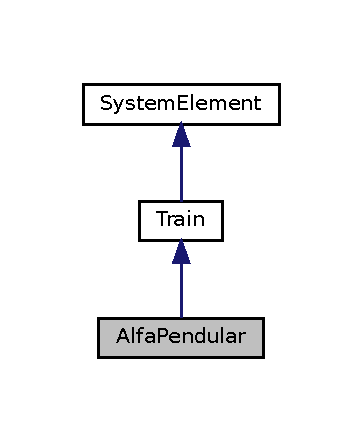
\includegraphics[width=174pt]{classAlfaPendular__coll__graph}
\end{center}
\end{figure}
\subsection*{Public Member Functions}
\begin{DoxyCompactItemize}
\item 
const char $\ast$ \mbox{\hyperlink{classAlfaPendular_a8bae5eb768c157fd2151dfb0d0134962}{get\+Type}} () const override
\item 
\mbox{\hyperlink{classAlfaPendular_ac194f781d3cb929f6ddcb5670dd7722d}{Alfa\+Pendular}} (\mbox{\hyperlink{project__utils_8h_a91ad9478d81a7aaf2593e8d9c3d06a14}{uint}} \mbox{\hyperlink{classTrain_a2954421b3beb871526ca169beca4c430}{max\+Seats}})
\item 
float \mbox{\hyperlink{classAlfaPendular_a12d09e5b65835ab7dcd3580ec8a41eee}{get\+Price\+Multiplyer}} () const override
\item 
void \mbox{\hyperlink{classAlfaPendular_aceb64b85c475612b8045d0108b448669}{print\+Row}} (std\+::ostream \&os) override
\end{DoxyCompactItemize}
\subsection*{Additional Inherited Members}


\subsection{Detailed Description}
Class representing an A\+Lfa Pendular train. Its a derivation of the \mbox{\hyperlink{classTrain}{Train}} class. 

\subsection{Constructor \& Destructor Documentation}
\mbox{\Hypertarget{classAlfaPendular_ac194f781d3cb929f6ddcb5670dd7722d}\label{classAlfaPendular_ac194f781d3cb929f6ddcb5670dd7722d}} 
\index{Alfa\+Pendular@{Alfa\+Pendular}!Alfa\+Pendular@{Alfa\+Pendular}}
\index{Alfa\+Pendular@{Alfa\+Pendular}!Alfa\+Pendular@{Alfa\+Pendular}}
\subsubsection{\texorpdfstring{Alfa\+Pendular()}{AlfaPendular()}}
{\footnotesize\ttfamily Alfa\+Pendular\+::\+Alfa\+Pendular (\begin{DoxyParamCaption}\item[{\mbox{\hyperlink{project__utils_8h_a91ad9478d81a7aaf2593e8d9c3d06a14}{uint}}}]{max\+Seats }\end{DoxyParamCaption})}

Construct a new \mbox{\hyperlink{classAlfaPendular}{Alfa\+Pendular}} object


\begin{DoxyParams}{Parameters}
{\em max\+Seats} & \\
\hline
\end{DoxyParams}


\subsection{Member Function Documentation}
\mbox{\Hypertarget{classAlfaPendular_a12d09e5b65835ab7dcd3580ec8a41eee}\label{classAlfaPendular_a12d09e5b65835ab7dcd3580ec8a41eee}} 
\index{Alfa\+Pendular@{Alfa\+Pendular}!get\+Price\+Multiplyer@{get\+Price\+Multiplyer}}
\index{get\+Price\+Multiplyer@{get\+Price\+Multiplyer}!Alfa\+Pendular@{Alfa\+Pendular}}
\subsubsection{\texorpdfstring{get\+Price\+Multiplyer()}{getPriceMultiplyer()}}
{\footnotesize\ttfamily float Alfa\+Pendular\+::get\+Price\+Multiplyer (\begin{DoxyParamCaption}{ }\end{DoxyParamCaption}) const\hspace{0.3cm}{\ttfamily [override]}, {\ttfamily [virtual]}}

\begin{DoxyReturn}{Returns}
2 
\end{DoxyReturn}


Implements \mbox{\hyperlink{classTrain_a2f8a45aaa96058a2675422d206221964}{Train}}.

\mbox{\Hypertarget{classAlfaPendular_a8bae5eb768c157fd2151dfb0d0134962}\label{classAlfaPendular_a8bae5eb768c157fd2151dfb0d0134962}} 
\index{Alfa\+Pendular@{Alfa\+Pendular}!get\+Type@{get\+Type}}
\index{get\+Type@{get\+Type}!Alfa\+Pendular@{Alfa\+Pendular}}
\subsubsection{\texorpdfstring{get\+Type()}{getType()}}
{\footnotesize\ttfamily const char $\ast$ Alfa\+Pendular\+::get\+Type (\begin{DoxyParamCaption}{ }\end{DoxyParamCaption}) const\hspace{0.3cm}{\ttfamily [override]}, {\ttfamily [virtual]}}

\begin{DoxyReturn}{Returns}
\char`\"{}\+A\+P\char`\"{} 
\end{DoxyReturn}


Implements \mbox{\hyperlink{classTrain_ad2bd424547b5be4e3fa8e491f1ce790d}{Train}}.

\mbox{\Hypertarget{classAlfaPendular_aceb64b85c475612b8045d0108b448669}\label{classAlfaPendular_aceb64b85c475612b8045d0108b448669}} 
\index{Alfa\+Pendular@{Alfa\+Pendular}!print\+Row@{print\+Row}}
\index{print\+Row@{print\+Row}!Alfa\+Pendular@{Alfa\+Pendular}}
\subsubsection{\texorpdfstring{print\+Row()}{printRow()}}
{\footnotesize\ttfamily void Alfa\+Pendular\+::print\+Row (\begin{DoxyParamCaption}\item[{std\+::ostream \&}]{os }\end{DoxyParamCaption})\hspace{0.3cm}{\ttfamily [override]}, {\ttfamily [virtual]}}

Print a formated row of the trains information. 

Reimplemented from \mbox{\hyperlink{classTrain_a3fd1c87c2152aa96cc6928f0aea37e21}{Train}}.



The documentation for this class was generated from the following files\+:\begin{DoxyCompactItemize}
\item 
system\+\_\+elements/\mbox{\hyperlink{AlfaPendular_8h}{Alfa\+Pendular.\+h}}\item 
system\+\_\+elements/\mbox{\hyperlink{AlfaPendular_8cpp}{Alfa\+Pendular.\+cpp}}\end{DoxyCompactItemize}

\hypertarget{classDate}{}\section{Date Class Reference}
\label{classDate}\index{Date@{Date}}


Class for representing dates in the program.  




{\ttfamily \#include $<$Date.\+h$>$}

\subsection*{Public Member Functions}
\begin{DoxyCompactItemize}
\item 
\mbox{\hyperlink{classDate_aa29ee0f04162437b91b758be0a4b75fc}{Date}} (int year, int month, int day, int hour=0, int minute=0)
\begin{DoxyCompactList}\small\item\em Construct a new \mbox{\hyperlink{classDate}{Date}} object. \end{DoxyCompactList}\item 
\mbox{\hyperlink{classDate_abaa8b0cf93eb1ad9206be4ff78ed2a3b}{Date}} (const std\+::string \&date\+String)
\begin{DoxyCompactList}\small\item\em Construct a new \mbox{\hyperlink{classDate}{Date}} object. \end{DoxyCompactList}\item 
bool \mbox{\hyperlink{classDate_a91ccc0361527f5f68785c5460d750a12}{operator==}} (\mbox{\hyperlink{classDate}{Date}} \&d)
\begin{DoxyCompactList}\small\item\em Check eqaulity between \mbox{\hyperlink{classDate}{Date}} objects. \end{DoxyCompactList}\item 
bool \mbox{\hyperlink{classDate_a51d1dadde23783adc9a2ae12d877803c}{operator$<$}} (\mbox{\hyperlink{classDate}{Date}} \&d)
\begin{DoxyCompactList}\small\item\em Check if \mbox{\hyperlink{classDate}{Date}} object happens before argument. \end{DoxyCompactList}\item 
bool \mbox{\hyperlink{classDate_a49b4e0ed6752c928164fd483720423da}{operator$<$=}} (\mbox{\hyperlink{classDate}{Date}} \&d)
\begin{DoxyCompactList}\small\item\em Check if \mbox{\hyperlink{classDate}{Date}} object happens before or at same time as argument. \end{DoxyCompactList}\item 
bool \mbox{\hyperlink{classDate_a0c2a1a6f890da1f9a360fab87e7109a3}{operator$>$}} (\mbox{\hyperlink{classDate}{Date}} \&d)
\begin{DoxyCompactList}\small\item\em Check if \mbox{\hyperlink{classDate}{Date}} object happens after argument. \end{DoxyCompactList}\item 
bool \mbox{\hyperlink{classDate_a3dd4c3c4818d69669927bec072ff85ce}{operator$>$=}} (\mbox{\hyperlink{classDate}{Date}} \&d)
\begin{DoxyCompactList}\small\item\em Check if \mbox{\hyperlink{classDate}{Date}} object happens after or at same time as argument. \end{DoxyCompactList}\item 
std\+::string \mbox{\hyperlink{classDate_a733c89177097f0d7f5cc2f68f5593856}{get\+Date\+String}} () const
\begin{DoxyCompactList}\small\item\em Get the \mbox{\hyperlink{classDate}{Date}} String. \end{DoxyCompactList}\item 
std\+::string \mbox{\hyperlink{classDate_a54b53336c8ba897fae4d2bbb0aa84a99}{get\+Date\+String\+Without\+Hours}} () const
\begin{DoxyCompactList}\small\item\em Get the \mbox{\hyperlink{classDate}{Date}} String Without Hours. \end{DoxyCompactList}\item 
int \mbox{\hyperlink{classDate_a8b0869f34c2b38d108ab83ee2e770e5d}{get\+Year}} () const
\begin{DoxyCompactList}\small\item\em Get the Year. \end{DoxyCompactList}\item 
int \mbox{\hyperlink{classDate_a332f6e3a2f6a40d73742b6dab7be0f64}{get\+Month}} () const
\begin{DoxyCompactList}\small\item\em Get the Month. \end{DoxyCompactList}\item 
int \mbox{\hyperlink{classDate_a0f253815240e70f4c39cb93cc68bd3f4}{get\+Day}} () const
\begin{DoxyCompactList}\small\item\em Get the Day. \end{DoxyCompactList}\item 
int \mbox{\hyperlink{classDate_ab8ea9e1aafa6cb95be7b82cda0c53cfe}{get\+Hour}} () const
\begin{DoxyCompactList}\small\item\em Get the Hour. \end{DoxyCompactList}\item 
int \mbox{\hyperlink{classDate_a55251df891f43b9f19419cd79ce69876}{get\+Minutes}} () const
\begin{DoxyCompactList}\small\item\em Get the Minutes. \end{DoxyCompactList}\item 
long int \mbox{\hyperlink{classDate_af047ef9ca2cf7843b921f36e9883f0a7}{get\+Time\+Stamp}} ()
\begin{DoxyCompactList}\small\item\em Get the Time Stamp object. \end{DoxyCompactList}\end{DoxyCompactItemize}
\subsection*{Friends}
\begin{DoxyCompactItemize}
\item 
std\+::ostream \& \mbox{\hyperlink{classDate_a2f114c7aa1398dac0f21b888bcb40f3e}{operator$<$$<$}} (std\+::ostream \&o, \mbox{\hyperlink{classDate}{Date}} \&d)
\begin{DoxyCompactList}\small\item\em ouput \mbox{\hyperlink{classDate}{Date}} object into an output stream \end{DoxyCompactList}\end{DoxyCompactItemize}


\subsection{Detailed Description}
Class for representing dates in the program. 

Works as an abstraction of C++\textquotesingle{}s ctime library. 

\subsection{Constructor \& Destructor Documentation}
\mbox{\Hypertarget{classDate_aa29ee0f04162437b91b758be0a4b75fc}\label{classDate_aa29ee0f04162437b91b758be0a4b75fc}} 
\index{Date@{Date}!Date@{Date}}
\index{Date@{Date}!Date@{Date}}
\subsubsection{\texorpdfstring{Date()}{Date()}\hspace{0.1cm}{\footnotesize\ttfamily [1/2]}}
{\footnotesize\ttfamily Date\+::\+Date (\begin{DoxyParamCaption}\item[{int}]{year,  }\item[{int}]{month,  }\item[{int}]{day,  }\item[{int}]{hour = {\ttfamily 0},  }\item[{int}]{minute = {\ttfamily 0} }\end{DoxyParamCaption})}



Construct a new \mbox{\hyperlink{classDate}{Date}} object. 

Constructs \mbox{\hyperlink{classDate}{Date}} object and calls validate(). If validation fails, throws Invalid\+Date\+Exception.


\begin{DoxyParams}{Parameters}
{\em year} & \mbox{\hyperlink{classDate}{Date}}\textquotesingle{}s year \\
\hline
{\em month} & \mbox{\hyperlink{classDate}{Date}}\textquotesingle{}s month \\
\hline
{\em day} & \mbox{\hyperlink{classDate}{Date}}\textquotesingle{}s day in month \\
\hline
{\em hour} & \mbox{\hyperlink{classDate}{Date}}\textquotesingle{}s hour of day (24h format) \\
\hline
{\em minute} & \mbox{\hyperlink{classDate}{Date}}\textquotesingle{}s minutes \\
\hline
\end{DoxyParams}
\mbox{\Hypertarget{classDate_abaa8b0cf93eb1ad9206be4ff78ed2a3b}\label{classDate_abaa8b0cf93eb1ad9206be4ff78ed2a3b}} 
\index{Date@{Date}!Date@{Date}}
\index{Date@{Date}!Date@{Date}}
\subsubsection{\texorpdfstring{Date()}{Date()}\hspace{0.1cm}{\footnotesize\ttfamily [2/2]}}
{\footnotesize\ttfamily Date\+::\+Date (\begin{DoxyParamCaption}\item[{const std\+::string \&}]{date\+String }\end{DoxyParamCaption})}



Construct a new \mbox{\hyperlink{classDate}{Date}} object. 

Constructs \mbox{\hyperlink{classDate}{Date}} object and calls validate(). If validation fails, throws Invalid\+Date\+Exception.


\begin{DoxyParams}{Parameters}
{\em date\+String} & \mbox{\hyperlink{classDate}{Date}} in form of a string in format \char`\"{}dd-\/mm-\/yyyy H\+H\+:\+M\+M\char`\"{}. Day, month, year, hour and minutes must be two digits (\textquotesingle{}02\textquotesingle{}, \textquotesingle{}08\textquotesingle{}, \textquotesingle{}12\textquotesingle{}) \\
\hline
\end{DoxyParams}


\subsection{Member Function Documentation}
\mbox{\Hypertarget{classDate_a733c89177097f0d7f5cc2f68f5593856}\label{classDate_a733c89177097f0d7f5cc2f68f5593856}} 
\index{Date@{Date}!get\+Date\+String@{get\+Date\+String}}
\index{get\+Date\+String@{get\+Date\+String}!Date@{Date}}
\subsubsection{\texorpdfstring{get\+Date\+String()}{getDateString()}}
{\footnotesize\ttfamily std\+::string Date\+::get\+Date\+String (\begin{DoxyParamCaption}{ }\end{DoxyParamCaption}) const}



Get the \mbox{\hyperlink{classDate}{Date}} String. 

\begin{DoxyReturn}{Returns}
std\+::string a string in the format\+: \char`\"{}dd-\/mm-\/yyyy H\+H\+:\+M\+M\char`\"{} 
\end{DoxyReturn}
\mbox{\Hypertarget{classDate_a54b53336c8ba897fae4d2bbb0aa84a99}\label{classDate_a54b53336c8ba897fae4d2bbb0aa84a99}} 
\index{Date@{Date}!get\+Date\+String\+Without\+Hours@{get\+Date\+String\+Without\+Hours}}
\index{get\+Date\+String\+Without\+Hours@{get\+Date\+String\+Without\+Hours}!Date@{Date}}
\subsubsection{\texorpdfstring{get\+Date\+String\+Without\+Hours()}{getDateStringWithoutHours()}}
{\footnotesize\ttfamily std\+::string Date\+::get\+Date\+String\+Without\+Hours (\begin{DoxyParamCaption}{ }\end{DoxyParamCaption}) const}



Get the \mbox{\hyperlink{classDate}{Date}} String Without Hours. 

\begin{DoxyReturn}{Returns}
std\+::string a string in the format\+: \char`\"{}dd-\/mm-\/yyyy\char`\"{} 
\end{DoxyReturn}
\mbox{\Hypertarget{classDate_a0f253815240e70f4c39cb93cc68bd3f4}\label{classDate_a0f253815240e70f4c39cb93cc68bd3f4}} 
\index{Date@{Date}!get\+Day@{get\+Day}}
\index{get\+Day@{get\+Day}!Date@{Date}}
\subsubsection{\texorpdfstring{get\+Day()}{getDay()}}
{\footnotesize\ttfamily int Date\+::get\+Day (\begin{DoxyParamCaption}{ }\end{DoxyParamCaption}) const}



Get the Day. 

\begin{DoxyReturn}{Returns}
int 
\end{DoxyReturn}
\mbox{\Hypertarget{classDate_ab8ea9e1aafa6cb95be7b82cda0c53cfe}\label{classDate_ab8ea9e1aafa6cb95be7b82cda0c53cfe}} 
\index{Date@{Date}!get\+Hour@{get\+Hour}}
\index{get\+Hour@{get\+Hour}!Date@{Date}}
\subsubsection{\texorpdfstring{get\+Hour()}{getHour()}}
{\footnotesize\ttfamily int Date\+::get\+Hour (\begin{DoxyParamCaption}{ }\end{DoxyParamCaption}) const}



Get the Hour. 

\begin{DoxyReturn}{Returns}
int 
\end{DoxyReturn}
\mbox{\Hypertarget{classDate_a55251df891f43b9f19419cd79ce69876}\label{classDate_a55251df891f43b9f19419cd79ce69876}} 
\index{Date@{Date}!get\+Minutes@{get\+Minutes}}
\index{get\+Minutes@{get\+Minutes}!Date@{Date}}
\subsubsection{\texorpdfstring{get\+Minutes()}{getMinutes()}}
{\footnotesize\ttfamily int Date\+::get\+Minutes (\begin{DoxyParamCaption}{ }\end{DoxyParamCaption}) const}



Get the Minutes. 

\begin{DoxyReturn}{Returns}
int 
\end{DoxyReturn}
\mbox{\Hypertarget{classDate_a332f6e3a2f6a40d73742b6dab7be0f64}\label{classDate_a332f6e3a2f6a40d73742b6dab7be0f64}} 
\index{Date@{Date}!get\+Month@{get\+Month}}
\index{get\+Month@{get\+Month}!Date@{Date}}
\subsubsection{\texorpdfstring{get\+Month()}{getMonth()}}
{\footnotesize\ttfamily int Date\+::get\+Month (\begin{DoxyParamCaption}{ }\end{DoxyParamCaption}) const}



Get the Month. 

\begin{DoxyReturn}{Returns}
int 
\end{DoxyReturn}
\mbox{\Hypertarget{classDate_af047ef9ca2cf7843b921f36e9883f0a7}\label{classDate_af047ef9ca2cf7843b921f36e9883f0a7}} 
\index{Date@{Date}!get\+Time\+Stamp@{get\+Time\+Stamp}}
\index{get\+Time\+Stamp@{get\+Time\+Stamp}!Date@{Date}}
\subsubsection{\texorpdfstring{get\+Time\+Stamp()}{getTimeStamp()}}
{\footnotesize\ttfamily long int Date\+::get\+Time\+Stamp (\begin{DoxyParamCaption}{ }\end{DoxyParamCaption})}



Get the Time Stamp object. 

\begin{DoxyReturn}{Returns}
long Seconds since epoch at January 1st 1970 00\+:00 
\end{DoxyReturn}
\mbox{\Hypertarget{classDate_a8b0869f34c2b38d108ab83ee2e770e5d}\label{classDate_a8b0869f34c2b38d108ab83ee2e770e5d}} 
\index{Date@{Date}!get\+Year@{get\+Year}}
\index{get\+Year@{get\+Year}!Date@{Date}}
\subsubsection{\texorpdfstring{get\+Year()}{getYear()}}
{\footnotesize\ttfamily int Date\+::get\+Year (\begin{DoxyParamCaption}{ }\end{DoxyParamCaption}) const}



Get the Year. 

\begin{DoxyReturn}{Returns}
int 
\end{DoxyReturn}
\mbox{\Hypertarget{classDate_a51d1dadde23783adc9a2ae12d877803c}\label{classDate_a51d1dadde23783adc9a2ae12d877803c}} 
\index{Date@{Date}!operator$<$@{operator$<$}}
\index{operator$<$@{operator$<$}!Date@{Date}}
\subsubsection{\texorpdfstring{operator$<$()}{operator<()}}
{\footnotesize\ttfamily bool Date\+::operator$<$ (\begin{DoxyParamCaption}\item[{\mbox{\hyperlink{classDate}{Date}} \&}]{d }\end{DoxyParamCaption})}



Check if \mbox{\hyperlink{classDate}{Date}} object happens before argument. 


\begin{DoxyParams}{Parameters}
{\em d} & \mbox{\hyperlink{classDate}{Date}} object to compare \\
\hline
\end{DoxyParams}
\begin{DoxyReturn}{Returns}
true if object happens before argument 

false if otherwise 
\end{DoxyReturn}
\mbox{\Hypertarget{classDate_a49b4e0ed6752c928164fd483720423da}\label{classDate_a49b4e0ed6752c928164fd483720423da}} 
\index{Date@{Date}!operator$<$=@{operator$<$=}}
\index{operator$<$=@{operator$<$=}!Date@{Date}}
\subsubsection{\texorpdfstring{operator$<$=()}{operator<=()}}
{\footnotesize\ttfamily bool Date\+::operator$<$= (\begin{DoxyParamCaption}\item[{\mbox{\hyperlink{classDate}{Date}} \&}]{d }\end{DoxyParamCaption})}



Check if \mbox{\hyperlink{classDate}{Date}} object happens before or at same time as argument. 


\begin{DoxyParams}{Parameters}
{\em d} & \mbox{\hyperlink{classDate}{Date}} object to compare with self \\
\hline
\end{DoxyParams}
\begin{DoxyReturn}{Returns}
true if object happens before or at same time of argument 

false if otherwise 
\end{DoxyReturn}
\mbox{\Hypertarget{classDate_a91ccc0361527f5f68785c5460d750a12}\label{classDate_a91ccc0361527f5f68785c5460d750a12}} 
\index{Date@{Date}!operator==@{operator==}}
\index{operator==@{operator==}!Date@{Date}}
\subsubsection{\texorpdfstring{operator==()}{operator==()}}
{\footnotesize\ttfamily bool Date\+::operator== (\begin{DoxyParamCaption}\item[{\mbox{\hyperlink{classDate}{Date}} \&}]{d }\end{DoxyParamCaption})}



Check eqaulity between \mbox{\hyperlink{classDate}{Date}} objects. 


\begin{DoxyParams}{Parameters}
{\em d} & \mbox{\hyperlink{classDate}{Date}} object to compare with self \\
\hline
\end{DoxyParams}
\begin{DoxyReturn}{Returns}
true if equal 

false if not equal 
\end{DoxyReturn}
\mbox{\Hypertarget{classDate_a0c2a1a6f890da1f9a360fab87e7109a3}\label{classDate_a0c2a1a6f890da1f9a360fab87e7109a3}} 
\index{Date@{Date}!operator$>$@{operator$>$}}
\index{operator$>$@{operator$>$}!Date@{Date}}
\subsubsection{\texorpdfstring{operator$>$()}{operator>()}}
{\footnotesize\ttfamily bool Date\+::operator$>$ (\begin{DoxyParamCaption}\item[{\mbox{\hyperlink{classDate}{Date}} \&}]{d }\end{DoxyParamCaption})}



Check if \mbox{\hyperlink{classDate}{Date}} object happens after argument. 


\begin{DoxyParams}{Parameters}
{\em d} & \mbox{\hyperlink{classDate}{Date}} object to compare with self \\
\hline
\end{DoxyParams}
\begin{DoxyReturn}{Returns}
true if object happens after argument 

false if otherwise 
\end{DoxyReturn}
\mbox{\Hypertarget{classDate_a3dd4c3c4818d69669927bec072ff85ce}\label{classDate_a3dd4c3c4818d69669927bec072ff85ce}} 
\index{Date@{Date}!operator$>$=@{operator$>$=}}
\index{operator$>$=@{operator$>$=}!Date@{Date}}
\subsubsection{\texorpdfstring{operator$>$=()}{operator>=()}}
{\footnotesize\ttfamily bool Date\+::operator$>$= (\begin{DoxyParamCaption}\item[{\mbox{\hyperlink{classDate}{Date}} \&}]{d }\end{DoxyParamCaption})}



Check if \mbox{\hyperlink{classDate}{Date}} object happens after or at same time as argument. 


\begin{DoxyParams}{Parameters}
{\em d} & \mbox{\hyperlink{classDate}{Date}} object to compare with self \\
\hline
\end{DoxyParams}
\begin{DoxyReturn}{Returns}
true if object happens after or at same time of argument 

false if otherwise 
\end{DoxyReturn}


\subsection{Friends And Related Function Documentation}
\mbox{\Hypertarget{classDate_a2f114c7aa1398dac0f21b888bcb40f3e}\label{classDate_a2f114c7aa1398dac0f21b888bcb40f3e}} 
\index{Date@{Date}!operator$<$$<$@{operator$<$$<$}}
\index{operator$<$$<$@{operator$<$$<$}!Date@{Date}}
\subsubsection{\texorpdfstring{operator$<$$<$}{operator<<}}
{\footnotesize\ttfamily std\+::ostream\& operator$<$$<$ (\begin{DoxyParamCaption}\item[{std\+::ostream \&}]{o,  }\item[{\mbox{\hyperlink{classDate}{Date}} \&}]{d }\end{DoxyParamCaption})\hspace{0.3cm}{\ttfamily [friend]}}



ouput \mbox{\hyperlink{classDate}{Date}} object into an output stream 

Passes a string of the date, to the output stream, in the following format\+: \char`\"{}dd-\/mm-\/yyyy H\+H\+:\+M\+M\char`\"{}


\begin{DoxyParams}{Parameters}
{\em o} & ouput stream \\
\hline
{\em d} & date object \\
\hline
\end{DoxyParams}
\begin{DoxyReturn}{Returns}
std\+::ostream\& reference to the output stream passed as argument 
\end{DoxyReturn}


The documentation for this class was generated from the following files\+:\begin{DoxyCompactItemize}
\item 
Date.\+h\item 
Date.\+cpp\end{DoxyCompactItemize}

\hypertarget{classEngineer}{}\section{Engineer Class Reference}
\label{classEngineer}\index{Engineer@{Engineer}}


{\ttfamily \#include $<$Engineer.\+h$>$}



Inheritance diagram for Engineer\+:
\nopagebreak
\begin{figure}[H]
\begin{center}
\leavevmode
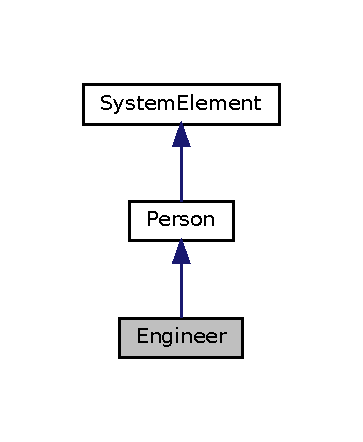
\includegraphics[width=174pt]{classEngineer__inherit__graph}
\end{center}
\end{figure}


Collaboration diagram for Engineer\+:
\nopagebreak
\begin{figure}[H]
\begin{center}
\leavevmode
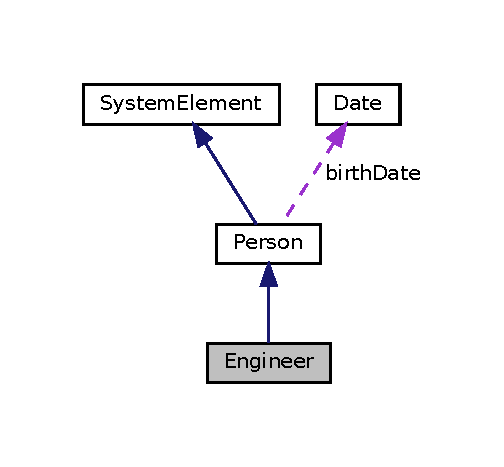
\includegraphics[width=242pt]{classEngineer__coll__graph}
\end{center}
\end{figure}
\subsection*{Classes}
\begin{DoxyCompactItemize}
\item 
struct \mbox{\hyperlink{structEngineer_1_1EngineerHashUtils}{Engineer\+Hash\+Utils}}
\end{DoxyCompactItemize}
\subsection*{Public Member Functions}
\begin{DoxyCompactItemize}
\item 
\mbox{\hyperlink{classEngineer_a608c643d1826e12d503c213679803a60}{Engineer}} (std\+::string \mbox{\hyperlink{classPerson_a7594663aadc0de77616506df8a2f4128}{name}}, \mbox{\hyperlink{classDate}{Date}} \mbox{\hyperlink{classPerson_a7a764b56b815321eeb8412c1dcc4cabf}{birth\+Date}})
\item 
\mbox{\hyperlink{project__utils_8h_a8f3a969054ad2200720b96e7e23dd4e1}{id\+\_\+t}} \mbox{\hyperlink{classEngineer_aa2a341b66e189ef19ab7dfa364cd2c20}{get\+ID}} () const
\item 
void \mbox{\hyperlink{classEngineer_ad413cf55ffbef71b3d5d58aa522da8cf}{set\+ID}} (\mbox{\hyperlink{project__utils_8h_a8f3a969054ad2200720b96e7e23dd4e1}{id\+\_\+t}} id)
\item 
void \mbox{\hyperlink{classEngineer_a399ceec45f4608f743070893ac573dcc}{add\+Trip}} (\mbox{\hyperlink{classTrip}{Trip}} $\ast$trip)
\item 
std\+::set$<$ \mbox{\hyperlink{classTrip}{Trip}} $\ast$ $>$ \mbox{\hyperlink{classEngineer_af2dd8a34a1f90956e9c31043638518cf}{get\+Trips}} ()
\item 
void \mbox{\hyperlink{classEngineer_a75fdfc733d86cb8dc2ff243994716da1}{print\+Row}} (std\+::ostream \&os)
\end{DoxyCompactItemize}
\subsection*{Additional Inherited Members}


\subsection{Detailed Description}
Class representing an engineer(train driver). Extends class \mbox{\hyperlink{classPerson}{Person}}. 

\subsection{Constructor \& Destructor Documentation}
\mbox{\Hypertarget{classEngineer_a608c643d1826e12d503c213679803a60}\label{classEngineer_a608c643d1826e12d503c213679803a60}} 
\index{Engineer@{Engineer}!Engineer@{Engineer}}
\index{Engineer@{Engineer}!Engineer@{Engineer}}
\subsubsection{\texorpdfstring{Engineer()}{Engineer()}}
{\footnotesize\ttfamily Engineer\+::\+Engineer (\begin{DoxyParamCaption}\item[{std\+::string}]{name,  }\item[{\mbox{\hyperlink{classDate}{Date}}}]{birth\+Date }\end{DoxyParamCaption})}

Construct a new \mbox{\hyperlink{classEngineer}{Engineer}} object.


\begin{DoxyParams}{Parameters}
{\em name} & \\
\hline
{\em birth\+Date} & \\
\hline
\end{DoxyParams}


\subsection{Member Function Documentation}
\mbox{\Hypertarget{classEngineer_a399ceec45f4608f743070893ac573dcc}\label{classEngineer_a399ceec45f4608f743070893ac573dcc}} 
\index{Engineer@{Engineer}!add\+Trip@{add\+Trip}}
\index{add\+Trip@{add\+Trip}!Engineer@{Engineer}}
\subsubsection{\texorpdfstring{add\+Trip()}{addTrip()}}
{\footnotesize\ttfamily void Engineer\+::add\+Trip (\begin{DoxyParamCaption}\item[{\mbox{\hyperlink{classTrip}{Trip}} $\ast$}]{trip }\end{DoxyParamCaption})}

Add a trip to the engineer\textquotesingle{}s trip history.


\begin{DoxyParams}{Parameters}
{\em trip} & \\
\hline
\end{DoxyParams}
\mbox{\Hypertarget{classEngineer_aa2a341b66e189ef19ab7dfa364cd2c20}\label{classEngineer_aa2a341b66e189ef19ab7dfa364cd2c20}} 
\index{Engineer@{Engineer}!get\+ID@{get\+ID}}
\index{get\+ID@{get\+ID}!Engineer@{Engineer}}
\subsubsection{\texorpdfstring{get\+I\+D()}{getID()}}
{\footnotesize\ttfamily \mbox{\hyperlink{project__utils_8h_a8f3a969054ad2200720b96e7e23dd4e1}{id\+\_\+t}} Engineer\+::get\+ID (\begin{DoxyParamCaption}{ }\end{DoxyParamCaption}) const}

Get the engineer ID.

\begin{DoxyReturn}{Returns}

\end{DoxyReturn}
\mbox{\Hypertarget{classEngineer_af2dd8a34a1f90956e9c31043638518cf}\label{classEngineer_af2dd8a34a1f90956e9c31043638518cf}} 
\index{Engineer@{Engineer}!get\+Trips@{get\+Trips}}
\index{get\+Trips@{get\+Trips}!Engineer@{Engineer}}
\subsubsection{\texorpdfstring{get\+Trips()}{getTrips()}}
{\footnotesize\ttfamily std\+::set$<$ \mbox{\hyperlink{classTrip}{Trip}} $\ast$ $>$ Engineer\+::get\+Trips (\begin{DoxyParamCaption}{ }\end{DoxyParamCaption})}

Get the vector of trips made by the engineer.

\begin{DoxyReturn}{Returns}

\end{DoxyReturn}
\mbox{\Hypertarget{classEngineer_a75fdfc733d86cb8dc2ff243994716da1}\label{classEngineer_a75fdfc733d86cb8dc2ff243994716da1}} 
\index{Engineer@{Engineer}!print\+Row@{print\+Row}}
\index{print\+Row@{print\+Row}!Engineer@{Engineer}}
\subsubsection{\texorpdfstring{print\+Row()}{printRow()}}
{\footnotesize\ttfamily void Engineer\+::print\+Row (\begin{DoxyParamCaption}\item[{std\+::ostream \&}]{os }\end{DoxyParamCaption})}

Print the engineer information in a formatted row.


\begin{DoxyParams}{Parameters}
{\em os} & \\
\hline
\end{DoxyParams}
Here is the call graph for this function\+:
\nopagebreak
\begin{figure}[H]
\begin{center}
\leavevmode
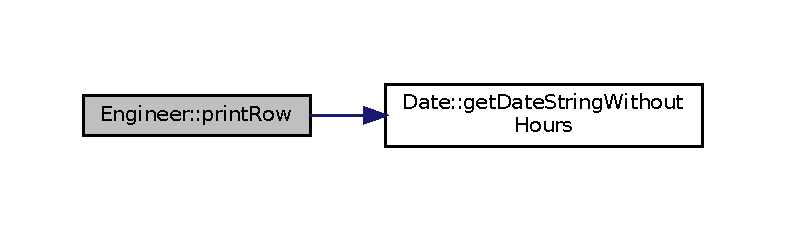
\includegraphics[width=350pt]{classEngineer_a75fdfc733d86cb8dc2ff243994716da1_cgraph}
\end{center}
\end{figure}
\mbox{\Hypertarget{classEngineer_ad413cf55ffbef71b3d5d58aa522da8cf}\label{classEngineer_ad413cf55ffbef71b3d5d58aa522da8cf}} 
\index{Engineer@{Engineer}!set\+ID@{set\+ID}}
\index{set\+ID@{set\+ID}!Engineer@{Engineer}}
\subsubsection{\texorpdfstring{set\+I\+D()}{setID()}}
{\footnotesize\ttfamily void Engineer\+::set\+ID (\begin{DoxyParamCaption}\item[{\mbox{\hyperlink{project__utils_8h_a8f3a969054ad2200720b96e7e23dd4e1}{id\+\_\+t}}}]{id }\end{DoxyParamCaption})}

Set the engineer ID.


\begin{DoxyParams}{Parameters}
{\em id} & \\
\hline
\end{DoxyParams}


The documentation for this class was generated from the following files\+:\begin{DoxyCompactItemize}
\item 
system\+\_\+elements/\mbox{\hyperlink{Engineer_8h}{Engineer.\+h}}\item 
system\+\_\+elements/\mbox{\hyperlink{Engineer_8cpp}{Engineer.\+cpp}}\end{DoxyCompactItemize}

\hypertarget{structEngineer_1_1EngineerHashUtils}{}\section{Engineer\+:\+:Engineer\+Hash\+Utils Struct Reference}
\label{structEngineer_1_1EngineerHashUtils}\index{Engineer\+::\+Engineer\+Hash\+Utils@{Engineer\+::\+Engineer\+Hash\+Utils}}


{\ttfamily \#include $<$Engineer.\+h$>$}

\subsection*{Public Member Functions}
\begin{DoxyCompactItemize}
\item 
int \mbox{\hyperlink{structEngineer_1_1EngineerHashUtils_aa6e83d6d97278db4aad2f07a2cd42cb4}{operator()}} (\mbox{\hyperlink{classEngineer}{Engineer}} $\ast$e) const
\item 
bool \mbox{\hyperlink{structEngineer_1_1EngineerHashUtils_a4af5919a2a9ff2efd3ae3ec9171919d0}{operator()}} (const \mbox{\hyperlink{classEngineer}{Engineer}} $\ast$e1, const \mbox{\hyperlink{classEngineer}{Engineer}} $\ast$e2) const
\end{DoxyCompactItemize}


\subsection{Detailed Description}
Struct with function operator overrides to be provided to \mbox{\hyperlink{classEngineer}{Engineer}} hash map. 

\subsection{Member Function Documentation}
\mbox{\Hypertarget{structEngineer_1_1EngineerHashUtils_aa6e83d6d97278db4aad2f07a2cd42cb4}\label{structEngineer_1_1EngineerHashUtils_aa6e83d6d97278db4aad2f07a2cd42cb4}} 
\index{Engineer\+::\+Engineer\+Hash\+Utils@{Engineer\+::\+Engineer\+Hash\+Utils}!operator()@{operator()}}
\index{operator()@{operator()}!Engineer\+::\+Engineer\+Hash\+Utils@{Engineer\+::\+Engineer\+Hash\+Utils}}
\subsubsection{\texorpdfstring{operator()()}{operator()()}\hspace{0.1cm}{\footnotesize\ttfamily [1/2]}}
{\footnotesize\ttfamily int Engineer\+::\+Engineer\+Hash\+Utils\+::operator() (\begin{DoxyParamCaption}\item[{\mbox{\hyperlink{classEngineer}{Engineer}} $\ast$}]{e }\end{DoxyParamCaption}) const\hspace{0.3cm}{\ttfamily [inline]}}

\mbox{\hyperlink{classEngineer}{Engineer}} hash function.


\begin{DoxyParams}{Parameters}
{\em e} & \\
\hline
\end{DoxyParams}
\begin{DoxyReturn}{Returns}
Index 
\end{DoxyReturn}
Here is the call graph for this function\+:
\nopagebreak
\begin{figure}[H]
\begin{center}
\leavevmode
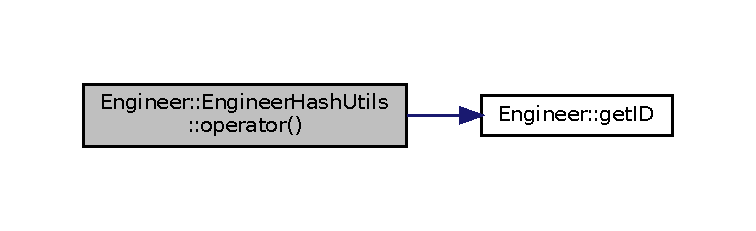
\includegraphics[width=350pt]{structEngineer_1_1EngineerHashUtils_aa6e83d6d97278db4aad2f07a2cd42cb4_cgraph}
\end{center}
\end{figure}
\mbox{\Hypertarget{structEngineer_1_1EngineerHashUtils_a4af5919a2a9ff2efd3ae3ec9171919d0}\label{structEngineer_1_1EngineerHashUtils_a4af5919a2a9ff2efd3ae3ec9171919d0}} 
\index{Engineer\+::\+Engineer\+Hash\+Utils@{Engineer\+::\+Engineer\+Hash\+Utils}!operator()@{operator()}}
\index{operator()@{operator()}!Engineer\+::\+Engineer\+Hash\+Utils@{Engineer\+::\+Engineer\+Hash\+Utils}}
\subsubsection{\texorpdfstring{operator()()}{operator()()}\hspace{0.1cm}{\footnotesize\ttfamily [2/2]}}
{\footnotesize\ttfamily bool Engineer\+::\+Engineer\+Hash\+Utils\+::operator() (\begin{DoxyParamCaption}\item[{const \mbox{\hyperlink{classEngineer}{Engineer}} $\ast$}]{e1,  }\item[{const \mbox{\hyperlink{classEngineer}{Engineer}} $\ast$}]{e2 }\end{DoxyParamCaption}) const\hspace{0.3cm}{\ttfamily [inline]}}

\mbox{\hyperlink{classEngineer}{Engineer}} equivalence function.


\begin{DoxyParams}{Parameters}
{\em e1} & \\
\hline
{\em e2} & \\
\hline
\end{DoxyParams}
\begin{DoxyReturn}{Returns}

\end{DoxyReturn}
Here is the call graph for this function\+:
\nopagebreak
\begin{figure}[H]
\begin{center}
\leavevmode
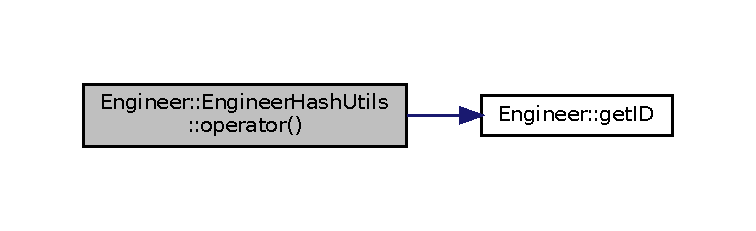
\includegraphics[width=350pt]{structEngineer_1_1EngineerHashUtils_a4af5919a2a9ff2efd3ae3ec9171919d0_cgraph}
\end{center}
\end{figure}


The documentation for this struct was generated from the following file\+:\begin{DoxyCompactItemize}
\item 
system\+\_\+elements/\mbox{\hyperlink{Engineer_8h}{Engineer.\+h}}\end{DoxyCompactItemize}

\hypertarget{classIdenticalDestinationException}{}\section{Identical\+Destination\+Exception Class Reference}
\label{classIdenticalDestinationException}\index{Identical\+Destination\+Exception@{Identical\+Destination\+Exception}}


Exception reporting when a trip has destination identical to source.  




{\ttfamily \#include $<$Identical\+Destination\+Exception.\+h$>$}



Inheritance diagram for Identical\+Destination\+Exception\+:
\nopagebreak
\begin{figure}[H]
\begin{center}
\leavevmode
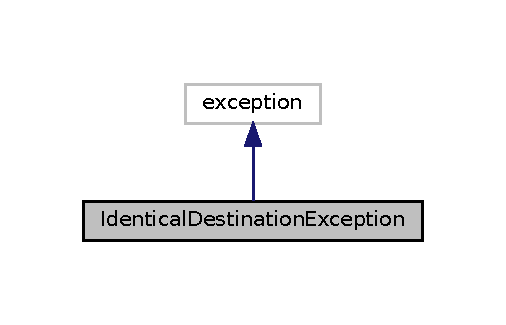
\includegraphics[width=243pt]{classIdenticalDestinationException__inherit__graph}
\end{center}
\end{figure}


Collaboration diagram for Identical\+Destination\+Exception\+:
\nopagebreak
\begin{figure}[H]
\begin{center}
\leavevmode
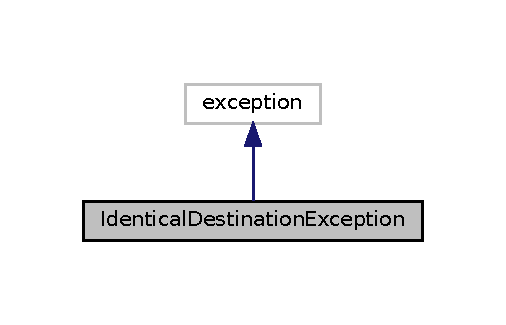
\includegraphics[width=243pt]{classIdenticalDestinationException__coll__graph}
\end{center}
\end{figure}
\subsection*{Public Member Functions}
\begin{DoxyCompactItemize}
\item 
const char $\ast$ \mbox{\hyperlink{classIdenticalDestinationException_ae07860f180405086788815185b3525b1}{what}} ()
\end{DoxyCompactItemize}


\subsection{Detailed Description}
Exception reporting when a trip has destination identical to source. 

\subsection{Member Function Documentation}
\mbox{\Hypertarget{classIdenticalDestinationException_ae07860f180405086788815185b3525b1}\label{classIdenticalDestinationException_ae07860f180405086788815185b3525b1}} 
\index{Identical\+Destination\+Exception@{Identical\+Destination\+Exception}!what@{what}}
\index{what@{what}!Identical\+Destination\+Exception@{Identical\+Destination\+Exception}}
\subsubsection{\texorpdfstring{what()}{what()}}
{\footnotesize\ttfamily const char $\ast$ Identical\+Destination\+Exception\+::what (\begin{DoxyParamCaption}{ }\end{DoxyParamCaption})}



The documentation for this class was generated from the following files\+:\begin{DoxyCompactItemize}
\item 
exceptions/\mbox{\hyperlink{IdenticalDestinationException_8h}{Identical\+Destination\+Exception.\+h}}\item 
exceptions/\mbox{\hyperlink{IdenticalDestinationException_8cpp}{Identical\+Destination\+Exception.\+cpp}}\end{DoxyCompactItemize}

\hypertarget{classInterCidades}{}\section{Inter\+Cidades Class Reference}
\label{classInterCidades}\index{Inter\+Cidades@{Inter\+Cidades}}


{\ttfamily \#include $<$Inter\+Cidades.\+h$>$}



Inheritance diagram for Inter\+Cidades\+:
\nopagebreak
\begin{figure}[H]
\begin{center}
\leavevmode
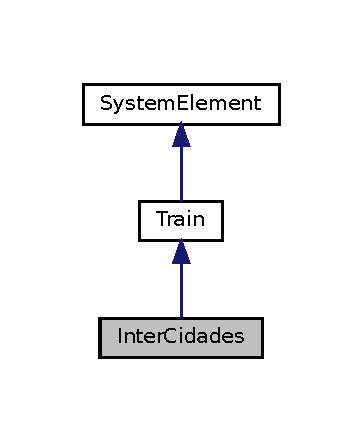
\includegraphics[width=174pt]{classInterCidades__inherit__graph}
\end{center}
\end{figure}


Collaboration diagram for Inter\+Cidades\+:
\nopagebreak
\begin{figure}[H]
\begin{center}
\leavevmode
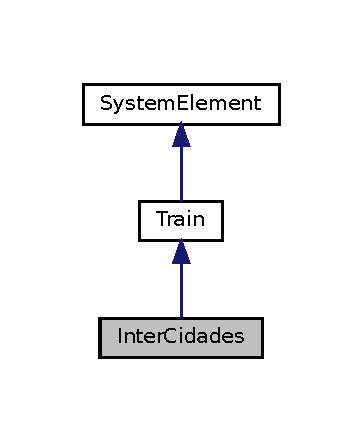
\includegraphics[width=174pt]{classInterCidades__coll__graph}
\end{center}
\end{figure}
\subsection*{Public Member Functions}
\begin{DoxyCompactItemize}
\item 
\mbox{\hyperlink{classInterCidades_a461d109be503396d4c66a5016438bb26}{Inter\+Cidades}} (\mbox{\hyperlink{project__utils_8h_a91ad9478d81a7aaf2593e8d9c3d06a14}{uint}} \mbox{\hyperlink{classTrain_a2954421b3beb871526ca169beca4c430}{max\+Seats}})
\item 
const char $\ast$ \mbox{\hyperlink{classInterCidades_a19eb37a1538d16247a7ba44e4a3c367b}{get\+Type}} () const override
\item 
float \mbox{\hyperlink{classInterCidades_ae48f10e5086edea5b9797ae12ab0867f}{get\+Price\+Multiplyer}} () const override
\item 
void \mbox{\hyperlink{classInterCidades_af3a946b18bb99a7d1372d2dad4588639}{print\+Row}} (std\+::ostream \&os) override
\end{DoxyCompactItemize}
\subsection*{Additional Inherited Members}


\subsection{Detailed Description}
Class representing an Inter Cidades train. Its a derivation of the \mbox{\hyperlink{classTrain}{Train}} class. 

\subsection{Constructor \& Destructor Documentation}
\mbox{\Hypertarget{classInterCidades_a461d109be503396d4c66a5016438bb26}\label{classInterCidades_a461d109be503396d4c66a5016438bb26}} 
\index{Inter\+Cidades@{Inter\+Cidades}!Inter\+Cidades@{Inter\+Cidades}}
\index{Inter\+Cidades@{Inter\+Cidades}!Inter\+Cidades@{Inter\+Cidades}}
\subsubsection{\texorpdfstring{Inter\+Cidades()}{InterCidades()}}
{\footnotesize\ttfamily Inter\+Cidades\+::\+Inter\+Cidades (\begin{DoxyParamCaption}\item[{\mbox{\hyperlink{project__utils_8h_a91ad9478d81a7aaf2593e8d9c3d06a14}{uint}}}]{max\+Seats }\end{DoxyParamCaption})}

Construct a new \mbox{\hyperlink{classInterCidades}{Inter\+Cidades}} object. 

\subsection{Member Function Documentation}
\mbox{\Hypertarget{classInterCidades_ae48f10e5086edea5b9797ae12ab0867f}\label{classInterCidades_ae48f10e5086edea5b9797ae12ab0867f}} 
\index{Inter\+Cidades@{Inter\+Cidades}!get\+Price\+Multiplyer@{get\+Price\+Multiplyer}}
\index{get\+Price\+Multiplyer@{get\+Price\+Multiplyer}!Inter\+Cidades@{Inter\+Cidades}}
\subsubsection{\texorpdfstring{get\+Price\+Multiplyer()}{getPriceMultiplyer()}}
{\footnotesize\ttfamily float Inter\+Cidades\+::get\+Price\+Multiplyer (\begin{DoxyParamCaption}{ }\end{DoxyParamCaption}) const\hspace{0.3cm}{\ttfamily [override]}, {\ttfamily [virtual]}}

Get the price multiplyer.

\begin{DoxyReturn}{Returns}
1.\+1 
\end{DoxyReturn}


Implements \mbox{\hyperlink{classTrain_a2f8a45aaa96058a2675422d206221964}{Train}}.

\mbox{\Hypertarget{classInterCidades_a19eb37a1538d16247a7ba44e4a3c367b}\label{classInterCidades_a19eb37a1538d16247a7ba44e4a3c367b}} 
\index{Inter\+Cidades@{Inter\+Cidades}!get\+Type@{get\+Type}}
\index{get\+Type@{get\+Type}!Inter\+Cidades@{Inter\+Cidades}}
\subsubsection{\texorpdfstring{get\+Type()}{getType()}}
{\footnotesize\ttfamily const char $\ast$ Inter\+Cidades\+::get\+Type (\begin{DoxyParamCaption}{ }\end{DoxyParamCaption}) const\hspace{0.3cm}{\ttfamily [override]}, {\ttfamily [virtual]}}

Get the type \begin{DoxyReturn}{Returns}
\char`\"{}\+I\+C\char`\"{} 
\end{DoxyReturn}


Implements \mbox{\hyperlink{classTrain_ad2bd424547b5be4e3fa8e491f1ce790d}{Train}}.

\mbox{\Hypertarget{classInterCidades_af3a946b18bb99a7d1372d2dad4588639}\label{classInterCidades_af3a946b18bb99a7d1372d2dad4588639}} 
\index{Inter\+Cidades@{Inter\+Cidades}!print\+Row@{print\+Row}}
\index{print\+Row@{print\+Row}!Inter\+Cidades@{Inter\+Cidades}}
\subsubsection{\texorpdfstring{print\+Row()}{printRow()}}
{\footnotesize\ttfamily void Inter\+Cidades\+::print\+Row (\begin{DoxyParamCaption}\item[{std\+::ostream \&}]{os }\end{DoxyParamCaption})\hspace{0.3cm}{\ttfamily [override]}, {\ttfamily [virtual]}}

Prints the information of the train in a formatted row.


\begin{DoxyParams}{Parameters}
{\em os} & \\
\hline
\end{DoxyParams}


Reimplemented from \mbox{\hyperlink{classTrain_a3fd1c87c2152aa96cc6928f0aea37e21}{Train}}.



The documentation for this class was generated from the following files\+:\begin{DoxyCompactItemize}
\item 
system\+\_\+elements/\mbox{\hyperlink{InterCidades_8h}{Inter\+Cidades.\+h}}\item 
system\+\_\+elements/\mbox{\hyperlink{InterCidades_8cpp}{Inter\+Cidades.\+cpp}}\end{DoxyCompactItemize}

\hypertarget{classInvalidDateException}{}\section{Invalid\+Date\+Exception Class Reference}
\label{classInvalidDateException}\index{Invalid\+Date\+Exception@{Invalid\+Date\+Exception}}
Inheritance diagram for Invalid\+Date\+Exception\+:\begin{figure}[H]
\begin{center}
\leavevmode
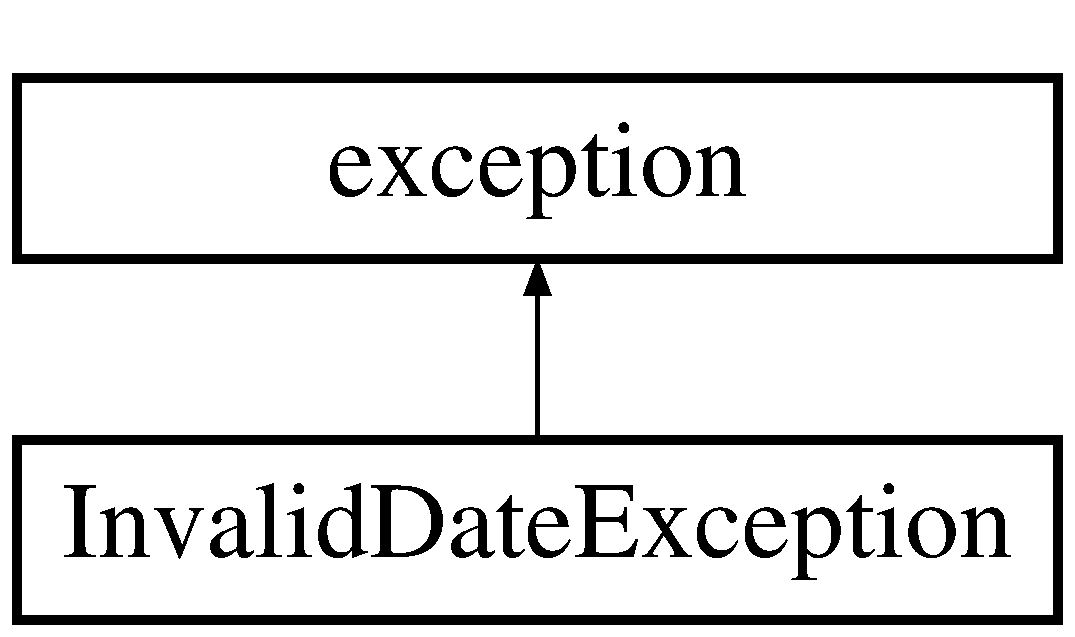
\includegraphics[height=3.000000cm]{classInvalidDateException}
\end{center}
\end{figure}
\subsection*{Public Member Functions}
\begin{DoxyCompactItemize}
\item 
\mbox{\Hypertarget{classInvalidDateException_a0ae7a8a97c0442fc025cb63e3b86bee8}\label{classInvalidDateException_a0ae7a8a97c0442fc025cb63e3b86bee8}} 
{\bfseries Invalid\+Date\+Exception} (std\+::string date\+String)
\item 
\mbox{\Hypertarget{classInvalidDateException_a518618417b66ea59ef6d5a40aad7d045}\label{classInvalidDateException_a518618417b66ea59ef6d5a40aad7d045}} 
std\+::string {\bfseries what} ()
\end{DoxyCompactItemize}
\subsection*{Public Attributes}
\begin{DoxyCompactItemize}
\item 
\mbox{\Hypertarget{classInvalidDateException_a70664a8f1fe8853eed11199c5c0f0060}\label{classInvalidDateException_a70664a8f1fe8853eed11199c5c0f0060}} 
std\+::string {\bfseries date\+String}
\end{DoxyCompactItemize}


The documentation for this class was generated from the following files\+:\begin{DoxyCompactItemize}
\item 
Invalid\+Date\+Exception.\+h\item 
Invalid\+Date\+Exception.\+cpp\end{DoxyCompactItemize}

\hypertarget{classInvalidTrainTypeException}{}\section{Invalid\+Train\+Type\+Exception Class Reference}
\label{classInvalidTrainTypeException}\index{Invalid\+Train\+Type\+Exception@{Invalid\+Train\+Type\+Exception}}


{\ttfamily \#include $<$Invalid\+Train\+Type\+Exception.\+h$>$}



Inheritance diagram for Invalid\+Train\+Type\+Exception\+:
\nopagebreak
\begin{figure}[H]
\begin{center}
\leavevmode
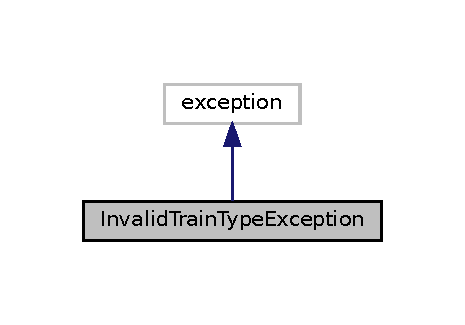
\includegraphics[width=223pt]{classInvalidTrainTypeException__inherit__graph}
\end{center}
\end{figure}


Collaboration diagram for Invalid\+Train\+Type\+Exception\+:
\nopagebreak
\begin{figure}[H]
\begin{center}
\leavevmode
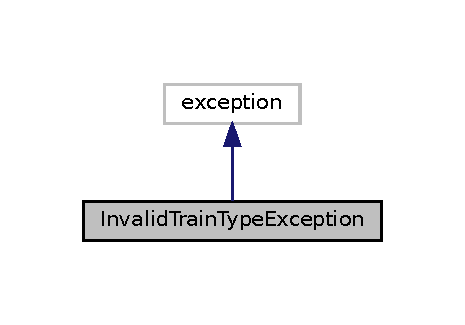
\includegraphics[width=223pt]{classInvalidTrainTypeException__coll__graph}
\end{center}
\end{figure}
\subsection*{Public Member Functions}
\begin{DoxyCompactItemize}
\item 
\mbox{\hyperlink{classInvalidTrainTypeException_aa06f57cd1c9c04bc98cece928a6f0ed8}{Invalid\+Train\+Type\+Exception}} (std\+::string type)
\item 
const char $\ast$ \mbox{\hyperlink{classInvalidTrainTypeException_a9eb95875231c7bace498e824f2e746c2}{what}} () const noexcept override
\end{DoxyCompactItemize}


\subsection{Detailed Description}
Exception reporting an invalid train type. 

\subsection{Constructor \& Destructor Documentation}
\mbox{\Hypertarget{classInvalidTrainTypeException_aa06f57cd1c9c04bc98cece928a6f0ed8}\label{classInvalidTrainTypeException_aa06f57cd1c9c04bc98cece928a6f0ed8}} 
\index{Invalid\+Train\+Type\+Exception@{Invalid\+Train\+Type\+Exception}!Invalid\+Train\+Type\+Exception@{Invalid\+Train\+Type\+Exception}}
\index{Invalid\+Train\+Type\+Exception@{Invalid\+Train\+Type\+Exception}!Invalid\+Train\+Type\+Exception@{Invalid\+Train\+Type\+Exception}}
\subsubsection{\texorpdfstring{Invalid\+Train\+Type\+Exception()}{InvalidTrainTypeException()}}
{\footnotesize\ttfamily Invalid\+Train\+Type\+Exception\+::\+Invalid\+Train\+Type\+Exception (\begin{DoxyParamCaption}\item[{std\+::string}]{type }\end{DoxyParamCaption})}



\subsection{Member Function Documentation}
\mbox{\Hypertarget{classInvalidTrainTypeException_a9eb95875231c7bace498e824f2e746c2}\label{classInvalidTrainTypeException_a9eb95875231c7bace498e824f2e746c2}} 
\index{Invalid\+Train\+Type\+Exception@{Invalid\+Train\+Type\+Exception}!what@{what}}
\index{what@{what}!Invalid\+Train\+Type\+Exception@{Invalid\+Train\+Type\+Exception}}
\subsubsection{\texorpdfstring{what()}{what()}}
{\footnotesize\ttfamily const char $\ast$ Invalid\+Train\+Type\+Exception\+::what (\begin{DoxyParamCaption}{ }\end{DoxyParamCaption}) const\hspace{0.3cm}{\ttfamily [override]}, {\ttfamily [noexcept]}}



The documentation for this class was generated from the following files\+:\begin{DoxyCompactItemize}
\item 
exceptions/\mbox{\hyperlink{InvalidTrainTypeException_8h}{Invalid\+Train\+Type\+Exception.\+h}}\item 
exceptions/\mbox{\hyperlink{InvalidTrainTypeException_8cpp}{Invalid\+Train\+Type\+Exception.\+cpp}}\end{DoxyCompactItemize}

\hypertarget{classNoSuchEngineerException}{}\section{No\+Such\+Engineer\+Exception Class Reference}
\label{classNoSuchEngineerException}\index{No\+Such\+Engineer\+Exception@{No\+Such\+Engineer\+Exception}}


{\ttfamily \#include $<$No\+Such\+Engineer\+Exception.\+h$>$}



Inheritance diagram for No\+Such\+Engineer\+Exception\+:
\nopagebreak
\begin{figure}[H]
\begin{center}
\leavevmode
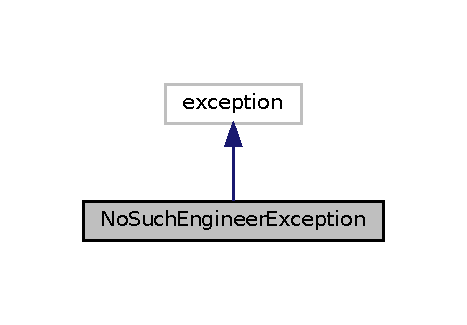
\includegraphics[width=224pt]{classNoSuchEngineerException__inherit__graph}
\end{center}
\end{figure}


Collaboration diagram for No\+Such\+Engineer\+Exception\+:
\nopagebreak
\begin{figure}[H]
\begin{center}
\leavevmode
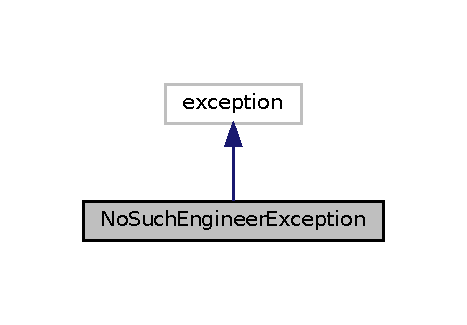
\includegraphics[width=224pt]{classNoSuchEngineerException__coll__graph}
\end{center}
\end{figure}
\subsection*{Public Member Functions}
\begin{DoxyCompactItemize}
\item 
\mbox{\hyperlink{classNoSuchEngineerException_acb7d95771ea1961a2cf223d3fcedd78a}{No\+Such\+Engineer\+Exception}} (\mbox{\hyperlink{project__utils_8h_a8f3a969054ad2200720b96e7e23dd4e1}{id\+\_\+t}} id)
\item 
const char $\ast$ \mbox{\hyperlink{classNoSuchEngineerException_a8d08bc83799855bed5d9ba2fddb56b34}{what}} ()
\end{DoxyCompactItemize}


\subsection{Detailed Description}
Exception reporting a non existing engineer id. 

\subsection{Constructor \& Destructor Documentation}
\mbox{\Hypertarget{classNoSuchEngineerException_acb7d95771ea1961a2cf223d3fcedd78a}\label{classNoSuchEngineerException_acb7d95771ea1961a2cf223d3fcedd78a}} 
\index{No\+Such\+Engineer\+Exception@{No\+Such\+Engineer\+Exception}!No\+Such\+Engineer\+Exception@{No\+Such\+Engineer\+Exception}}
\index{No\+Such\+Engineer\+Exception@{No\+Such\+Engineer\+Exception}!No\+Such\+Engineer\+Exception@{No\+Such\+Engineer\+Exception}}
\subsubsection{\texorpdfstring{No\+Such\+Engineer\+Exception()}{NoSuchEngineerException()}}
{\footnotesize\ttfamily No\+Such\+Engineer\+Exception\+::\+No\+Such\+Engineer\+Exception (\begin{DoxyParamCaption}\item[{\mbox{\hyperlink{project__utils_8h_a8f3a969054ad2200720b96e7e23dd4e1}{id\+\_\+t}}}]{id }\end{DoxyParamCaption})\hspace{0.3cm}{\ttfamily [explicit]}}



\subsection{Member Function Documentation}
\mbox{\Hypertarget{classNoSuchEngineerException_a8d08bc83799855bed5d9ba2fddb56b34}\label{classNoSuchEngineerException_a8d08bc83799855bed5d9ba2fddb56b34}} 
\index{No\+Such\+Engineer\+Exception@{No\+Such\+Engineer\+Exception}!what@{what}}
\index{what@{what}!No\+Such\+Engineer\+Exception@{No\+Such\+Engineer\+Exception}}
\subsubsection{\texorpdfstring{what()}{what()}}
{\footnotesize\ttfamily const char $\ast$ No\+Such\+Engineer\+Exception\+::what (\begin{DoxyParamCaption}{ }\end{DoxyParamCaption})}



The documentation for this class was generated from the following files\+:\begin{DoxyCompactItemize}
\item 
exceptions/\mbox{\hyperlink{NoSuchEngineerException_8h}{No\+Such\+Engineer\+Exception.\+h}}\item 
exceptions/\mbox{\hyperlink{NoSuchEngineerException_8cpp}{No\+Such\+Engineer\+Exception.\+cpp}}\end{DoxyCompactItemize}

\hypertarget{classNoSuchPassengerException}{}\section{No\+Such\+Passenger\+Exception Class Reference}
\label{classNoSuchPassengerException}\index{No\+Such\+Passenger\+Exception@{No\+Such\+Passenger\+Exception}}


Exception reporting that a passenger ID does not exist in the system.  




{\ttfamily \#include $<$No\+Such\+Passenger\+Exception.\+h$>$}

Inheritance diagram for No\+Such\+Passenger\+Exception\+:\begin{figure}[H]
\begin{center}
\leavevmode
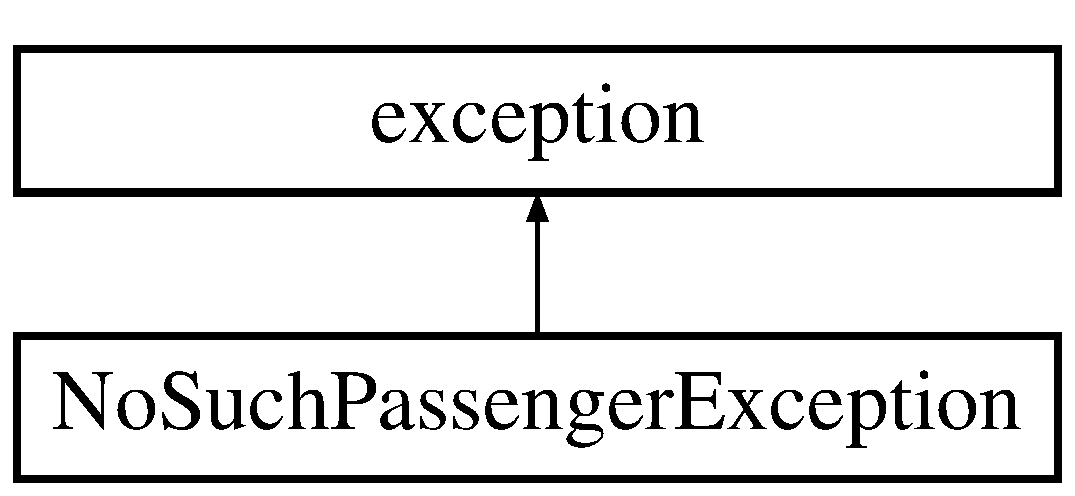
\includegraphics[height=3.000000cm]{classNoSuchPassengerException}
\end{center}
\end{figure}
\subsection*{Public Member Functions}
\begin{DoxyCompactItemize}
\item 
\mbox{\Hypertarget{classNoSuchPassengerException_a592e57495c93657a25e7da49da5b6649}\label{classNoSuchPassengerException_a592e57495c93657a25e7da49da5b6649}} 
{\bfseries No\+Such\+Passenger\+Exception} (id\+\_\+t id)
\item 
\mbox{\Hypertarget{classNoSuchPassengerException_a27bf9b4347fee63ddc405d58d217d82e}\label{classNoSuchPassengerException_a27bf9b4347fee63ddc405d58d217d82e}} 
std\+::string {\bfseries what} ()
\end{DoxyCompactItemize}


\subsection{Detailed Description}
Exception reporting that a passenger ID does not exist in the system. 

The documentation for this class was generated from the following files\+:\begin{DoxyCompactItemize}
\item 
No\+Such\+Passenger\+Exception.\+h\item 
No\+Such\+Passenger\+Exception.\+cpp\end{DoxyCompactItemize}

\hypertarget{classNoSuchStationException}{}\section{No\+Such\+Station\+Exception Class Reference}
\label{classNoSuchStationException}\index{No\+Such\+Station\+Exception@{No\+Such\+Station\+Exception}}
Inheritance diagram for No\+Such\+Station\+Exception\+:\begin{figure}[H]
\begin{center}
\leavevmode
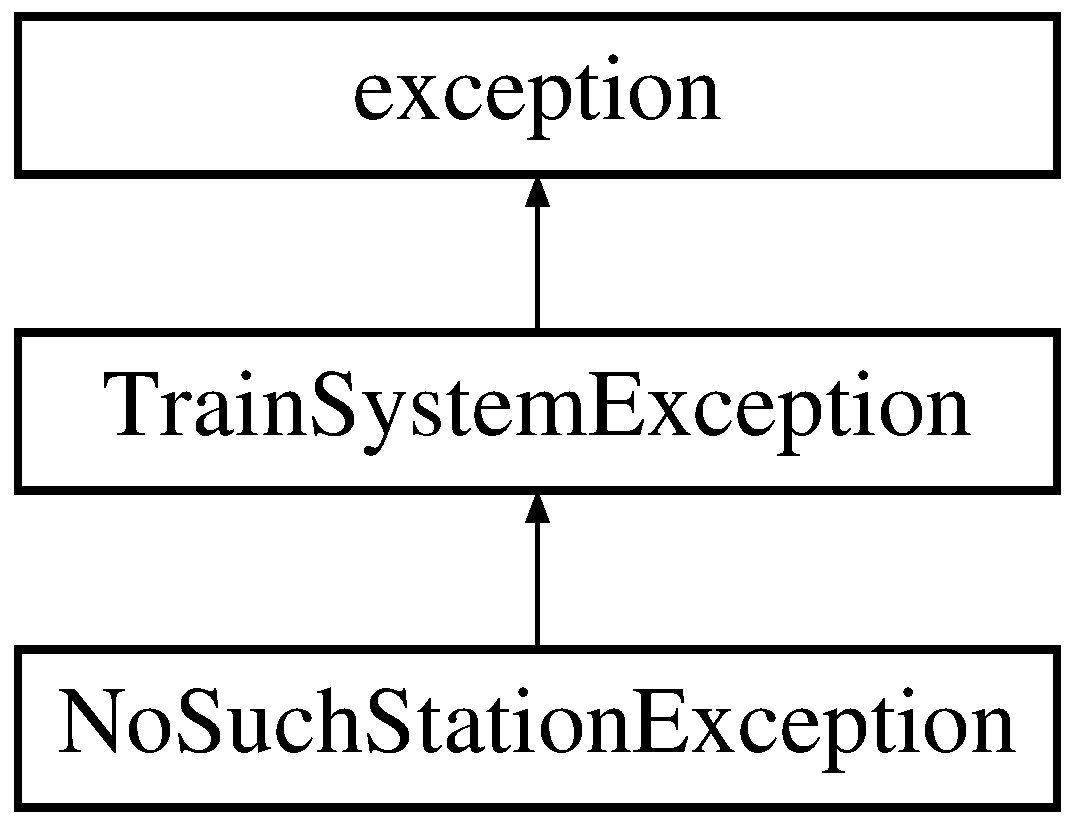
\includegraphics[height=3.000000cm]{classNoSuchStationException}
\end{center}
\end{figure}
\subsection*{Public Member Functions}
\begin{DoxyCompactItemize}
\item 
\mbox{\Hypertarget{classNoSuchStationException_a3e907e61f0836f6954f40bd63538bcb6}\label{classNoSuchStationException_a3e907e61f0836f6954f40bd63538bcb6}} 
{\bfseries No\+Such\+Station\+Exception} (id\+\_\+t id)
\item 
\mbox{\Hypertarget{classNoSuchStationException_aef7808e1393d0ed22d130fa05d20d8f7}\label{classNoSuchStationException_aef7808e1393d0ed22d130fa05d20d8f7}} 
std\+::string {\bfseries what} ()
\end{DoxyCompactItemize}


The documentation for this class was generated from the following files\+:\begin{DoxyCompactItemize}
\item 
No\+Such\+Station\+Exception.\+h\item 
No\+Such\+Station\+Exception.\+cpp\end{DoxyCompactItemize}

\hypertarget{classNoSuchTrainException}{}\section{No\+Such\+Train\+Exception Class Reference}
\label{classNoSuchTrainException}\index{No\+Such\+Train\+Exception@{No\+Such\+Train\+Exception}}


Exception reporting that a train ID does not exist in the system.  




{\ttfamily \#include $<$No\+Such\+Train\+Exception.\+h$>$}

Inheritance diagram for No\+Such\+Train\+Exception\+:\begin{figure}[H]
\begin{center}
\leavevmode
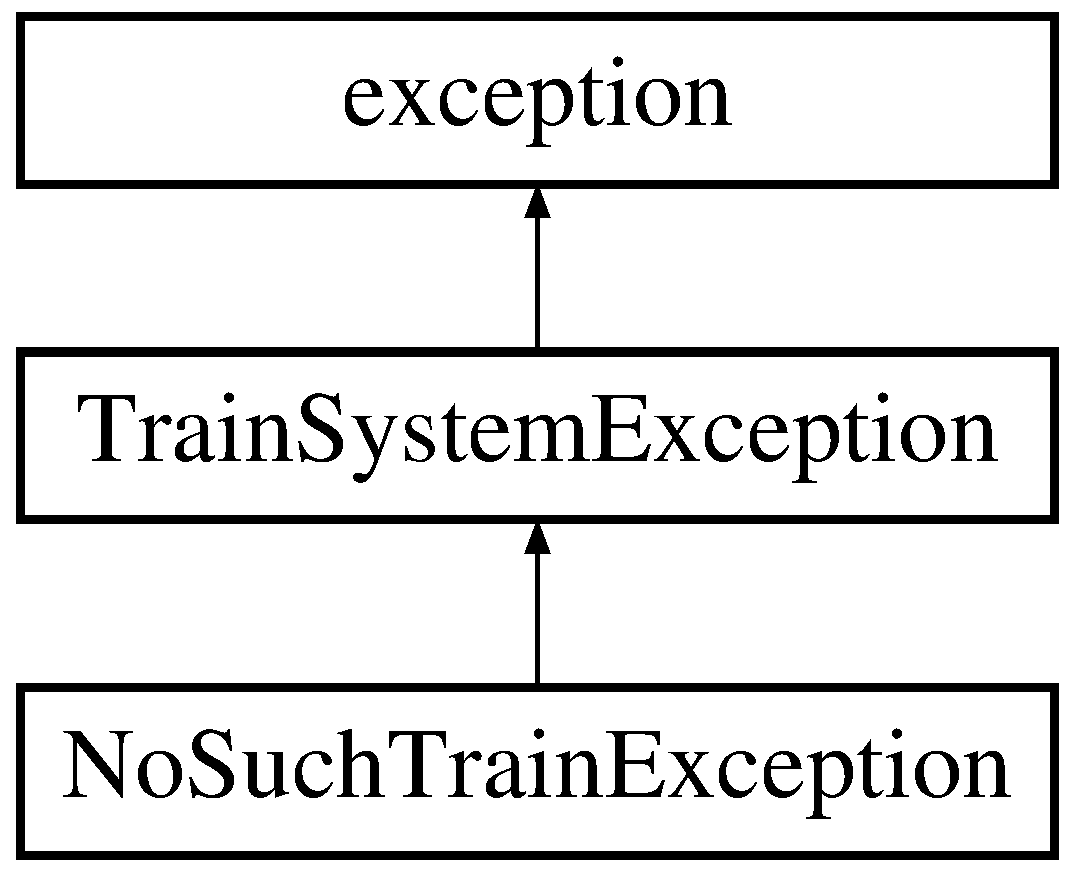
\includegraphics[height=3.000000cm]{classNoSuchTrainException}
\end{center}
\end{figure}
\subsection*{Public Member Functions}
\begin{DoxyCompactItemize}
\item 
\mbox{\Hypertarget{classNoSuchTrainException_ae60439498bd6e552159ed1c50335daba}\label{classNoSuchTrainException_ae60439498bd6e552159ed1c50335daba}} 
{\bfseries No\+Such\+Train\+Exception} (id\+\_\+t id)
\item 
\mbox{\Hypertarget{classNoSuchTrainException_a812ae27b54620f59e0a9e23969935099}\label{classNoSuchTrainException_a812ae27b54620f59e0a9e23969935099}} 
std\+::string {\bfseries what} ()
\end{DoxyCompactItemize}


\subsection{Detailed Description}
Exception reporting that a train ID does not exist in the system. 

The documentation for this class was generated from the following files\+:\begin{DoxyCompactItemize}
\item 
No\+Such\+Train\+Exception.\+h\item 
No\+Such\+Train\+Exception.\+cpp\end{DoxyCompactItemize}

\hypertarget{classNoSuchTripException}{}\section{No\+Such\+Trip\+Exception Class Reference}
\label{classNoSuchTripException}\index{No\+Such\+Trip\+Exception@{No\+Such\+Trip\+Exception}}


Exception reporting that a trip ID does not exist in the system.  




{\ttfamily \#include $<$No\+Such\+Trip\+Exception.\+h$>$}



Inheritance diagram for No\+Such\+Trip\+Exception\+:
\nopagebreak
\begin{figure}[H]
\begin{center}
\leavevmode
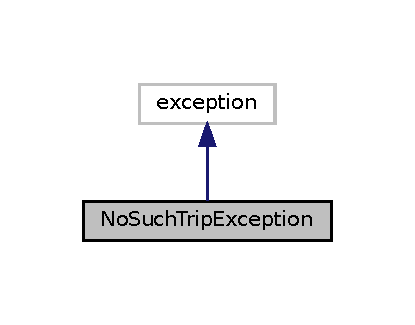
\includegraphics[width=199pt]{classNoSuchTripException__inherit__graph}
\end{center}
\end{figure}


Collaboration diagram for No\+Such\+Trip\+Exception\+:
\nopagebreak
\begin{figure}[H]
\begin{center}
\leavevmode
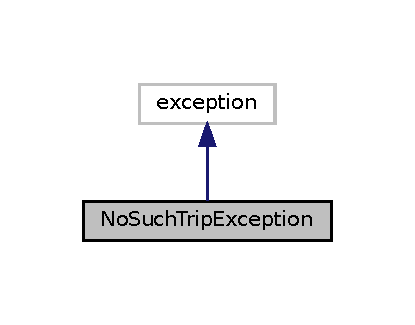
\includegraphics[width=199pt]{classNoSuchTripException__coll__graph}
\end{center}
\end{figure}
\subsection*{Public Member Functions}
\begin{DoxyCompactItemize}
\item 
\mbox{\hyperlink{classNoSuchTripException_ad4e2e75706508833ccbb7a793092734c}{No\+Such\+Trip\+Exception}} (\mbox{\hyperlink{project__utils_8h_a8f3a969054ad2200720b96e7e23dd4e1}{id\+\_\+t}} id)
\item 
const char $\ast$ \mbox{\hyperlink{classNoSuchTripException_a48adffc40883e044fd248f1185084bb6}{what}} ()
\end{DoxyCompactItemize}


\subsection{Detailed Description}
Exception reporting that a trip ID does not exist in the system. 

\subsection{Constructor \& Destructor Documentation}
\mbox{\Hypertarget{classNoSuchTripException_ad4e2e75706508833ccbb7a793092734c}\label{classNoSuchTripException_ad4e2e75706508833ccbb7a793092734c}} 
\index{No\+Such\+Trip\+Exception@{No\+Such\+Trip\+Exception}!No\+Such\+Trip\+Exception@{No\+Such\+Trip\+Exception}}
\index{No\+Such\+Trip\+Exception@{No\+Such\+Trip\+Exception}!No\+Such\+Trip\+Exception@{No\+Such\+Trip\+Exception}}
\subsubsection{\texorpdfstring{No\+Such\+Trip\+Exception()}{NoSuchTripException()}}
{\footnotesize\ttfamily No\+Such\+Trip\+Exception\+::\+No\+Such\+Trip\+Exception (\begin{DoxyParamCaption}\item[{\mbox{\hyperlink{project__utils_8h_a8f3a969054ad2200720b96e7e23dd4e1}{id\+\_\+t}}}]{id }\end{DoxyParamCaption})}



\subsection{Member Function Documentation}
\mbox{\Hypertarget{classNoSuchTripException_a48adffc40883e044fd248f1185084bb6}\label{classNoSuchTripException_a48adffc40883e044fd248f1185084bb6}} 
\index{No\+Such\+Trip\+Exception@{No\+Such\+Trip\+Exception}!what@{what}}
\index{what@{what}!No\+Such\+Trip\+Exception@{No\+Such\+Trip\+Exception}}
\subsubsection{\texorpdfstring{what()}{what()}}
{\footnotesize\ttfamily const char $\ast$ No\+Such\+Trip\+Exception\+::what (\begin{DoxyParamCaption}{ }\end{DoxyParamCaption})}



The documentation for this class was generated from the following files\+:\begin{DoxyCompactItemize}
\item 
exceptions/\mbox{\hyperlink{NoSuchTripException_8h}{No\+Such\+Trip\+Exception.\+h}}\item 
exceptions/\mbox{\hyperlink{NoSuchTripException_8cpp}{No\+Such\+Trip\+Exception.\+cpp}}\end{DoxyCompactItemize}

\hypertarget{classPassenger}{}\section{Passenger Class Reference}
\label{classPassenger}\index{Passenger@{Passenger}}
\subsection*{Public Member Functions}
\begin{DoxyCompactItemize}
\item 
\mbox{\Hypertarget{classPassenger_a895d7a9cfd358b566ed78e0d81d37bff}\label{classPassenger_a895d7a9cfd358b566ed78e0d81d37bff}} 
{\bfseries Passenger} (std\+::string name, std\+::string birth\+Date)
\item 
\mbox{\Hypertarget{classPassenger_ae6fcc19037be144f654c623c5b78ae24}\label{classPassenger_ae6fcc19037be144f654c623c5b78ae24}} 
id\+\_\+t {\bfseries get\+ID} () const
\item 
\mbox{\Hypertarget{classPassenger_a7c919f6947817ff1c6a4ee51923c116f}\label{classPassenger_a7c919f6947817ff1c6a4ee51923c116f}} 
std\+::string {\bfseries get\+Name} () const
\item 
\mbox{\Hypertarget{classPassenger_ae8d5310db80438702dec5f4d649289f1}\label{classPassenger_ae8d5310db80438702dec5f4d649289f1}} 
\mbox{\hyperlink{classPassengerCard}{Passenger\+Card}} $\ast$ {\bfseries get\+Card} () const
\item 
\mbox{\Hypertarget{classPassenger_aa2101584d2f0daf83ef58e0491754395}\label{classPassenger_aa2101584d2f0daf83ef58e0491754395}} 
const \mbox{\hyperlink{classDate}{Date}} \& {\bfseries get\+Birth\+Date} () const
\item 
\mbox{\Hypertarget{classPassenger_a06dfa54524d4ca1a85b1599b278fb871}\label{classPassenger_a06dfa54524d4ca1a85b1599b278fb871}} 
const std\+::vector$<$ \mbox{\hyperlink{classTrip}{Trip}} $\ast$ $>$ \& {\bfseries get\+Trips} () const
\item 
\mbox{\Hypertarget{classPassenger_a2fef29e013c88ba7a75d259cebfa655d}\label{classPassenger_a2fef29e013c88ba7a75d259cebfa655d}} 
bool {\bfseries add\+Trip} (\mbox{\hyperlink{classTrip}{Trip}} $\ast$trip)
\item 
\mbox{\Hypertarget{classPassenger_a72e4042544557a3dd9c02198aa2582d8}\label{classPassenger_a72e4042544557a3dd9c02198aa2582d8}} 
void {\bfseries print\+Row} (std\+::ostream \&os)
\end{DoxyCompactItemize}
\subsection*{Friends}
\begin{DoxyCompactItemize}
\item 
\mbox{\Hypertarget{classPassenger_a7b1aeaded08562578690b788f39db888}\label{classPassenger_a7b1aeaded08562578690b788f39db888}} 
std\+::ostream \& {\bfseries operator$<$$<$} (std\+::ostream \&os, \mbox{\hyperlink{classPassenger}{Passenger}} \&p)
\end{DoxyCompactItemize}


The documentation for this class was generated from the following files\+:\begin{DoxyCompactItemize}
\item 
Passenger.\+h\item 
Passenger.\+cpp\end{DoxyCompactItemize}

\hypertarget{classPassengerCard}{}\section{Passenger\+Card Class Reference}
\label{classPassengerCard}\index{Passenger\+Card@{Passenger\+Card}}


Class for representing the card of a passenger in the system.  




{\ttfamily \#include $<$Passenger\+Card.\+h$>$}

\subsection*{Public Types}
\begin{DoxyCompactItemize}
\item 
enum \mbox{\hyperlink{classPassengerCard_ac30388c823af514403463a797e2878af}{Card\+Type}} \{ \mbox{\hyperlink{classPassengerCard_ac30388c823af514403463a797e2878afab0b85af6d5ffb07453865fc04cae9453}{twenty\+Five}} =25, 
\mbox{\hyperlink{classPassengerCard_ac30388c823af514403463a797e2878afac443f0b05b5c1f059e4a99fef0cdea4c}{fifty}} =50, 
\mbox{\hyperlink{classPassengerCard_ac30388c823af514403463a797e2878afaa1ae2020789a526d593e7b80d4ee370d}{hundred}} =100
 \}
\begin{DoxyCompactList}\small\item\em Card Type enum. \end{DoxyCompactList}\end{DoxyCompactItemize}
\subsection*{Public Member Functions}
\begin{DoxyCompactItemize}
\item 
\mbox{\hyperlink{classPassengerCard_a1ebc730da7c0820350024f29c37ce9d9}{Passenger\+Card}} (\mbox{\hyperlink{classPassengerCard_ac30388c823af514403463a797e2878af}{Card\+Type}} type, \mbox{\hyperlink{project__utils_8h_a8f3a969054ad2200720b96e7e23dd4e1}{id\+\_\+t}} passenger\+ID, std\+::string p\+Name)
\begin{DoxyCompactList}\small\item\em Construct a new \mbox{\hyperlink{classPassenger}{Passenger}} Card object. \end{DoxyCompactList}\item 
int \mbox{\hyperlink{classPassengerCard_a62d2651d233d28643d5e0863500c42c4}{get\+Discount}} () const
\begin{DoxyCompactList}\small\item\em Get the discount percentage provided by the card. \end{DoxyCompactList}\item 
\mbox{\hyperlink{classPassengerCard_ac30388c823af514403463a797e2878af}{Card\+Type}} \mbox{\hyperlink{classPassengerCard_aef682e4bb625ac937c4aec7999c92626}{get\+Type}} ()
\begin{DoxyCompactList}\small\item\em Get the Type object. \end{DoxyCompactList}\item 
\mbox{\hyperlink{project__utils_8h_a91ad9478d81a7aaf2593e8d9c3d06a14}{uint}} \mbox{\hyperlink{classPassengerCard_a8428ca4fc3d4c7b4636be628c2fe5aad}{get\+Cost}} ()
\begin{DoxyCompactList}\small\item\em Get the monthly cost of the card. \end{DoxyCompactList}\item 
void \mbox{\hyperlink{classPassengerCard_ab0c4c67f185dc1abee907b6cd50413bf}{set\+Type}} (\mbox{\hyperlink{classPassengerCard_ac30388c823af514403463a797e2878af}{Card\+Type}} type)
\begin{DoxyCompactList}\small\item\em Set the typeof the card. \end{DoxyCompactList}\end{DoxyCompactItemize}
\subsection*{Static Public Attributes}
\begin{DoxyCompactItemize}
\item 
static \mbox{\hyperlink{project__utils_8h_a8f3a969054ad2200720b96e7e23dd4e1}{id\+\_\+t}} \mbox{\hyperlink{classPassengerCard_af557a01fde14b95c0e0b355e777e2aec}{current\+ID}} = 0
\begin{DoxyCompactList}\small\item\em Next ID Counter. \end{DoxyCompactList}\end{DoxyCompactItemize}


\subsection{Detailed Description}
Class for representing the card of a passenger in the system. 

\subsection{Member Enumeration Documentation}
\mbox{\Hypertarget{classPassengerCard_ac30388c823af514403463a797e2878af}\label{classPassengerCard_ac30388c823af514403463a797e2878af}} 
\index{Passenger\+Card@{Passenger\+Card}!Card\+Type@{Card\+Type}}
\index{Card\+Type@{Card\+Type}!Passenger\+Card@{Passenger\+Card}}
\subsubsection{\texorpdfstring{Card\+Type}{CardType}}
{\footnotesize\ttfamily enum \mbox{\hyperlink{classPassengerCard_ac30388c823af514403463a797e2878af}{Passenger\+Card\+::\+Card\+Type}}}



Card Type enum. 

\begin{DoxyEnumFields}{Enumerator}
\raisebox{\heightof{T}}[0pt][0pt]{\index{twenty\+Five@{twenty\+Five}!Passenger\+Card@{Passenger\+Card}}\index{Passenger\+Card@{Passenger\+Card}!twenty\+Five@{twenty\+Five}}}\mbox{\Hypertarget{classPassengerCard_ac30388c823af514403463a797e2878afab0b85af6d5ffb07453865fc04cae9453}\label{classPassengerCard_ac30388c823af514403463a797e2878afab0b85af6d5ffb07453865fc04cae9453}} 
twenty\+Five&\\
\hline

\raisebox{\heightof{T}}[0pt][0pt]{\index{fifty@{fifty}!Passenger\+Card@{Passenger\+Card}}\index{Passenger\+Card@{Passenger\+Card}!fifty@{fifty}}}\mbox{\Hypertarget{classPassengerCard_ac30388c823af514403463a797e2878afac443f0b05b5c1f059e4a99fef0cdea4c}\label{classPassengerCard_ac30388c823af514403463a797e2878afac443f0b05b5c1f059e4a99fef0cdea4c}} 
fifty&\\
\hline

\raisebox{\heightof{T}}[0pt][0pt]{\index{hundred@{hundred}!Passenger\+Card@{Passenger\+Card}}\index{Passenger\+Card@{Passenger\+Card}!hundred@{hundred}}}\mbox{\Hypertarget{classPassengerCard_ac30388c823af514403463a797e2878afaa1ae2020789a526d593e7b80d4ee370d}\label{classPassengerCard_ac30388c823af514403463a797e2878afaa1ae2020789a526d593e7b80d4ee370d}} 
hundred&\\
\hline

\end{DoxyEnumFields}


\subsection{Constructor \& Destructor Documentation}
\mbox{\Hypertarget{classPassengerCard_a1ebc730da7c0820350024f29c37ce9d9}\label{classPassengerCard_a1ebc730da7c0820350024f29c37ce9d9}} 
\index{Passenger\+Card@{Passenger\+Card}!Passenger\+Card@{Passenger\+Card}}
\index{Passenger\+Card@{Passenger\+Card}!Passenger\+Card@{Passenger\+Card}}
\subsubsection{\texorpdfstring{Passenger\+Card()}{PassengerCard()}}
{\footnotesize\ttfamily Passenger\+Card\+::\+Passenger\+Card (\begin{DoxyParamCaption}\item[{\mbox{\hyperlink{classPassengerCard_ac30388c823af514403463a797e2878af}{Card\+Type}}}]{type,  }\item[{\mbox{\hyperlink{project__utils_8h_a8f3a969054ad2200720b96e7e23dd4e1}{id\+\_\+t}}}]{passenger\+ID,  }\item[{std\+::string}]{p\+Name }\end{DoxyParamCaption})}



Construct a new \mbox{\hyperlink{classPassenger}{Passenger}} Card object. 


\begin{DoxyParams}{Parameters}
{\em type} & Type of the card \\
\hline
{\em passenger\+ID} & ID of the passenger \\
\hline
{\em p\+Name} & Name of the passenger that owns the card \\
\hline
\end{DoxyParams}


\subsection{Member Function Documentation}
\mbox{\Hypertarget{classPassengerCard_a8428ca4fc3d4c7b4636be628c2fe5aad}\label{classPassengerCard_a8428ca4fc3d4c7b4636be628c2fe5aad}} 
\index{Passenger\+Card@{Passenger\+Card}!get\+Cost@{get\+Cost}}
\index{get\+Cost@{get\+Cost}!Passenger\+Card@{Passenger\+Card}}
\subsubsection{\texorpdfstring{get\+Cost()}{getCost()}}
{\footnotesize\ttfamily \mbox{\hyperlink{project__utils_8h_a91ad9478d81a7aaf2593e8d9c3d06a14}{uint}} Passenger\+Card\+::get\+Cost (\begin{DoxyParamCaption}{ }\end{DoxyParamCaption})}



Get the monthly cost of the card. 

\begin{DoxyReturn}{Returns}
uint Monthly cost of the card in cents 
\end{DoxyReturn}
\mbox{\Hypertarget{classPassengerCard_a62d2651d233d28643d5e0863500c42c4}\label{classPassengerCard_a62d2651d233d28643d5e0863500c42c4}} 
\index{Passenger\+Card@{Passenger\+Card}!get\+Discount@{get\+Discount}}
\index{get\+Discount@{get\+Discount}!Passenger\+Card@{Passenger\+Card}}
\subsubsection{\texorpdfstring{get\+Discount()}{getDiscount()}}
{\footnotesize\ttfamily int Passenger\+Card\+::get\+Discount (\begin{DoxyParamCaption}{ }\end{DoxyParamCaption}) const}



Get the discount percentage provided by the card. 

\begin{DoxyReturn}{Returns}
int Percentag of discount 
\end{DoxyReturn}
\mbox{\Hypertarget{classPassengerCard_aef682e4bb625ac937c4aec7999c92626}\label{classPassengerCard_aef682e4bb625ac937c4aec7999c92626}} 
\index{Passenger\+Card@{Passenger\+Card}!get\+Type@{get\+Type}}
\index{get\+Type@{get\+Type}!Passenger\+Card@{Passenger\+Card}}
\subsubsection{\texorpdfstring{get\+Type()}{getType()}}
{\footnotesize\ttfamily \mbox{\hyperlink{classPassengerCard_ac30388c823af514403463a797e2878af}{Passenger\+Card\+::\+Card\+Type}} Passenger\+Card\+::get\+Type (\begin{DoxyParamCaption}{ }\end{DoxyParamCaption})}



Get the Type object. 

\begin{DoxyReturn}{Returns}
Card\+Type 
\end{DoxyReturn}
\mbox{\Hypertarget{classPassengerCard_ab0c4c67f185dc1abee907b6cd50413bf}\label{classPassengerCard_ab0c4c67f185dc1abee907b6cd50413bf}} 
\index{Passenger\+Card@{Passenger\+Card}!set\+Type@{set\+Type}}
\index{set\+Type@{set\+Type}!Passenger\+Card@{Passenger\+Card}}
\subsubsection{\texorpdfstring{set\+Type()}{setType()}}
{\footnotesize\ttfamily void Passenger\+Card\+::set\+Type (\begin{DoxyParamCaption}\item[{\mbox{\hyperlink{classPassengerCard_ac30388c823af514403463a797e2878af}{Card\+Type}}}]{type }\end{DoxyParamCaption})}



Set the typeof the card. 


\begin{DoxyParams}{Parameters}
{\em type} & \\
\hline
\end{DoxyParams}


\subsection{Member Data Documentation}
\mbox{\Hypertarget{classPassengerCard_af557a01fde14b95c0e0b355e777e2aec}\label{classPassengerCard_af557a01fde14b95c0e0b355e777e2aec}} 
\index{Passenger\+Card@{Passenger\+Card}!current\+ID@{current\+ID}}
\index{current\+ID@{current\+ID}!Passenger\+Card@{Passenger\+Card}}
\subsubsection{\texorpdfstring{current\+ID}{currentID}}
{\footnotesize\ttfamily \mbox{\hyperlink{project__utils_8h_a8f3a969054ad2200720b96e7e23dd4e1}{id\+\_\+t}} Passenger\+Card\+::current\+ID = 0\hspace{0.3cm}{\ttfamily [static]}}



Next ID Counter. 

Used to set new ID when \mbox{\hyperlink{classPassengerCard}{Passenger\+Card}} object is constructed, incremented every time a new \mbox{\hyperlink{classPassengerCard}{Passenger\+Card}} object is constructed. 

The documentation for this class was generated from the following files\+:\begin{DoxyCompactItemize}
\item 
system\+\_\+elements/\mbox{\hyperlink{PassengerCard_8h}{Passenger\+Card.\+h}}\item 
system\+\_\+elements/\mbox{\hyperlink{PassengerCard_8cpp}{Passenger\+Card.\+cpp}}\end{DoxyCompactItemize}

\hypertarget{classPerson}{}\section{Person Class Reference}
\label{classPerson}\index{Person@{Person}}


{\ttfamily \#include $<$Person.\+h$>$}



Inheritance diagram for Person\+:
\nopagebreak
\begin{figure}[H]
\begin{center}
\leavevmode
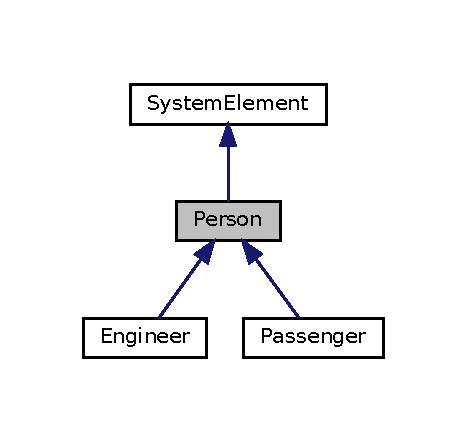
\includegraphics[width=224pt]{classPerson__inherit__graph}
\end{center}
\end{figure}


Collaboration diagram for Person\+:
\nopagebreak
\begin{figure}[H]
\begin{center}
\leavevmode
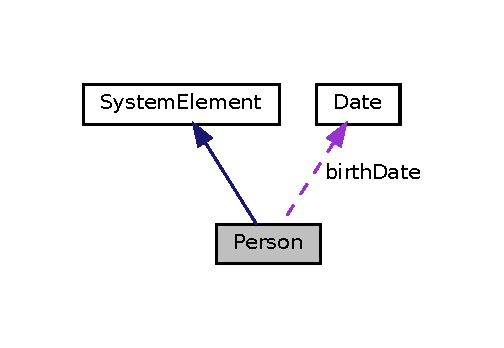
\includegraphics[width=242pt]{classPerson__coll__graph}
\end{center}
\end{figure}
\subsection*{Public Member Functions}
\begin{DoxyCompactItemize}
\item 
\mbox{\hyperlink{classPerson_aa4fc660ce27df46986187ce76481f126}{Person}} (std\+::string \mbox{\hyperlink{classPerson_a7594663aadc0de77616506df8a2f4128}{name}}, \mbox{\hyperlink{classDate}{Date}} \mbox{\hyperlink{classPerson_a7a764b56b815321eeb8412c1dcc4cabf}{birth\+Date}})
\item 
std\+::string \mbox{\hyperlink{classPerson_ab20f096fdfd5201818c45754af4c3e3b}{get\+Name}} () const
\begin{DoxyCompactList}\small\item\em Get the person\textquotesingle{}s name. \end{DoxyCompactList}\item 
\mbox{\hyperlink{classDate}{Date}} \& \mbox{\hyperlink{classPerson_a9f24821cb33c10e512eee2a5ad09c920}{get\+Birth\+Date}} ()
\begin{DoxyCompactList}\small\item\em Get the person\textquotesingle{}s Birth \mbox{\hyperlink{classDate}{Date}}. \end{DoxyCompactList}\end{DoxyCompactItemize}
\subsection*{Protected Attributes}
\begin{DoxyCompactItemize}
\item 
std\+::string \mbox{\hyperlink{classPerson_a7594663aadc0de77616506df8a2f4128}{name}}
\begin{DoxyCompactList}\small\item\em \mbox{\hyperlink{classPerson}{Person}}\textquotesingle{}s name. \end{DoxyCompactList}\item 
\mbox{\hyperlink{classDate}{Date}} \mbox{\hyperlink{classPerson_a7a764b56b815321eeb8412c1dcc4cabf}{birth\+Date}}
\begin{DoxyCompactList}\small\item\em \mbox{\hyperlink{classDate}{Date}} object representing \mbox{\hyperlink{classPassenger}{Passenger}}\textquotesingle{}s date of birth. \end{DoxyCompactList}\end{DoxyCompactItemize}


\subsection{Detailed Description}
Class representing a person in the \mbox{\hyperlink{classSystem}{System}}. 

\subsection{Constructor \& Destructor Documentation}
\mbox{\Hypertarget{classPerson_aa4fc660ce27df46986187ce76481f126}\label{classPerson_aa4fc660ce27df46986187ce76481f126}} 
\index{Person@{Person}!Person@{Person}}
\index{Person@{Person}!Person@{Person}}
\subsubsection{\texorpdfstring{Person()}{Person()}}
{\footnotesize\ttfamily Person\+::\+Person (\begin{DoxyParamCaption}\item[{std\+::string}]{name,  }\item[{\mbox{\hyperlink{classDate}{Date}}}]{birth\+Date }\end{DoxyParamCaption})}



\subsection{Member Function Documentation}
\mbox{\Hypertarget{classPerson_a9f24821cb33c10e512eee2a5ad09c920}\label{classPerson_a9f24821cb33c10e512eee2a5ad09c920}} 
\index{Person@{Person}!get\+Birth\+Date@{get\+Birth\+Date}}
\index{get\+Birth\+Date@{get\+Birth\+Date}!Person@{Person}}
\subsubsection{\texorpdfstring{get\+Birth\+Date()}{getBirthDate()}}
{\footnotesize\ttfamily \mbox{\hyperlink{classDate}{Date}} \& Person\+::get\+Birth\+Date (\begin{DoxyParamCaption}{ }\end{DoxyParamCaption})}



Get the person\textquotesingle{}s Birth \mbox{\hyperlink{classDate}{Date}}. 

\begin{DoxyReturn}{Returns}
const \mbox{\hyperlink{classDate}{Date}}\& The \mbox{\hyperlink{classDate}{Date}} object representing the \mbox{\hyperlink{classPassenger}{Passenger}}\textquotesingle{}s date of birth 
\end{DoxyReturn}
\mbox{\Hypertarget{classPerson_ab20f096fdfd5201818c45754af4c3e3b}\label{classPerson_ab20f096fdfd5201818c45754af4c3e3b}} 
\index{Person@{Person}!get\+Name@{get\+Name}}
\index{get\+Name@{get\+Name}!Person@{Person}}
\subsubsection{\texorpdfstring{get\+Name()}{getName()}}
{\footnotesize\ttfamily std\+::string Person\+::get\+Name (\begin{DoxyParamCaption}{ }\end{DoxyParamCaption}) const}



Get the person\textquotesingle{}s name. 

\begin{DoxyReturn}{Returns}
std\+::string The person\textquotesingle{}s name 
\end{DoxyReturn}


\subsection{Member Data Documentation}
\mbox{\Hypertarget{classPerson_a7a764b56b815321eeb8412c1dcc4cabf}\label{classPerson_a7a764b56b815321eeb8412c1dcc4cabf}} 
\index{Person@{Person}!birth\+Date@{birth\+Date}}
\index{birth\+Date@{birth\+Date}!Person@{Person}}
\subsubsection{\texorpdfstring{birth\+Date}{birthDate}}
{\footnotesize\ttfamily \mbox{\hyperlink{classDate}{Date}} Person\+::birth\+Date\hspace{0.3cm}{\ttfamily [protected]}}



\mbox{\hyperlink{classDate}{Date}} object representing \mbox{\hyperlink{classPassenger}{Passenger}}\textquotesingle{}s date of birth. 

\mbox{\Hypertarget{classPerson_a7594663aadc0de77616506df8a2f4128}\label{classPerson_a7594663aadc0de77616506df8a2f4128}} 
\index{Person@{Person}!name@{name}}
\index{name@{name}!Person@{Person}}
\subsubsection{\texorpdfstring{name}{name}}
{\footnotesize\ttfamily std\+::string Person\+::name\hspace{0.3cm}{\ttfamily [protected]}}



\mbox{\hyperlink{classPerson}{Person}}\textquotesingle{}s name. 



The documentation for this class was generated from the following files\+:\begin{DoxyCompactItemize}
\item 
system\+\_\+elements/\mbox{\hyperlink{Person_8h}{Person.\+h}}\item 
system\+\_\+elements/\mbox{\hyperlink{Person_8cpp}{Person.\+cpp}}\end{DoxyCompactItemize}

\hypertarget{classPurchaseLog}{}\section{Purchase\+Log Class Reference}
\label{classPurchaseLog}\index{Purchase\+Log@{Purchase\+Log}}
\subsection*{Public Member Functions}
\begin{DoxyCompactItemize}
\item 
\mbox{\Hypertarget{classPurchaseLog_a506a4e57eb23f36769c5dee6a4ec6fa0}\label{classPurchaseLog_a506a4e57eb23f36769c5dee6a4ec6fa0}} 
{\bfseries Purchase\+Log} (std\+::string passenger\+Name, std\+::string source\+Name, std\+::string dest\+Name, std\+::string departure\+Date, std\+::string price)
\item 
\mbox{\Hypertarget{classPurchaseLog_a0320e9136e01de2a9652db55c1739d6f}\label{classPurchaseLog_a0320e9136e01de2a9652db55c1739d6f}} 
const id\+\_\+t {\bfseries get\+ID} () const
\item 
\mbox{\Hypertarget{classPurchaseLog_a53f354f530d3179139eff0dbcf7aa67b}\label{classPurchaseLog_a53f354f530d3179139eff0dbcf7aa67b}} 
const std\+::string {\bfseries get\+Passenger\+Name} () const
\item 
\mbox{\Hypertarget{classPurchaseLog_a5c994361a33f18ad521a2af034a6cd8f}\label{classPurchaseLog_a5c994361a33f18ad521a2af034a6cd8f}} 
const std\+::string {\bfseries get\+Source\+Name} () const
\item 
\mbox{\Hypertarget{classPurchaseLog_a1ced321455e51202b4fbc962a2ab4398}\label{classPurchaseLog_a1ced321455e51202b4fbc962a2ab4398}} 
const std\+::string {\bfseries get\+Dest\+Name} () const
\item 
\mbox{\Hypertarget{classPurchaseLog_a55fd3400a7c03a09a276bfc015f75415}\label{classPurchaseLog_a55fd3400a7c03a09a276bfc015f75415}} 
const std\+::string {\bfseries get\+Departure\+Date} () const
\item 
\mbox{\Hypertarget{classPurchaseLog_a5fc1010f824f9ce26c309f9682d1b5ff}\label{classPurchaseLog_a5fc1010f824f9ce26c309f9682d1b5ff}} 
const std\+::string {\bfseries get\+Price} () const
\end{DoxyCompactItemize}
\subsection*{Static Public Attributes}
\begin{DoxyCompactItemize}
\item 
\mbox{\Hypertarget{classPurchaseLog_a175b76f4fd112806badc0ea294bccca5}\label{classPurchaseLog_a175b76f4fd112806badc0ea294bccca5}} 
static id\+\_\+t {\bfseries current\+Id} = 0
\end{DoxyCompactItemize}
\subsection*{Friends}
\begin{DoxyCompactItemize}
\item 
\mbox{\Hypertarget{classPurchaseLog_a49c8f4f31115140c5700334bd9933525}\label{classPurchaseLog_a49c8f4f31115140c5700334bd9933525}} 
std\+::ostream \& {\bfseries operator$<$$<$} (std\+::ostream \&os, \mbox{\hyperlink{classPurchaseLog}{Purchase\+Log}} \&pl)
\end{DoxyCompactItemize}


The documentation for this class was generated from the following files\+:\begin{DoxyCompactItemize}
\item 
Purchase\+Log.\+h\item 
Purchase\+Log.\+cpp\end{DoxyCompactItemize}

\hypertarget{classRepairShop}{}\section{Repair\+Shop Class Reference}
\label{classRepairShop}\index{Repair\+Shop@{Repair\+Shop}}


{\ttfamily \#include $<$Repair\+Shop.\+h$>$}



Inheritance diagram for Repair\+Shop\+:
\nopagebreak
\begin{figure}[H]
\begin{center}
\leavevmode
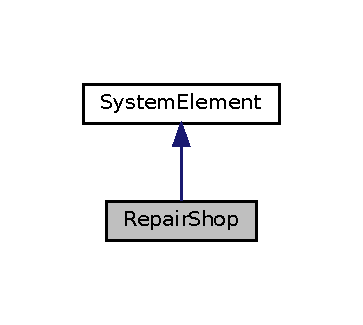
\includegraphics[width=174pt]{classRepairShop__inherit__graph}
\end{center}
\end{figure}


Collaboration diagram for Repair\+Shop\+:
\nopagebreak
\begin{figure}[H]
\begin{center}
\leavevmode
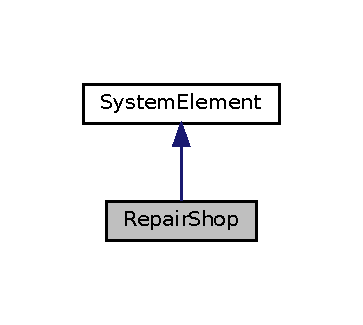
\includegraphics[width=174pt]{classRepairShop__coll__graph}
\end{center}
\end{figure}
\subsection*{Classes}
\begin{DoxyCompactItemize}
\item 
struct \mbox{\hyperlink{structRepairShop_1_1RepairShopPQUtils}{Repair\+Shop\+P\+Q\+Utils}}
\end{DoxyCompactItemize}
\subsection*{Public Member Functions}
\begin{DoxyCompactItemize}
\item 
\mbox{\hyperlink{classRepairShop_adb1c691ca60133e5e95a7d06489854e6}{Repair\+Shop}} (std\+::string \&name, int x, int y)
\item 
void \mbox{\hyperlink{classRepairShop_ab3b24779f3d3bf3b9e9a70f1a4cb78c5}{set\+ID}} (\mbox{\hyperlink{project__utils_8h_a8f3a969054ad2200720b96e7e23dd4e1}{id\+\_\+t}} id)
\item 
\mbox{\hyperlink{project__utils_8h_a8f3a969054ad2200720b96e7e23dd4e1}{id\+\_\+t}} \mbox{\hyperlink{classRepairShop_a78f871f65f7bf4b0f068b9406998f351}{get\+ID}} () const
\item 
int \mbox{\hyperlink{classRepairShop_ae0def7ba65f30ff9e7ddc0228c5b7ef8}{get\+Days\+To\+Availability}} () const
\item 
const string \& \mbox{\hyperlink{classRepairShop_ae470c339746dcb9ba5bb4c58195e0400}{get\+Name}} () const
\item 
int \mbox{\hyperlink{classRepairShop_a5a1fe514136f22f66e8676421525c896}{get\+X\+Coord}} () const
\item 
int \mbox{\hyperlink{classRepairShop_a9c3c6369451f7da751ca1c6845d5d8f7}{get\+Y\+Coord}} () const
\item 
void \mbox{\hyperlink{classRepairShop_a9232d4d4318014f7ca2665292f118938}{add\+Train}} (\mbox{\hyperlink{classTrain}{Train}} $\ast$tr)
\item 
void \mbox{\hyperlink{classRepairShop_a1a5015fd8f8ad162254ef037ce15db48}{advance\+Day}} ()
\item 
void \mbox{\hyperlink{classRepairShop_adb1e3f82716bac189d0f91ce9b9fd74e}{save}} (std\+::ofstream \&os)
\item 
void \mbox{\hyperlink{classRepairShop_af212410041d7bc7486e1eaa27864f527}{set\+Days\+To\+Availability}} (int days\+To\+Availability)
\item 
void \mbox{\hyperlink{classRepairShop_a7da5258b6595d1efc533b1eb8ec41ce3}{print\+Row}} (std\+::ostream \&os)
\end{DoxyCompactItemize}


\subsection{Detailed Description}
Class representing a repair shop in the system. 

\subsection{Constructor \& Destructor Documentation}
\mbox{\Hypertarget{classRepairShop_adb1c691ca60133e5e95a7d06489854e6}\label{classRepairShop_adb1c691ca60133e5e95a7d06489854e6}} 
\index{Repair\+Shop@{Repair\+Shop}!Repair\+Shop@{Repair\+Shop}}
\index{Repair\+Shop@{Repair\+Shop}!Repair\+Shop@{Repair\+Shop}}
\subsubsection{\texorpdfstring{Repair\+Shop()}{RepairShop()}}
{\footnotesize\ttfamily Repair\+Shop\+::\+Repair\+Shop (\begin{DoxyParamCaption}\item[{std\+::string \&}]{name,  }\item[{int}]{x,  }\item[{int}]{y }\end{DoxyParamCaption})}

Construct a new \mbox{\hyperlink{classRepairShop}{Repair\+Shop}} object.


\begin{DoxyParams}{Parameters}
{\em name} & \\
\hline
{\em x} & \\
\hline
{\em y} & \\
\hline
\end{DoxyParams}


\subsection{Member Function Documentation}
\mbox{\Hypertarget{classRepairShop_a9232d4d4318014f7ca2665292f118938}\label{classRepairShop_a9232d4d4318014f7ca2665292f118938}} 
\index{Repair\+Shop@{Repair\+Shop}!add\+Train@{add\+Train}}
\index{add\+Train@{add\+Train}!Repair\+Shop@{Repair\+Shop}}
\subsubsection{\texorpdfstring{add\+Train()}{addTrain()}}
{\footnotesize\ttfamily void Repair\+Shop\+::add\+Train (\begin{DoxyParamCaption}\item[{\mbox{\hyperlink{classTrain}{Train}} $\ast$}]{tr }\end{DoxyParamCaption})}

Add train to repair queue.


\begin{DoxyParams}{Parameters}
{\em tr} & \\
\hline
\end{DoxyParams}
Here is the call graph for this function\+:
\nopagebreak
\begin{figure}[H]
\begin{center}
\leavevmode
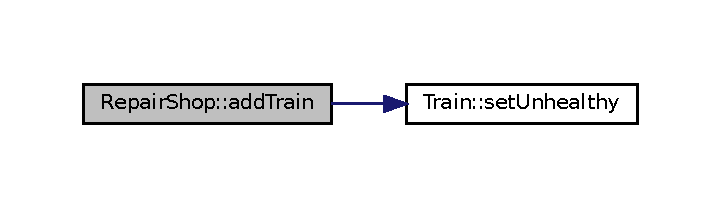
\includegraphics[width=346pt]{classRepairShop_a9232d4d4318014f7ca2665292f118938_cgraph}
\end{center}
\end{figure}
\mbox{\Hypertarget{classRepairShop_a1a5015fd8f8ad162254ef037ce15db48}\label{classRepairShop_a1a5015fd8f8ad162254ef037ce15db48}} 
\index{Repair\+Shop@{Repair\+Shop}!advance\+Day@{advance\+Day}}
\index{advance\+Day@{advance\+Day}!Repair\+Shop@{Repair\+Shop}}
\subsubsection{\texorpdfstring{advance\+Day()}{advanceDay()}}
{\footnotesize\ttfamily void Repair\+Shop\+::advance\+Day (\begin{DoxyParamCaption}{ }\end{DoxyParamCaption})}

Decrement days\+To\+Availability. If it becomes 0 after decrementation puts next train in currently being repaired. Here is the call graph for this function\+:
\nopagebreak
\begin{figure}[H]
\begin{center}
\leavevmode
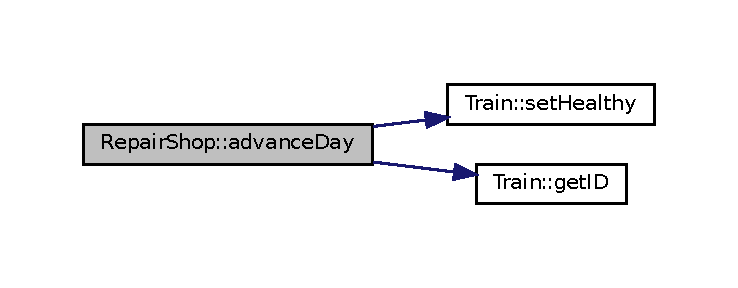
\includegraphics[width=350pt]{classRepairShop_a1a5015fd8f8ad162254ef037ce15db48_cgraph}
\end{center}
\end{figure}
\mbox{\Hypertarget{classRepairShop_ae0def7ba65f30ff9e7ddc0228c5b7ef8}\label{classRepairShop_ae0def7ba65f30ff9e7ddc0228c5b7ef8}} 
\index{Repair\+Shop@{Repair\+Shop}!get\+Days\+To\+Availability@{get\+Days\+To\+Availability}}
\index{get\+Days\+To\+Availability@{get\+Days\+To\+Availability}!Repair\+Shop@{Repair\+Shop}}
\subsubsection{\texorpdfstring{get\+Days\+To\+Availability()}{getDaysToAvailability()}}
{\footnotesize\ttfamily int Repair\+Shop\+::get\+Days\+To\+Availability (\begin{DoxyParamCaption}{ }\end{DoxyParamCaption}) const}

Get days left to start repairing next train.

\begin{DoxyReturn}{Returns}

\end{DoxyReturn}
\mbox{\Hypertarget{classRepairShop_a78f871f65f7bf4b0f068b9406998f351}\label{classRepairShop_a78f871f65f7bf4b0f068b9406998f351}} 
\index{Repair\+Shop@{Repair\+Shop}!get\+ID@{get\+ID}}
\index{get\+ID@{get\+ID}!Repair\+Shop@{Repair\+Shop}}
\subsubsection{\texorpdfstring{get\+I\+D()}{getID()}}
{\footnotesize\ttfamily \mbox{\hyperlink{project__utils_8h_a8f3a969054ad2200720b96e7e23dd4e1}{id\+\_\+t}} Repair\+Shop\+::get\+ID (\begin{DoxyParamCaption}{ }\end{DoxyParamCaption}) const}

Get the repair shop ID. \begin{DoxyReturn}{Returns}

\end{DoxyReturn}
\mbox{\Hypertarget{classRepairShop_ae470c339746dcb9ba5bb4c58195e0400}\label{classRepairShop_ae470c339746dcb9ba5bb4c58195e0400}} 
\index{Repair\+Shop@{Repair\+Shop}!get\+Name@{get\+Name}}
\index{get\+Name@{get\+Name}!Repair\+Shop@{Repair\+Shop}}
\subsubsection{\texorpdfstring{get\+Name()}{getName()}}
{\footnotesize\ttfamily const string \& Repair\+Shop\+::get\+Name (\begin{DoxyParamCaption}{ }\end{DoxyParamCaption}) const}

Get the name of the repair shop.

\begin{DoxyReturn}{Returns}

\end{DoxyReturn}
\mbox{\Hypertarget{classRepairShop_a5a1fe514136f22f66e8676421525c896}\label{classRepairShop_a5a1fe514136f22f66e8676421525c896}} 
\index{Repair\+Shop@{Repair\+Shop}!get\+X\+Coord@{get\+X\+Coord}}
\index{get\+X\+Coord@{get\+X\+Coord}!Repair\+Shop@{Repair\+Shop}}
\subsubsection{\texorpdfstring{get\+X\+Coord()}{getXCoord()}}
{\footnotesize\ttfamily int Repair\+Shop\+::get\+X\+Coord (\begin{DoxyParamCaption}{ }\end{DoxyParamCaption}) const}

Get the x coordinate of the repair shop.

\begin{DoxyReturn}{Returns}

\end{DoxyReturn}
\mbox{\Hypertarget{classRepairShop_a9c3c6369451f7da751ca1c6845d5d8f7}\label{classRepairShop_a9c3c6369451f7da751ca1c6845d5d8f7}} 
\index{Repair\+Shop@{Repair\+Shop}!get\+Y\+Coord@{get\+Y\+Coord}}
\index{get\+Y\+Coord@{get\+Y\+Coord}!Repair\+Shop@{Repair\+Shop}}
\subsubsection{\texorpdfstring{get\+Y\+Coord()}{getYCoord()}}
{\footnotesize\ttfamily int Repair\+Shop\+::get\+Y\+Coord (\begin{DoxyParamCaption}{ }\end{DoxyParamCaption}) const}

Get the y coordinate of the repair shop.

\begin{DoxyReturn}{Returns}

\end{DoxyReturn}
\mbox{\Hypertarget{classRepairShop_a7da5258b6595d1efc533b1eb8ec41ce3}\label{classRepairShop_a7da5258b6595d1efc533b1eb8ec41ce3}} 
\index{Repair\+Shop@{Repair\+Shop}!print\+Row@{print\+Row}}
\index{print\+Row@{print\+Row}!Repair\+Shop@{Repair\+Shop}}
\subsubsection{\texorpdfstring{print\+Row()}{printRow()}}
{\footnotesize\ttfamily void Repair\+Shop\+::print\+Row (\begin{DoxyParamCaption}\item[{std\+::ostream \&}]{os }\end{DoxyParamCaption})}

Print information in a fromatted line.


\begin{DoxyParams}{Parameters}
{\em os} & \\
\hline
\end{DoxyParams}
\mbox{\Hypertarget{classRepairShop_adb1e3f82716bac189d0f91ce9b9fd74e}\label{classRepairShop_adb1e3f82716bac189d0f91ce9b9fd74e}} 
\index{Repair\+Shop@{Repair\+Shop}!save@{save}}
\index{save@{save}!Repair\+Shop@{Repair\+Shop}}
\subsubsection{\texorpdfstring{save()}{save()}}
{\footnotesize\ttfamily void Repair\+Shop\+::save (\begin{DoxyParamCaption}\item[{std\+::ofstream \&}]{os }\end{DoxyParamCaption})}

Save information into file.


\begin{DoxyParams}{Parameters}
{\em os} & \\
\hline
\end{DoxyParams}
Here is the call graph for this function\+:
\nopagebreak
\begin{figure}[H]
\begin{center}
\leavevmode
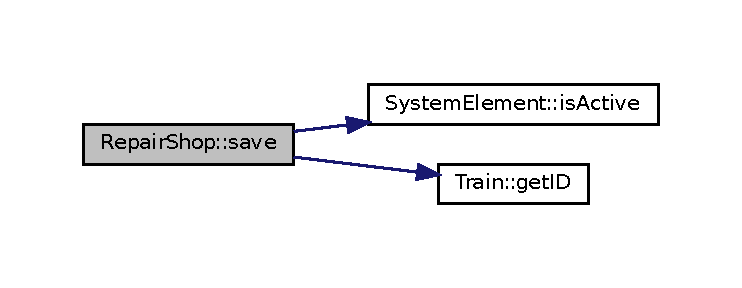
\includegraphics[width=350pt]{classRepairShop_adb1e3f82716bac189d0f91ce9b9fd74e_cgraph}
\end{center}
\end{figure}
\mbox{\Hypertarget{classRepairShop_af212410041d7bc7486e1eaa27864f527}\label{classRepairShop_af212410041d7bc7486e1eaa27864f527}} 
\index{Repair\+Shop@{Repair\+Shop}!set\+Days\+To\+Availability@{set\+Days\+To\+Availability}}
\index{set\+Days\+To\+Availability@{set\+Days\+To\+Availability}!Repair\+Shop@{Repair\+Shop}}
\subsubsection{\texorpdfstring{set\+Days\+To\+Availability()}{setDaysToAvailability()}}
{\footnotesize\ttfamily void Repair\+Shop\+::set\+Days\+To\+Availability (\begin{DoxyParamCaption}\item[{int}]{days\+To\+Availability }\end{DoxyParamCaption})}

Set the days\+To\+Availability variable.


\begin{DoxyParams}{Parameters}
{\em days\+To\+Availability} & \\
\hline
\end{DoxyParams}
\mbox{\Hypertarget{classRepairShop_ab3b24779f3d3bf3b9e9a70f1a4cb78c5}\label{classRepairShop_ab3b24779f3d3bf3b9e9a70f1a4cb78c5}} 
\index{Repair\+Shop@{Repair\+Shop}!set\+ID@{set\+ID}}
\index{set\+ID@{set\+ID}!Repair\+Shop@{Repair\+Shop}}
\subsubsection{\texorpdfstring{set\+I\+D()}{setID()}}
{\footnotesize\ttfamily void Repair\+Shop\+::set\+ID (\begin{DoxyParamCaption}\item[{\mbox{\hyperlink{project__utils_8h_a8f3a969054ad2200720b96e7e23dd4e1}{id\+\_\+t}}}]{id }\end{DoxyParamCaption})}

Set the repair shop ID. 

The documentation for this class was generated from the following files\+:\begin{DoxyCompactItemize}
\item 
system\+\_\+elements/\mbox{\hyperlink{RepairShop_8h}{Repair\+Shop.\+h}}\item 
system\+\_\+elements/\mbox{\hyperlink{RepairShop_8cpp}{Repair\+Shop.\+cpp}}\end{DoxyCompactItemize}

\hypertarget{structRepairShop_1_1RepairShopPQUtils}{}\section{Repair\+Shop\+:\+:Repair\+Shop\+P\+Q\+Utils Struct Reference}
\label{structRepairShop_1_1RepairShopPQUtils}\index{Repair\+Shop\+::\+Repair\+Shop\+P\+Q\+Utils@{Repair\+Shop\+::\+Repair\+Shop\+P\+Q\+Utils}}


{\ttfamily \#include $<$Repair\+Shop.\+h$>$}

\subsection*{Public Member Functions}
\begin{DoxyCompactItemize}
\item 
bool \mbox{\hyperlink{structRepairShop_1_1RepairShopPQUtils_ae278a2688d21efbd9ff519a72f8382e3}{operator()}} (const \mbox{\hyperlink{classRepairShop}{Repair\+Shop}} $\ast$rp1, const \mbox{\hyperlink{classRepairShop}{Repair\+Shop}} $\ast$rp2) const
\end{DoxyCompactItemize}


\subsection{Detailed Description}
Struct with function to be supplied to the Repair shops priority queue. 

\subsection{Member Function Documentation}
\mbox{\Hypertarget{structRepairShop_1_1RepairShopPQUtils_ae278a2688d21efbd9ff519a72f8382e3}\label{structRepairShop_1_1RepairShopPQUtils_ae278a2688d21efbd9ff519a72f8382e3}} 
\index{Repair\+Shop\+::\+Repair\+Shop\+P\+Q\+Utils@{Repair\+Shop\+::\+Repair\+Shop\+P\+Q\+Utils}!operator()@{operator()}}
\index{operator()@{operator()}!Repair\+Shop\+::\+Repair\+Shop\+P\+Q\+Utils@{Repair\+Shop\+::\+Repair\+Shop\+P\+Q\+Utils}}
\subsubsection{\texorpdfstring{operator()()}{operator()()}}
{\footnotesize\ttfamily bool Repair\+Shop\+::\+Repair\+Shop\+P\+Q\+Utils\+::operator() (\begin{DoxyParamCaption}\item[{const \mbox{\hyperlink{classRepairShop}{Repair\+Shop}} $\ast$}]{rp1,  }\item[{const \mbox{\hyperlink{classRepairShop}{Repair\+Shop}} $\ast$}]{rp2 }\end{DoxyParamCaption}) const\hspace{0.3cm}{\ttfamily [inline]}}

Comparison operator.


\begin{DoxyParams}{Parameters}
{\em rp1} & rhs \mbox{\hyperlink{classRepairShop}{Repair\+Shop}} \\
\hline
{\em rp2} & lhs \mbox{\hyperlink{classRepairShop}{Repair\+Shop}} \\
\hline
\end{DoxyParams}
\begin{DoxyReturn}{Returns}
bool 
\end{DoxyReturn}


The documentation for this struct was generated from the following file\+:\begin{DoxyCompactItemize}
\item 
system\+\_\+elements/\mbox{\hyperlink{RepairShop_8h}{Repair\+Shop.\+h}}\end{DoxyCompactItemize}

\hypertarget{classReverseDatesException}{}\section{Reverse\+Dates\+Exception Class Reference}
\label{classReverseDatesException}\index{Reverse\+Dates\+Exception@{Reverse\+Dates\+Exception}}


Exception reporting a trip\textquotesingle{}s arrival date happens before departure date.  




{\ttfamily \#include $<$Reverse\+Dates\+Exception.\+h$>$}



Inheritance diagram for Reverse\+Dates\+Exception\+:
\nopagebreak
\begin{figure}[H]
\begin{center}
\leavevmode
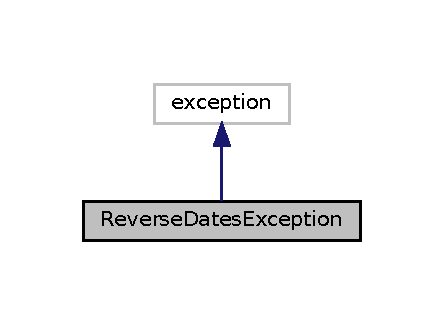
\includegraphics[width=213pt]{classReverseDatesException__inherit__graph}
\end{center}
\end{figure}


Collaboration diagram for Reverse\+Dates\+Exception\+:
\nopagebreak
\begin{figure}[H]
\begin{center}
\leavevmode
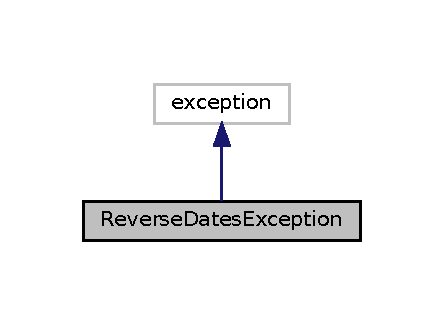
\includegraphics[width=213pt]{classReverseDatesException__coll__graph}
\end{center}
\end{figure}
\subsection*{Public Member Functions}
\begin{DoxyCompactItemize}
\item 
\mbox{\hyperlink{classReverseDatesException_afc245532384383f8f62b20358326c773}{Reverse\+Dates\+Exception}} (const std\+::string date1, const std\+::string date2)
\item 
const char $\ast$ \mbox{\hyperlink{classReverseDatesException_a52bb69fd0d940befffd9d69855ed6ae8}{what}} ()
\end{DoxyCompactItemize}


\subsection{Detailed Description}
Exception reporting a trip\textquotesingle{}s arrival date happens before departure date. 

\subsection{Constructor \& Destructor Documentation}
\mbox{\Hypertarget{classReverseDatesException_afc245532384383f8f62b20358326c773}\label{classReverseDatesException_afc245532384383f8f62b20358326c773}} 
\index{Reverse\+Dates\+Exception@{Reverse\+Dates\+Exception}!Reverse\+Dates\+Exception@{Reverse\+Dates\+Exception}}
\index{Reverse\+Dates\+Exception@{Reverse\+Dates\+Exception}!Reverse\+Dates\+Exception@{Reverse\+Dates\+Exception}}
\subsubsection{\texorpdfstring{Reverse\+Dates\+Exception()}{ReverseDatesException()}}
{\footnotesize\ttfamily Reverse\+Dates\+Exception\+::\+Reverse\+Dates\+Exception (\begin{DoxyParamCaption}\item[{const std\+::string}]{date1,  }\item[{const std\+::string}]{date2 }\end{DoxyParamCaption})}



\subsection{Member Function Documentation}
\mbox{\Hypertarget{classReverseDatesException_a52bb69fd0d940befffd9d69855ed6ae8}\label{classReverseDatesException_a52bb69fd0d940befffd9d69855ed6ae8}} 
\index{Reverse\+Dates\+Exception@{Reverse\+Dates\+Exception}!what@{what}}
\index{what@{what}!Reverse\+Dates\+Exception@{Reverse\+Dates\+Exception}}
\subsubsection{\texorpdfstring{what()}{what()}}
{\footnotesize\ttfamily const char $\ast$ Reverse\+Dates\+Exception\+::what (\begin{DoxyParamCaption}{ }\end{DoxyParamCaption})}



The documentation for this class was generated from the following files\+:\begin{DoxyCompactItemize}
\item 
exceptions/\mbox{\hyperlink{ReverseDatesException_8h}{Reverse\+Dates\+Exception.\+h}}\item 
exceptions/\mbox{\hyperlink{ReverseDatesException_8cpp}{Reverse\+Dates\+Exception.\+cpp}}\end{DoxyCompactItemize}

\hypertarget{classStation}{}\section{Station Class Reference}
\label{classStation}\index{Station@{Station}}


Class for representing a station in the system.  




{\ttfamily \#include $<$Station.\+h$>$}

\subsection*{Public Member Functions}
\begin{DoxyCompactItemize}
\item 
\mbox{\hyperlink{classStation_a53a471eb11c9431c3e89058d558f7601}{Station}} (std\+::string name)
\begin{DoxyCompactList}\small\item\em Construct a new \mbox{\hyperlink{classStation}{Station}} object. \end{DoxyCompactList}\item 
id\+\_\+t \mbox{\hyperlink{classStation_acbc5832d77cbe29c9006212b9cc32a42}{get\+ID}} () const
\begin{DoxyCompactList}\small\item\em Get the station ID. \end{DoxyCompactList}\item 
std\+::string \mbox{\hyperlink{classStation_ac823ae175ec0e2baff462ed9612c7bae}{get\+Name}} () const
\begin{DoxyCompactList}\small\item\em Get the \mbox{\hyperlink{classStation}{Station}}\textquotesingle{}s name. \end{DoxyCompactList}\item 
void \mbox{\hyperlink{classStation_a66c028cdffd79bddd0704235b051ff4e}{print\+Row}} (std\+::ostream \&os)
\begin{DoxyCompactList}\small\item\em Output station information in a row fashion. \end{DoxyCompactList}\end{DoxyCompactItemize}
\subsection*{Friends}
\begin{DoxyCompactItemize}
\item 
std\+::ostream \& \mbox{\hyperlink{classStation_ae5ca3266f8eead5634eb5926438392da}{operator$<$$<$}} (std\+::ostream \&os, \mbox{\hyperlink{classStation}{Station}} \&st)
\begin{DoxyCompactList}\small\item\em Output \mbox{\hyperlink{classStation}{Station}} object in a user friendly fashion. \end{DoxyCompactList}\end{DoxyCompactItemize}


\subsection{Detailed Description}
Class for representing a station in the system. 

\subsection{Constructor \& Destructor Documentation}
\mbox{\Hypertarget{classStation_a53a471eb11c9431c3e89058d558f7601}\label{classStation_a53a471eb11c9431c3e89058d558f7601}} 
\index{Station@{Station}!Station@{Station}}
\index{Station@{Station}!Station@{Station}}
\subsubsection{\texorpdfstring{Station()}{Station()}}
{\footnotesize\ttfamily Station\+::\+Station (\begin{DoxyParamCaption}\item[{std\+::string}]{name }\end{DoxyParamCaption})}



Construct a new \mbox{\hyperlink{classStation}{Station}} object. 


\begin{DoxyParams}{Parameters}
{\em name} & Name of the station. \\
\hline
\end{DoxyParams}


\subsection{Member Function Documentation}
\mbox{\Hypertarget{classStation_acbc5832d77cbe29c9006212b9cc32a42}\label{classStation_acbc5832d77cbe29c9006212b9cc32a42}} 
\index{Station@{Station}!get\+ID@{get\+ID}}
\index{get\+ID@{get\+ID}!Station@{Station}}
\subsubsection{\texorpdfstring{get\+I\+D()}{getID()}}
{\footnotesize\ttfamily id\+\_\+t Station\+::get\+ID (\begin{DoxyParamCaption}{ }\end{DoxyParamCaption}) const}



Get the station ID. 

\begin{DoxyReturn}{Returns}
id\+\_\+t 
\end{DoxyReturn}
\mbox{\Hypertarget{classStation_ac823ae175ec0e2baff462ed9612c7bae}\label{classStation_ac823ae175ec0e2baff462ed9612c7bae}} 
\index{Station@{Station}!get\+Name@{get\+Name}}
\index{get\+Name@{get\+Name}!Station@{Station}}
\subsubsection{\texorpdfstring{get\+Name()}{getName()}}
{\footnotesize\ttfamily string Station\+::get\+Name (\begin{DoxyParamCaption}{ }\end{DoxyParamCaption}) const}



Get the \mbox{\hyperlink{classStation}{Station}}\textquotesingle{}s name. 

\begin{DoxyReturn}{Returns}
std\+::string \mbox{\hyperlink{classStation}{Station}}\textquotesingle{}s name 
\end{DoxyReturn}
\mbox{\Hypertarget{classStation_a66c028cdffd79bddd0704235b051ff4e}\label{classStation_a66c028cdffd79bddd0704235b051ff4e}} 
\index{Station@{Station}!print\+Row@{print\+Row}}
\index{print\+Row@{print\+Row}!Station@{Station}}
\subsubsection{\texorpdfstring{print\+Row()}{printRow()}}
{\footnotesize\ttfamily void Station\+::print\+Row (\begin{DoxyParamCaption}\item[{std\+::ostream \&}]{os }\end{DoxyParamCaption})}



Output station information in a row fashion. 

Outputs the object\textquotesingle{}s information as it was a row in a table. Useful for outputing all \mbox{\hyperlink{classStation}{Station}} objects in the system.


\begin{DoxyParams}{Parameters}
{\em os} & The output stream to which the station will be output. \\
\hline
\end{DoxyParams}


\subsection{Friends And Related Function Documentation}
\mbox{\Hypertarget{classStation_ae5ca3266f8eead5634eb5926438392da}\label{classStation_ae5ca3266f8eead5634eb5926438392da}} 
\index{Station@{Station}!operator$<$$<$@{operator$<$$<$}}
\index{operator$<$$<$@{operator$<$$<$}!Station@{Station}}
\subsubsection{\texorpdfstring{operator$<$$<$}{operator<<}}
{\footnotesize\ttfamily std\+::ostream\& operator$<$$<$ (\begin{DoxyParamCaption}\item[{std\+::ostream \&}]{os,  }\item[{\mbox{\hyperlink{classStation}{Station}} \&}]{st }\end{DoxyParamCaption})\hspace{0.3cm}{\ttfamily [friend]}}



Output \mbox{\hyperlink{classStation}{Station}} object in a user friendly fashion. 


\begin{DoxyParams}{Parameters}
{\em os} & Output stream to wich \mbox{\hyperlink{classStation}{Station}} object will be output \\
\hline
{\em p} & \mbox{\hyperlink{classStation}{Station}} object to be output \\
\hline
\end{DoxyParams}
\begin{DoxyReturn}{Returns}
std\+::ostream\& 
\end{DoxyReturn}


The documentation for this class was generated from the following files\+:\begin{DoxyCompactItemize}
\item 
Station.\+h\item 
Station.\+cpp\end{DoxyCompactItemize}

\hypertarget{classSystem}{}\section{System Class Reference}
\label{classSystem}\index{System@{System}}
\subsection*{Public Member Functions}
\begin{DoxyCompactItemize}
\item 
\mbox{\Hypertarget{classSystem_aa4879a70a434d3b879090500b282de0b}\label{classSystem_aa4879a70a434d3b879090500b282de0b}} 
std\+::vector$<$ \mbox{\hyperlink{classPassenger}{Passenger}} $\ast$ $>$ \& {\bfseries get\+Passengers} ()
\item 
\mbox{\Hypertarget{classSystem_a97b3ac8c8d84fecbdd2c49df5e4b51bf}\label{classSystem_a97b3ac8c8d84fecbdd2c49df5e4b51bf}} 
std\+::vector$<$ \mbox{\hyperlink{classTrip}{Trip}} $\ast$ $>$ \& {\bfseries get\+Trips} ()
\item 
\mbox{\Hypertarget{classSystem_a44ee205bcb6c27bb1a7bc7fb545aef44}\label{classSystem_a44ee205bcb6c27bb1a7bc7fb545aef44}} 
std\+::vector$<$ \mbox{\hyperlink{classTrain}{Train}} $\ast$ $>$ \& {\bfseries get\+Trains} ()
\item 
\mbox{\Hypertarget{classSystem_a6f27512fba42cc093efd34fe10bf0045}\label{classSystem_a6f27512fba42cc093efd34fe10bf0045}} 
std\+::vector$<$ \mbox{\hyperlink{classStation}{Station}} $\ast$ $>$ \& {\bfseries get\+Stations} ()
\item 
\mbox{\Hypertarget{classSystem_a5a0348802d5cdb666f330b1e10d32727}\label{classSystem_a5a0348802d5cdb666f330b1e10d32727}} 
\mbox{\hyperlink{classPassenger}{Passenger}} $\ast$ {\bfseries get\+Passenger} (const id\+\_\+t id)
\item 
\mbox{\Hypertarget{classSystem_a518ff04299c8b37d3cbec814ac0b7ec6}\label{classSystem_a518ff04299c8b37d3cbec814ac0b7ec6}} 
\mbox{\hyperlink{classTrip}{Trip}} $\ast$ {\bfseries get\+Trip} (const id\+\_\+t id)
\item 
\mbox{\Hypertarget{classSystem_ac29b91a9dca7dd1bb4c39769a75d444f}\label{classSystem_ac29b91a9dca7dd1bb4c39769a75d444f}} 
\mbox{\hyperlink{classTrain}{Train}} $\ast$ {\bfseries get\+Train} (const id\+\_\+t id)
\item 
\mbox{\Hypertarget{classSystem_aaadc55451a0d43b7ba98ff5377de8e02}\label{classSystem_aaadc55451a0d43b7ba98ff5377de8e02}} 
\mbox{\hyperlink{classStation}{Station}} $\ast$ {\bfseries get\+Station} (const id\+\_\+t id)
\item 
\mbox{\Hypertarget{classSystem_a231710db7f31b3fec68f90fd90b292eb}\label{classSystem_a231710db7f31b3fec68f90fd90b292eb}} 
int {\bfseries get\+Station\+Index} (id\+\_\+t station\+ID)
\item 
\mbox{\Hypertarget{classSystem_a15d033a2efda45b83bbe0800698ae712}\label{classSystem_a15d033a2efda45b83bbe0800698ae712}} 
int {\bfseries get\+Train\+Index} (id\+\_\+t train\+ID)
\item 
\mbox{\Hypertarget{classSystem_aa431fdc152458fc39efb9a60e9f62f01}\label{classSystem_aa431fdc152458fc39efb9a60e9f62f01}} 
int {\bfseries get\+Trip\+Index} (id\+\_\+t trip\+ID)
\item 
\mbox{\Hypertarget{classSystem_a293b247432ab577c9bf0ba7285a6eeda}\label{classSystem_a293b247432ab577c9bf0ba7285a6eeda}} 
std\+::vector$<$ \mbox{\hyperlink{classTrip}{Trip}} $\ast$ $>$ {\bfseries search\+Trips} (\mbox{\hyperlink{classStation}{Station}} $\ast$src, \mbox{\hyperlink{classStation}{Station}} $\ast$dest, bool search\+By\+Arrival\+Date, \mbox{\hyperlink{classDate}{Date}} arrival\+Date)
\item 
\mbox{\Hypertarget{classSystem_a933891c246bf870518f334ea5666b95c}\label{classSystem_a933891c246bf870518f334ea5666b95c}} 
bool {\bfseries add\+Passenger} (\mbox{\hyperlink{classPassenger}{Passenger}} $\ast$passenger)
\item 
\mbox{\Hypertarget{classSystem_ad019d3f8d30be9b2f57842512f0393ed}\label{classSystem_ad019d3f8d30be9b2f57842512f0393ed}} 
bool {\bfseries add\+Trip} (\mbox{\hyperlink{classTrip}{Trip}} $\ast$trip)
\item 
\mbox{\Hypertarget{classSystem_a8022adc1c1f212c138ca9da7995bb422}\label{classSystem_a8022adc1c1f212c138ca9da7995bb422}} 
bool {\bfseries add\+Train} (\mbox{\hyperlink{classTrain}{Train}} $\ast$train)
\item 
\mbox{\Hypertarget{classSystem_abc5bda005d56392c66914ddd4f96e725}\label{classSystem_abc5bda005d56392c66914ddd4f96e725}} 
bool {\bfseries add\+Station} (\mbox{\hyperlink{classStation}{Station}} $\ast$station)
\item 
\mbox{\Hypertarget{classSystem_af31acdda711986978533367ce3a64276}\label{classSystem_af31acdda711986978533367ce3a64276}} 
bool {\bfseries remove\+Passenger} (id\+\_\+t id)
\item 
\mbox{\Hypertarget{classSystem_ae802cde42ae56b50adc02c76920e9001}\label{classSystem_ae802cde42ae56b50adc02c76920e9001}} 
bool {\bfseries remove\+Trip} (id\+\_\+t id)
\item 
\mbox{\Hypertarget{classSystem_ae582dd1c79cbd879ba1fbec5ceaab2fb}\label{classSystem_ae582dd1c79cbd879ba1fbec5ceaab2fb}} 
bool {\bfseries remove\+Station} (id\+\_\+t id)
\item 
\mbox{\Hypertarget{classSystem_acf1d845cdb88b43143b3f738214e866b}\label{classSystem_acf1d845cdb88b43143b3f738214e866b}} 
bool {\bfseries remove\+Train} (id\+\_\+t id)
\item 
\mbox{\Hypertarget{classSystem_a623d7369872a9af9b69b24bd2a3c71b1}\label{classSystem_a623d7369872a9af9b69b24bd2a3c71b1}} 
void {\bfseries create\+Passenger} (std\+::string name, \mbox{\hyperlink{classDate}{Date}} birth\+Date)
\item 
\mbox{\Hypertarget{classSystem_a9e317da5b607c6dee850089f340dd9e7}\label{classSystem_a9e317da5b607c6dee850089f340dd9e7}} 
void {\bfseries create\+Card} (\mbox{\hyperlink{classPassenger}{Passenger}} $\ast$p, std\+::string type)
\item 
\mbox{\Hypertarget{classSystem_ab8cf1529f497af79b72fe6cc59b08d60}\label{classSystem_ab8cf1529f497af79b72fe6cc59b08d60}} 
void {\bfseries create\+Station} (std\+::string name)
\item 
\mbox{\Hypertarget{classSystem_aa4cf09119e31e5bdf9d9187a7a60cd1a}\label{classSystem_aa4cf09119e31e5bdf9d9187a7a60cd1a}} 
void {\bfseries create\+Train} (uint max\+Seats)
\item 
\mbox{\Hypertarget{classSystem_aea8519bf009400085f8e499891b7eb37}\label{classSystem_aea8519bf009400085f8e499891b7eb37}} 
void {\bfseries create\+Trip} (uint base\+Price, \mbox{\hyperlink{classStation}{Station}} $\ast$source, \mbox{\hyperlink{classStation}{Station}} $\ast$destination, \mbox{\hyperlink{classTrain}{Train}} $\ast$train, const \mbox{\hyperlink{classDate}{Date}} daparture\+Date, const \mbox{\hyperlink{classDate}{Date}} arrival\+Date)
\item 
\mbox{\Hypertarget{classSystem_a360f9d625dbc649d567249642c1db53c}\label{classSystem_a360f9d625dbc649d567249642c1db53c}} 
void {\bfseries sort\+Passengers} ()
\item 
\mbox{\Hypertarget{classSystem_ae3b7301dda5863379777c863df0b976e}\label{classSystem_ae3b7301dda5863379777c863df0b976e}} 
void {\bfseries sort\+Passengers\+By\+Name} ()
\item 
\mbox{\Hypertarget{classSystem_a94f061c2fa79b7f0e4f175fc68a59246}\label{classSystem_a94f061c2fa79b7f0e4f175fc68a59246}} 
void {\bfseries sort\+Stations} ()
\item 
\mbox{\Hypertarget{classSystem_a3961bbb1e8a309ef37c4366731bbb813}\label{classSystem_a3961bbb1e8a309ef37c4366731bbb813}} 
void {\bfseries sort\+Trains} ()
\item 
\mbox{\Hypertarget{classSystem_a9122a0e24a88b5111959fdc87b23bc6b}\label{classSystem_a9122a0e24a88b5111959fdc87b23bc6b}} 
void {\bfseries sort\+Trips} ()
\item 
\mbox{\Hypertarget{classSystem_a3a2aace3c50cfbf7f9d2354cd858a59b}\label{classSystem_a3a2aace3c50cfbf7f9d2354cd858a59b}} 
void {\bfseries sort\+Trips\+By\+Date} ()
\item 
\mbox{\Hypertarget{classSystem_ac2b6f3d934b64f4fa56ffb1db1d261df}\label{classSystem_ac2b6f3d934b64f4fa56ffb1db1d261df}} 
bool {\bfseries process\+Ticket\+Purchase\+Request} (\mbox{\hyperlink{classTicketPurchaseRequest}{Ticket\+Purchase\+Request}} \&request)
\item 
\mbox{\Hypertarget{classSystem_aebffe11376f68cb17175f30ea517c10b}\label{classSystem_aebffe11376f68cb17175f30ea517c10b}} 
void {\bfseries process\+Cards} ()
\item 
\mbox{\Hypertarget{classSystem_ae5df9c6b2309272f8642cb16dbe5132e}\label{classSystem_ae5df9c6b2309272f8642cb16dbe5132e}} 
bool {\bfseries pay\+Card} (id\+\_\+t passenger\+ID)
\item 
\mbox{\Hypertarget{classSystem_a23c0b01d0e84fa4665ce85203ce6747b}\label{classSystem_a23c0b01d0e84fa4665ce85203ce6747b}} 
void {\bfseries list\+Passengers} (std\+::ostream \&os)
\item 
\mbox{\Hypertarget{classSystem_a06041827a7b47ad06eee9d121e42590c}\label{classSystem_a06041827a7b47ad06eee9d121e42590c}} 
void {\bfseries list\+Stations} (std\+::ostream \&os)
\item 
\mbox{\Hypertarget{classSystem_a0a6c0d8d1061893151f9b4ee3332ce85}\label{classSystem_a0a6c0d8d1061893151f9b4ee3332ce85}} 
void {\bfseries list\+Trains} (std\+::ostream \&os)
\item 
\mbox{\Hypertarget{classSystem_af11f201f6417c2658f35238d98c6f032}\label{classSystem_af11f201f6417c2658f35238d98c6f032}} 
void {\bfseries list\+Trips} (std\+::ostream \&os)
\item 
\mbox{\Hypertarget{classSystem_a1c5753d5c70d15dc3fe56fd5e421ba76}\label{classSystem_a1c5753d5c70d15dc3fe56fd5e421ba76}} 
void {\bfseries print\+Passengers} (std\+::ostream \&os) const
\item 
\mbox{\Hypertarget{classSystem_ac4b65c4fe2628e7d35b1027161e9d1da}\label{classSystem_ac4b65c4fe2628e7d35b1027161e9d1da}} 
void {\bfseries print\+Stations} (std\+::ostream \&os) const
\item 
\mbox{\Hypertarget{classSystem_af4610f38d80e01a18f2083a7c5fbd5ce}\label{classSystem_af4610f38d80e01a18f2083a7c5fbd5ce}} 
void {\bfseries print\+Trains} (std\+::ostream \&os) const
\item 
\mbox{\Hypertarget{classSystem_abaa61b6377abcfc61da32092e5d734d9}\label{classSystem_abaa61b6377abcfc61da32092e5d734d9}} 
void {\bfseries print\+Trips} (std\+::ostream \&os) const
\item 
\mbox{\Hypertarget{classSystem_aaad47fd0e1bf746a0bed32feb9553e53}\label{classSystem_aaad47fd0e1bf746a0bed32feb9553e53}} 
void {\bfseries print\+Sales} (std\+::ostream \&os) const
\end{DoxyCompactItemize}
\subsection*{Static Public Attributes}
\begin{DoxyCompactItemize}
\item 
\mbox{\Hypertarget{classSystem_a40d348884d1b737ecd26b4bc6509bf48}\label{classSystem_a40d348884d1b737ecd26b4bc6509bf48}} 
static \mbox{\hyperlink{classSystem}{System}} {\bfseries instance} = \mbox{\hyperlink{classSystem}{System}}()
\end{DoxyCompactItemize}
\subsection*{Friends}
\begin{DoxyCompactItemize}
\item 
\mbox{\Hypertarget{classSystem_a1efa95132e95a7a6b11c3b54916d66ae}\label{classSystem_a1efa95132e95a7a6b11c3b54916d66ae}} 
std\+::ostream \& {\bfseries operator$<$$<$} (std\+::ostream \&os, \mbox{\hyperlink{classSystem}{System}} \&sys)
\end{DoxyCompactItemize}


The documentation for this class was generated from the following files\+:\begin{DoxyCompactItemize}
\item 
System.\+h\item 
System.\+cpp\end{DoxyCompactItemize}

\hypertarget{classSystemElement}{}\section{System\+Element Class Reference}
\label{classSystemElement}\index{System\+Element@{System\+Element}}


{\ttfamily \#include $<$System\+Element.\+h$>$}



Inheritance diagram for System\+Element\+:
\nopagebreak
\begin{figure}[H]
\begin{center}
\leavevmode
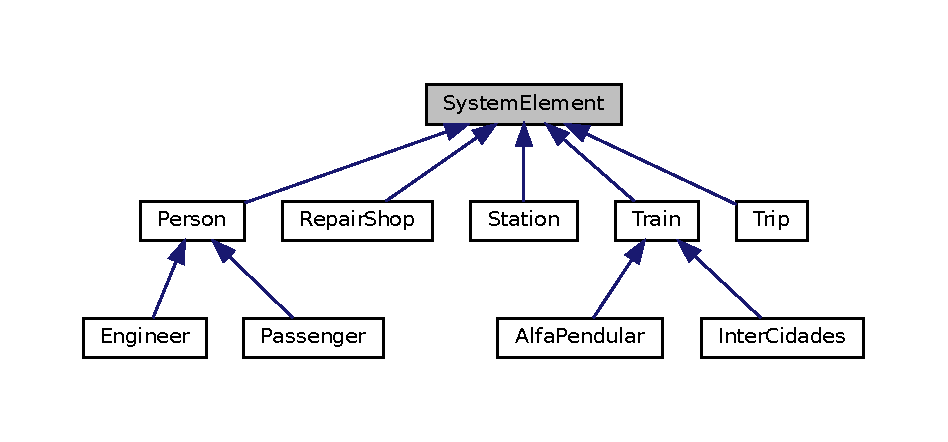
\includegraphics[width=350pt]{classSystemElement__inherit__graph}
\end{center}
\end{figure}
\subsection*{Public Member Functions}
\begin{DoxyCompactItemize}
\item 
\mbox{\hyperlink{classSystemElement_a212b0b8d05fc08ae3358cbae576e3f39}{System\+Element}} ()
\item 
void \mbox{\hyperlink{classSystemElement_a020e7af72158df06021525b5bb878e92}{set\+Active}} ()
\item 
void \mbox{\hyperlink{classSystemElement_aaa601d0e2960dd62d68e0f025f5eb362}{set\+Inactive}} ()
\item 
bool \mbox{\hyperlink{classSystemElement_a50987a52734db127a8ff3574903182d0}{is\+Active}} () const
\end{DoxyCompactItemize}


\subsection{Detailed Description}
A system element to be listed. 

\subsection{Constructor \& Destructor Documentation}
\mbox{\Hypertarget{classSystemElement_a212b0b8d05fc08ae3358cbae576e3f39}\label{classSystemElement_a212b0b8d05fc08ae3358cbae576e3f39}} 
\index{System\+Element@{System\+Element}!System\+Element@{System\+Element}}
\index{System\+Element@{System\+Element}!System\+Element@{System\+Element}}
\subsubsection{\texorpdfstring{System\+Element()}{SystemElement()}}
{\footnotesize\ttfamily System\+Element\+::\+System\+Element (\begin{DoxyParamCaption}{ }\end{DoxyParamCaption})}

Create a new \mbox{\hyperlink{classSystemElement}{System\+Element}} object. 

\subsection{Member Function Documentation}
\mbox{\Hypertarget{classSystemElement_a50987a52734db127a8ff3574903182d0}\label{classSystemElement_a50987a52734db127a8ff3574903182d0}} 
\index{System\+Element@{System\+Element}!is\+Active@{is\+Active}}
\index{is\+Active@{is\+Active}!System\+Element@{System\+Element}}
\subsubsection{\texorpdfstring{is\+Active()}{isActive()}}
{\footnotesize\ttfamily bool System\+Element\+::is\+Active (\begin{DoxyParamCaption}{ }\end{DoxyParamCaption}) const}

Tells if the element is active. \mbox{\Hypertarget{classSystemElement_a020e7af72158df06021525b5bb878e92}\label{classSystemElement_a020e7af72158df06021525b5bb878e92}} 
\index{System\+Element@{System\+Element}!set\+Active@{set\+Active}}
\index{set\+Active@{set\+Active}!System\+Element@{System\+Element}}
\subsubsection{\texorpdfstring{set\+Active()}{setActive()}}
{\footnotesize\ttfamily void System\+Element\+::set\+Active (\begin{DoxyParamCaption}{ }\end{DoxyParamCaption})}

Make the element active. \mbox{\Hypertarget{classSystemElement_aaa601d0e2960dd62d68e0f025f5eb362}\label{classSystemElement_aaa601d0e2960dd62d68e0f025f5eb362}} 
\index{System\+Element@{System\+Element}!set\+Inactive@{set\+Inactive}}
\index{set\+Inactive@{set\+Inactive}!System\+Element@{System\+Element}}
\subsubsection{\texorpdfstring{set\+Inactive()}{setInactive()}}
{\footnotesize\ttfamily void System\+Element\+::set\+Inactive (\begin{DoxyParamCaption}{ }\end{DoxyParamCaption})}

Make the element incative. 

The documentation for this class was generated from the following files\+:\begin{DoxyCompactItemize}
\item 
system\+\_\+elements/\mbox{\hyperlink{SystemElement_8h}{System\+Element.\+h}}\item 
system\+\_\+elements/\mbox{\hyperlink{SystemElement_8cpp}{System\+Element.\+cpp}}\end{DoxyCompactItemize}

\hypertarget{classTicketInvoice}{}\section{Ticket\+Invoice Class Reference}
\label{classTicketInvoice}\index{Ticket\+Invoice@{Ticket\+Invoice}}


Class for representing an invoice of a ticket purchase in the system.  




{\ttfamily \#include $<$Ticket\+Invoice.\+h$>$}

\subsection*{Public Member Functions}
\begin{DoxyCompactItemize}
\item 
\mbox{\hyperlink{classTicketInvoice_a38b37e5168ce71bbf37aceef8a6f6267}{Ticket\+Invoice}} (\mbox{\hyperlink{classPassenger}{Passenger}} $\ast$p, \mbox{\hyperlink{classTrip}{Trip}} $\ast$t)
\begin{DoxyCompactList}\small\item\em Construct a new Ticket Invoice object. \end{DoxyCompactList}\item 
const std\+::string \mbox{\hyperlink{classTicketInvoice_a9fdfdcd08ff90480ca85e027f57033e4}{get\+Passenger\+Name}} () const
\begin{DoxyCompactList}\small\item\em Get the \mbox{\hyperlink{classPassenger}{Passenger}} Name. \end{DoxyCompactList}\item 
const std\+::string \mbox{\hyperlink{classTicketInvoice_ad692197170d5cb11790dff71150ef891}{get\+Source\+Name}} () const
\begin{DoxyCompactList}\small\item\em Get the Source Name. \end{DoxyCompactList}\item 
const std\+::string \mbox{\hyperlink{classTicketInvoice_a1db4ffac81e11b765c6204278a3df8ff}{get\+Dest\+Name}} () const
\begin{DoxyCompactList}\small\item\em Get the Dest Name. \end{DoxyCompactList}\item 
const std\+::string \mbox{\hyperlink{classTicketInvoice_a97998091765f01ff9f394210530a89ed}{get\+Price\+String}} () const
\begin{DoxyCompactList}\small\item\em Get the Price String. \end{DoxyCompactList}\item 
const \mbox{\hyperlink{project__utils_8h_a91ad9478d81a7aaf2593e8d9c3d06a14}{uint}} \mbox{\hyperlink{classTicketInvoice_a3758bface685702a6229d617691663e1}{get\+Price}} () const
\begin{DoxyCompactList}\small\item\em Get the Price. \end{DoxyCompactList}\item 
void \mbox{\hyperlink{classTicketInvoice_afeed9962f0276861876a001e372d2063}{set\+Price}} (\mbox{\hyperlink{project__utils_8h_a91ad9478d81a7aaf2593e8d9c3d06a14}{uint}} price)
\begin{DoxyCompactList}\small\item\em Set the Price. \end{DoxyCompactList}\end{DoxyCompactItemize}
\subsection*{Friends}
\begin{DoxyCompactItemize}
\item 
std\+::ostream \& \mbox{\hyperlink{classTicketInvoice_ae78ba81ba79ed7e8c9e8cd23a910f00d}{operator$<$$<$}} (std\+::ostream \&os, \mbox{\hyperlink{classTicketInvoice}{Ticket\+Invoice}} \&in)
\end{DoxyCompactItemize}


\subsection{Detailed Description}
Class for representing an invoice of a ticket purchase in the system. 

\subsection{Constructor \& Destructor Documentation}
\mbox{\Hypertarget{classTicketInvoice_a38b37e5168ce71bbf37aceef8a6f6267}\label{classTicketInvoice_a38b37e5168ce71bbf37aceef8a6f6267}} 
\index{Ticket\+Invoice@{Ticket\+Invoice}!Ticket\+Invoice@{Ticket\+Invoice}}
\index{Ticket\+Invoice@{Ticket\+Invoice}!Ticket\+Invoice@{Ticket\+Invoice}}
\subsubsection{\texorpdfstring{Ticket\+Invoice()}{TicketInvoice()}}
{\footnotesize\ttfamily Ticket\+Invoice\+::\+Ticket\+Invoice (\begin{DoxyParamCaption}\item[{\mbox{\hyperlink{classPassenger}{Passenger}} $\ast$}]{p,  }\item[{\mbox{\hyperlink{classTrip}{Trip}} $\ast$}]{t }\end{DoxyParamCaption})}



Construct a new Ticket Invoice object. 


\begin{DoxyParams}{Parameters}
{\em p} & Pointer to the passanger that has done the purchase \\
\hline
{\em t} & \mbox{\hyperlink{classTrip}{Trip}} to which the ticket has been purchased \\
\hline
\end{DoxyParams}
Here is the call graph for this function\+:
\nopagebreak
\begin{figure}[H]
\begin{center}
\leavevmode
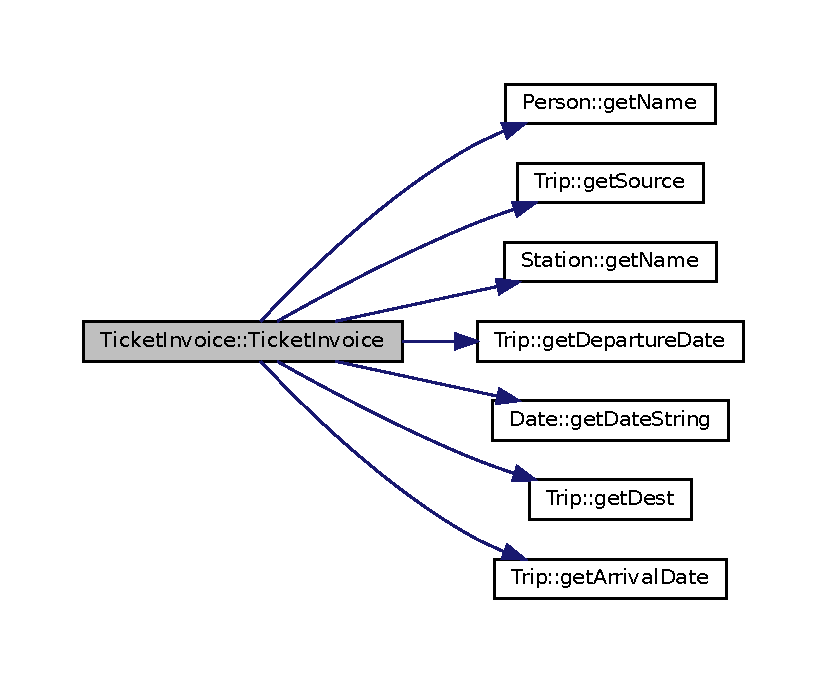
\includegraphics[width=350pt]{classTicketInvoice_a38b37e5168ce71bbf37aceef8a6f6267_cgraph}
\end{center}
\end{figure}


\subsection{Member Function Documentation}
\mbox{\Hypertarget{classTicketInvoice_a1db4ffac81e11b765c6204278a3df8ff}\label{classTicketInvoice_a1db4ffac81e11b765c6204278a3df8ff}} 
\index{Ticket\+Invoice@{Ticket\+Invoice}!get\+Dest\+Name@{get\+Dest\+Name}}
\index{get\+Dest\+Name@{get\+Dest\+Name}!Ticket\+Invoice@{Ticket\+Invoice}}
\subsubsection{\texorpdfstring{get\+Dest\+Name()}{getDestName()}}
{\footnotesize\ttfamily const string Ticket\+Invoice\+::get\+Dest\+Name (\begin{DoxyParamCaption}{ }\end{DoxyParamCaption}) const}



Get the Dest Name. 

\begin{DoxyReturn}{Returns}
const std\+::string Name of the destination station 
\end{DoxyReturn}
\mbox{\Hypertarget{classTicketInvoice_a9fdfdcd08ff90480ca85e027f57033e4}\label{classTicketInvoice_a9fdfdcd08ff90480ca85e027f57033e4}} 
\index{Ticket\+Invoice@{Ticket\+Invoice}!get\+Passenger\+Name@{get\+Passenger\+Name}}
\index{get\+Passenger\+Name@{get\+Passenger\+Name}!Ticket\+Invoice@{Ticket\+Invoice}}
\subsubsection{\texorpdfstring{get\+Passenger\+Name()}{getPassengerName()}}
{\footnotesize\ttfamily const string Ticket\+Invoice\+::get\+Passenger\+Name (\begin{DoxyParamCaption}{ }\end{DoxyParamCaption}) const}



Get the \mbox{\hyperlink{classPassenger}{Passenger}} Name. 

\begin{DoxyReturn}{Returns}
const std\+::string Name of the passenger 
\end{DoxyReturn}
\mbox{\Hypertarget{classTicketInvoice_a3758bface685702a6229d617691663e1}\label{classTicketInvoice_a3758bface685702a6229d617691663e1}} 
\index{Ticket\+Invoice@{Ticket\+Invoice}!get\+Price@{get\+Price}}
\index{get\+Price@{get\+Price}!Ticket\+Invoice@{Ticket\+Invoice}}
\subsubsection{\texorpdfstring{get\+Price()}{getPrice()}}
{\footnotesize\ttfamily const \mbox{\hyperlink{project__utils_8h_a91ad9478d81a7aaf2593e8d9c3d06a14}{uint}} Ticket\+Invoice\+::get\+Price (\begin{DoxyParamCaption}{ }\end{DoxyParamCaption}) const}



Get the Price. 

\begin{DoxyReturn}{Returns}
const uint The price in cents 
\end{DoxyReturn}
\mbox{\Hypertarget{classTicketInvoice_a97998091765f01ff9f394210530a89ed}\label{classTicketInvoice_a97998091765f01ff9f394210530a89ed}} 
\index{Ticket\+Invoice@{Ticket\+Invoice}!get\+Price\+String@{get\+Price\+String}}
\index{get\+Price\+String@{get\+Price\+String}!Ticket\+Invoice@{Ticket\+Invoice}}
\subsubsection{\texorpdfstring{get\+Price\+String()}{getPriceString()}}
{\footnotesize\ttfamily const string Ticket\+Invoice\+::get\+Price\+String (\begin{DoxyParamCaption}{ }\end{DoxyParamCaption}) const}



Get the Price String. 

\begin{DoxyReturn}{Returns}
const std\+::string A string representing the price in euros(not cents) 
\end{DoxyReturn}
\mbox{\Hypertarget{classTicketInvoice_ad692197170d5cb11790dff71150ef891}\label{classTicketInvoice_ad692197170d5cb11790dff71150ef891}} 
\index{Ticket\+Invoice@{Ticket\+Invoice}!get\+Source\+Name@{get\+Source\+Name}}
\index{get\+Source\+Name@{get\+Source\+Name}!Ticket\+Invoice@{Ticket\+Invoice}}
\subsubsection{\texorpdfstring{get\+Source\+Name()}{getSourceName()}}
{\footnotesize\ttfamily const string Ticket\+Invoice\+::get\+Source\+Name (\begin{DoxyParamCaption}{ }\end{DoxyParamCaption}) const}



Get the Source Name. 

\begin{DoxyReturn}{Returns}
const std\+::string Name of the source station 
\end{DoxyReturn}
\mbox{\Hypertarget{classTicketInvoice_afeed9962f0276861876a001e372d2063}\label{classTicketInvoice_afeed9962f0276861876a001e372d2063}} 
\index{Ticket\+Invoice@{Ticket\+Invoice}!set\+Price@{set\+Price}}
\index{set\+Price@{set\+Price}!Ticket\+Invoice@{Ticket\+Invoice}}
\subsubsection{\texorpdfstring{set\+Price()}{setPrice()}}
{\footnotesize\ttfamily void Ticket\+Invoice\+::set\+Price (\begin{DoxyParamCaption}\item[{\mbox{\hyperlink{project__utils_8h_a91ad9478d81a7aaf2593e8d9c3d06a14}{uint}}}]{price }\end{DoxyParamCaption})}



Set the Price. 


\begin{DoxyParams}{Parameters}
{\em price} & \\
\hline
\end{DoxyParams}


\subsection{Friends And Related Function Documentation}
\mbox{\Hypertarget{classTicketInvoice_ae78ba81ba79ed7e8c9e8cd23a910f00d}\label{classTicketInvoice_ae78ba81ba79ed7e8c9e8cd23a910f00d}} 
\index{Ticket\+Invoice@{Ticket\+Invoice}!operator$<$$<$@{operator$<$$<$}}
\index{operator$<$$<$@{operator$<$$<$}!Ticket\+Invoice@{Ticket\+Invoice}}
\subsubsection{\texorpdfstring{operator$<$$<$}{operator<<}}
{\footnotesize\ttfamily std\+::ostream\& operator$<$$<$ (\begin{DoxyParamCaption}\item[{std\+::ostream \&}]{os,  }\item[{\mbox{\hyperlink{classTicketInvoice}{Ticket\+Invoice}} \&}]{in }\end{DoxyParamCaption})\hspace{0.3cm}{\ttfamily [friend]}}



The documentation for this class was generated from the following files\+:\begin{DoxyCompactItemize}
\item 
\mbox{\hyperlink{TicketInvoice_8h}{Ticket\+Invoice.\+h}}\item 
\mbox{\hyperlink{TicketInvoice_8cpp}{Ticket\+Invoice.\+cpp}}\end{DoxyCompactItemize}

\hypertarget{classTicketPurchaseRequest}{}\section{Ticket\+Purchase\+Request Class Reference}
\label{classTicketPurchaseRequest}\index{Ticket\+Purchase\+Request@{Ticket\+Purchase\+Request}}
\subsection*{Public Member Functions}
\begin{DoxyCompactItemize}
\item 
\mbox{\Hypertarget{classTicketPurchaseRequest_aaa01be19b8a8ef88428f4d1dc3a3c63c}\label{classTicketPurchaseRequest_aaa01be19b8a8ef88428f4d1dc3a3c63c}} 
{\bfseries Ticket\+Purchase\+Request} (\mbox{\hyperlink{classPassenger}{Passenger}} $\ast$passenger, \mbox{\hyperlink{classTrip}{Trip}} $\ast$t)
\item 
\mbox{\Hypertarget{classTicketPurchaseRequest_a08428a7617aa26c16702420e61ce0312}\label{classTicketPurchaseRequest_a08428a7617aa26c16702420e61ce0312}} 
const \mbox{\hyperlink{classPassenger}{Passenger}} $\ast$ {\bfseries get\+Passenger} () const
\item 
\mbox{\Hypertarget{classTicketPurchaseRequest_a7ae48dcccbcddb298fae1bd74048570b}\label{classTicketPurchaseRequest_a7ae48dcccbcddb298fae1bd74048570b}} 
const \mbox{\hyperlink{classTrip}{Trip}} $\ast$ {\bfseries get\+Trip} () const
\item 
\mbox{\Hypertarget{classTicketPurchaseRequest_a289ba4fd54f5a0e5a8e8e4eecbff6b23}\label{classTicketPurchaseRequest_a289ba4fd54f5a0e5a8e8e4eecbff6b23}} 
void {\bfseries set\+Price} (uint price)
\item 
\mbox{\Hypertarget{classTicketPurchaseRequest_a626107dad44c79663d318573e5c6bae2}\label{classTicketPurchaseRequest_a626107dad44c79663d318573e5c6bae2}} 
void {\bfseries print\+Invoice} (std\+::ostream \&os)
\end{DoxyCompactItemize}
\subsection*{Friends}
\begin{DoxyCompactItemize}
\item 
\mbox{\Hypertarget{classTicketPurchaseRequest_af18a9ee98e70982bfe2975391d7221a5}\label{classTicketPurchaseRequest_af18a9ee98e70982bfe2975391d7221a5}} 
class {\bfseries System}
\end{DoxyCompactItemize}


The documentation for this class was generated from the following files\+:\begin{DoxyCompactItemize}
\item 
Ticket\+Purchase\+Request.\+h\item 
Ticket\+Purchase\+Request.\+cpp\end{DoxyCompactItemize}

\hypertarget{classTrain}{}\section{Train Class Reference}
\label{classTrain}\index{Train@{Train}}


Class for representing a train in the system.  




{\ttfamily \#include $<$Train.\+h$>$}

\subsection*{Public Member Functions}
\begin{DoxyCompactItemize}
\item 
\mbox{\hyperlink{classTrain_aa965be5e5d076d2743301c5d75ce4401}{Train}} (uint total\+Seats)
\begin{DoxyCompactList}\small\item\em Construct a new \mbox{\hyperlink{classTrain}{Train}} object. \end{DoxyCompactList}\item 
id\+\_\+t \mbox{\hyperlink{classTrain_a7310ae0bc5b43ea392e4fa62630ee56b}{get\+ID}} () const
\begin{DoxyCompactList}\small\item\em Get the train ID. \end{DoxyCompactList}\item 
uint \mbox{\hyperlink{classTrain_a93cd372664bac4ba28fa36e40316444a}{get\+Max\+Seats}} ()
\begin{DoxyCompactList}\small\item\em Get the max capacity. \end{DoxyCompactList}\item 
void \mbox{\hyperlink{classTrain_a3fd1c87c2152aa96cc6928f0aea37e21}{print\+Row}} (std\+::ostream \&os)
\begin{DoxyCompactList}\small\item\em Output train information in a row fashion. \end{DoxyCompactList}\end{DoxyCompactItemize}
\subsection*{Friends}
\begin{DoxyCompactItemize}
\item 
\mbox{\Hypertarget{classTrain_ab4c39558eb319a2f509b128f1fc90bd8}\label{classTrain_ab4c39558eb319a2f509b128f1fc90bd8}} 
std\+::ostream \& {\bfseries operator$<$$<$} (std\+::ostream \&os, \mbox{\hyperlink{classTrain}{Train}} \&tr)
\end{DoxyCompactItemize}


\subsection{Detailed Description}
Class for representing a train in the system. 

\subsection{Constructor \& Destructor Documentation}
\mbox{\Hypertarget{classTrain_aa965be5e5d076d2743301c5d75ce4401}\label{classTrain_aa965be5e5d076d2743301c5d75ce4401}} 
\index{Train@{Train}!Train@{Train}}
\index{Train@{Train}!Train@{Train}}
\subsubsection{\texorpdfstring{Train()}{Train()}}
{\footnotesize\ttfamily Train\+::\+Train (\begin{DoxyParamCaption}\item[{uint}]{total\+Seats }\end{DoxyParamCaption})}



Construct a new \mbox{\hyperlink{classTrain}{Train}} object. 


\begin{DoxyParams}{Parameters}
{\em total\+Seats} & Max capacity of train \\
\hline
\end{DoxyParams}


\subsection{Member Function Documentation}
\mbox{\Hypertarget{classTrain_a7310ae0bc5b43ea392e4fa62630ee56b}\label{classTrain_a7310ae0bc5b43ea392e4fa62630ee56b}} 
\index{Train@{Train}!get\+ID@{get\+ID}}
\index{get\+ID@{get\+ID}!Train@{Train}}
\subsubsection{\texorpdfstring{get\+I\+D()}{getID()}}
{\footnotesize\ttfamily id\+\_\+t Train\+::get\+ID (\begin{DoxyParamCaption}{ }\end{DoxyParamCaption}) const}



Get the train ID. 

\begin{DoxyReturn}{Returns}
id\+\_\+t 
\end{DoxyReturn}
\mbox{\Hypertarget{classTrain_a93cd372664bac4ba28fa36e40316444a}\label{classTrain_a93cd372664bac4ba28fa36e40316444a}} 
\index{Train@{Train}!get\+Max\+Seats@{get\+Max\+Seats}}
\index{get\+Max\+Seats@{get\+Max\+Seats}!Train@{Train}}
\subsubsection{\texorpdfstring{get\+Max\+Seats()}{getMaxSeats()}}
{\footnotesize\ttfamily uint Train\+::get\+Max\+Seats (\begin{DoxyParamCaption}{ }\end{DoxyParamCaption})}



Get the max capacity. 

\begin{DoxyReturn}{Returns}
uint 
\end{DoxyReturn}
\mbox{\Hypertarget{classTrain_a3fd1c87c2152aa96cc6928f0aea37e21}\label{classTrain_a3fd1c87c2152aa96cc6928f0aea37e21}} 
\index{Train@{Train}!print\+Row@{print\+Row}}
\index{print\+Row@{print\+Row}!Train@{Train}}
\subsubsection{\texorpdfstring{print\+Row()}{printRow()}}
{\footnotesize\ttfamily void Train\+::print\+Row (\begin{DoxyParamCaption}\item[{std\+::ostream \&}]{os }\end{DoxyParamCaption})}



Output train information in a row fashion. 

Outputs the object\textquotesingle{}s information as it was a row in a table. Useful for outputing all train objects in the system.


\begin{DoxyParams}{Parameters}
{\em os} & The output stream to which the train will be output. \\
\hline
\end{DoxyParams}


The documentation for this class was generated from the following files\+:\begin{DoxyCompactItemize}
\item 
Train.\+h\item 
Train.\+cpp\end{DoxyCompactItemize}

\hypertarget{classTrip}{}\section{Trip Class Reference}
\label{classTrip}\index{Trip@{Trip}}
\subsection*{Public Member Functions}
\begin{DoxyCompactItemize}
\item 
\mbox{\Hypertarget{classTrip_ad7244e90c71e27914dab013835883502}\label{classTrip_ad7244e90c71e27914dab013835883502}} 
{\bfseries Trip} (uint base\+Price, \mbox{\hyperlink{classStation}{Station}} $\ast$source, \mbox{\hyperlink{classStation}{Station}} $\ast$destination, \mbox{\hyperlink{classTrain}{Train}} $\ast$train, const std\+::string daparture\+Date, const std\+::string arrival\+Date)
\item 
\mbox{\Hypertarget{classTrip_a7770a61e1211789c80b003eeedcaa09c}\label{classTrip_a7770a61e1211789c80b003eeedcaa09c}} 
id\+\_\+t {\bfseries get\+ID} () const
\item 
\mbox{\Hypertarget{classTrip_aa356ea90590c617311c911c98aac4093}\label{classTrip_aa356ea90590c617311c911c98aac4093}} 
float {\bfseries get\+Base\+Price} () const
\item 
\mbox{\Hypertarget{classTrip_a65b45d4816c85d47ef743e7c1cfe807f}\label{classTrip_a65b45d4816c85d47ef743e7c1cfe807f}} 
\mbox{\hyperlink{classStation}{Station}} $\ast$ {\bfseries get\+Source} () const
\item 
\mbox{\Hypertarget{classTrip_a459ae85fc25404ba616fabfb4b4165f4}\label{classTrip_a459ae85fc25404ba616fabfb4b4165f4}} 
\mbox{\hyperlink{classStation}{Station}} $\ast$ {\bfseries get\+Dest} () const
\item 
\mbox{\Hypertarget{classTrip_a7595a39e9aa91e321d37b1696da50024}\label{classTrip_a7595a39e9aa91e321d37b1696da50024}} 
\mbox{\hyperlink{classTrain}{Train}} $\ast$ {\bfseries get\+Train} () const
\item 
\mbox{\Hypertarget{classTrip_ac506905deb66415b2fcee1c89579e628}\label{classTrip_ac506905deb66415b2fcee1c89579e628}} 
const \mbox{\hyperlink{classDate}{Date}} \& {\bfseries get\+Departure\+Date} () const
\item 
\mbox{\Hypertarget{classTrip_a6dddee29651df86b5a2c45bd2e1d2fc6}\label{classTrip_a6dddee29651df86b5a2c45bd2e1d2fc6}} 
const \mbox{\hyperlink{classDate}{Date}} \& {\bfseries get\+Arrival\+Date} () const
\item 
\mbox{\Hypertarget{classTrip_a00e2b65d40562051bfe4124f581a49e1}\label{classTrip_a00e2b65d40562051bfe4124f581a49e1}} 
bool {\bfseries book\+Seat} ()
\item 
\mbox{\Hypertarget{classTrip_a233bab5c803f51ee5e79c611a15699c0}\label{classTrip_a233bab5c803f51ee5e79c611a15699c0}} 
void {\bfseries print\+Row} (std\+::ostream \&os)
\end{DoxyCompactItemize}
\subsection*{Friends}
\begin{DoxyCompactItemize}
\item 
\mbox{\Hypertarget{classTrip_ad143ba29c1778aa25a53301503c3f2bd}\label{classTrip_ad143ba29c1778aa25a53301503c3f2bd}} 
std\+::ostream \& {\bfseries operator$<$$<$} (std\+::ostream \&os, \mbox{\hyperlink{classTrip}{Trip}} \&tr)
\end{DoxyCompactItemize}


The documentation for this class was generated from the following files\+:\begin{DoxyCompactItemize}
\item 
Trip.\+h\item 
Trip.\+cpp\end{DoxyCompactItemize}

\hypertarget{classTripPastException}{}\section{Trip\+Past\+Exception Class Reference}
\label{classTripPastException}\index{Trip\+Past\+Exception@{Trip\+Past\+Exception}}


An exception reporting that a trip is already in the past.  




{\ttfamily \#include $<$Trip\+Past\+Exception.\+h$>$}



Inheritance diagram for Trip\+Past\+Exception\+:
\nopagebreak
\begin{figure}[H]
\begin{center}
\leavevmode
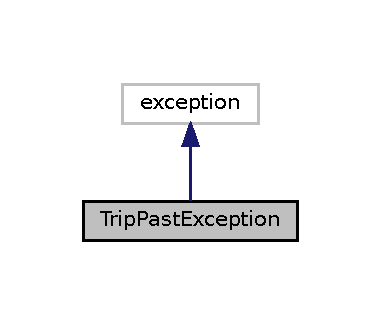
\includegraphics[width=183pt]{classTripPastException__inherit__graph}
\end{center}
\end{figure}


Collaboration diagram for Trip\+Past\+Exception\+:
\nopagebreak
\begin{figure}[H]
\begin{center}
\leavevmode
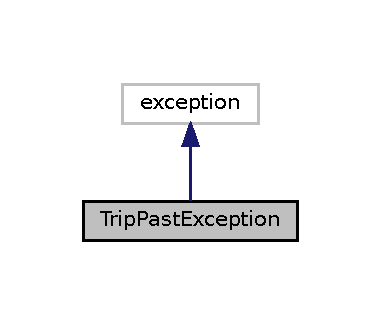
\includegraphics[width=183pt]{classTripPastException__coll__graph}
\end{center}
\end{figure}
\subsection*{Public Member Functions}
\begin{DoxyCompactItemize}
\item 
const char $\ast$ \mbox{\hyperlink{classTripPastException_a917f7042145fb1cbc2d43efb9f43f3f6}{what}} ()
\end{DoxyCompactItemize}


\subsection{Detailed Description}
An exception reporting that a trip is already in the past. 

\subsection{Member Function Documentation}
\mbox{\Hypertarget{classTripPastException_a917f7042145fb1cbc2d43efb9f43f3f6}\label{classTripPastException_a917f7042145fb1cbc2d43efb9f43f3f6}} 
\index{Trip\+Past\+Exception@{Trip\+Past\+Exception}!what@{what}}
\index{what@{what}!Trip\+Past\+Exception@{Trip\+Past\+Exception}}
\subsubsection{\texorpdfstring{what()}{what()}}
{\footnotesize\ttfamily const char $\ast$ Trip\+Past\+Exception\+::what (\begin{DoxyParamCaption}{ }\end{DoxyParamCaption})}



The documentation for this class was generated from the following files\+:\begin{DoxyCompactItemize}
\item 
exceptions/\mbox{\hyperlink{TripPastException_8h}{Trip\+Past\+Exception.\+h}}\item 
exceptions/\mbox{\hyperlink{TripPastException_8cpp}{Trip\+Past\+Exception.\+cpp}}\end{DoxyCompactItemize}

\chapter{File Documentation}
\hypertarget{Date_8cpp}{}\section{Date.\+cpp File Reference}
\label{Date_8cpp}\index{Date.\+cpp@{Date.\+cpp}}
{\ttfamily \#include \char`\"{}Date.\+h\char`\"{}}\newline
{\ttfamily \#include \char`\"{}exceptions/\+Invalid\+Date\+Exception.\+h\char`\"{}}\newline
{\ttfamily \#include $<$iomanip$>$}\newline
{\ttfamily \#include $<$sstream$>$}\newline
{\ttfamily \#include $<$algorithm$>$}\newline
Include dependency graph for Date.\+cpp\+:
\nopagebreak
\begin{figure}[H]
\begin{center}
\leavevmode
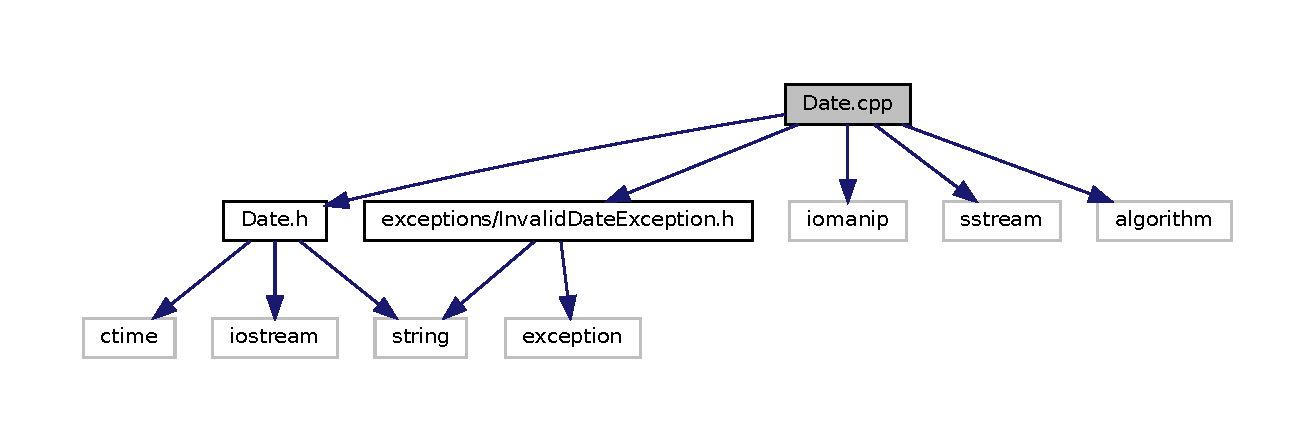
\includegraphics[width=350pt]{Date_8cpp__incl}
\end{center}
\end{figure}
\subsection*{Functions}
\begin{DoxyCompactItemize}
\item 
std\+::ostream \& \mbox{\hyperlink{Date_8cpp_a2f114c7aa1398dac0f21b888bcb40f3e}{operator$<$$<$}} (std\+::ostream \&o, \mbox{\hyperlink{classDate}{Date}} \&d)
\end{DoxyCompactItemize}


\subsection{Function Documentation}
\mbox{\Hypertarget{Date_8cpp_a2f114c7aa1398dac0f21b888bcb40f3e}\label{Date_8cpp_a2f114c7aa1398dac0f21b888bcb40f3e}} 
\index{Date.\+cpp@{Date.\+cpp}!operator$<$$<$@{operator$<$$<$}}
\index{operator$<$$<$@{operator$<$$<$}!Date.\+cpp@{Date.\+cpp}}
\subsubsection{\texorpdfstring{operator$<$$<$()}{operator<<()}}
{\footnotesize\ttfamily std\+::ostream\& operator$<$$<$ (\begin{DoxyParamCaption}\item[{std\+::ostream \&}]{o,  }\item[{\mbox{\hyperlink{classDate}{Date}} \&}]{d }\end{DoxyParamCaption})}

Passes a string of the date, to the output stream, in the following format\+: \char`\"{}dd-\/mm-\/yyyy H\+H\+:\+M\+M\char`\"{}


\begin{DoxyParams}{Parameters}
{\em o} & ouput stream \\
\hline
{\em d} & date object \\
\hline
\end{DoxyParams}
\begin{DoxyReturn}{Returns}
std\+::ostream\& reference to the output stream passed as argument 
\end{DoxyReturn}
Here is the call graph for this function\+:
\nopagebreak
\begin{figure}[H]
\begin{center}
\leavevmode
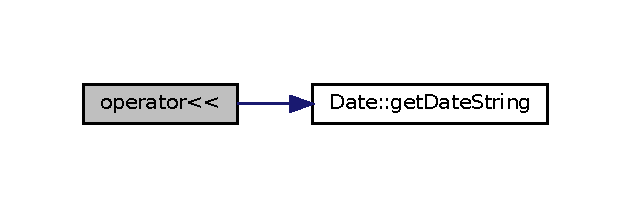
\includegraphics[width=303pt]{Date_8cpp_a2f114c7aa1398dac0f21b888bcb40f3e_cgraph}
\end{center}
\end{figure}

\hypertarget{Date_8h}{}\section{Date.\+h File Reference}
\label{Date_8h}\index{Date.\+h@{Date.\+h}}
{\ttfamily \#include $<$ctime$>$}\newline
{\ttfamily \#include $<$iostream$>$}\newline
{\ttfamily \#include $<$string$>$}\newline
Include dependency graph for Date.\+h\+:
\nopagebreak
\begin{figure}[H]
\begin{center}
\leavevmode
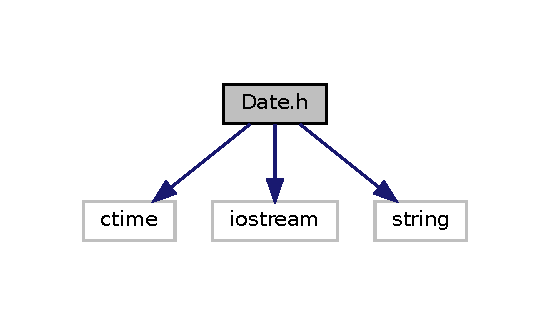
\includegraphics[width=264pt]{Date_8h__incl}
\end{center}
\end{figure}
This graph shows which files directly or indirectly include this file\+:
\nopagebreak
\begin{figure}[H]
\begin{center}
\leavevmode
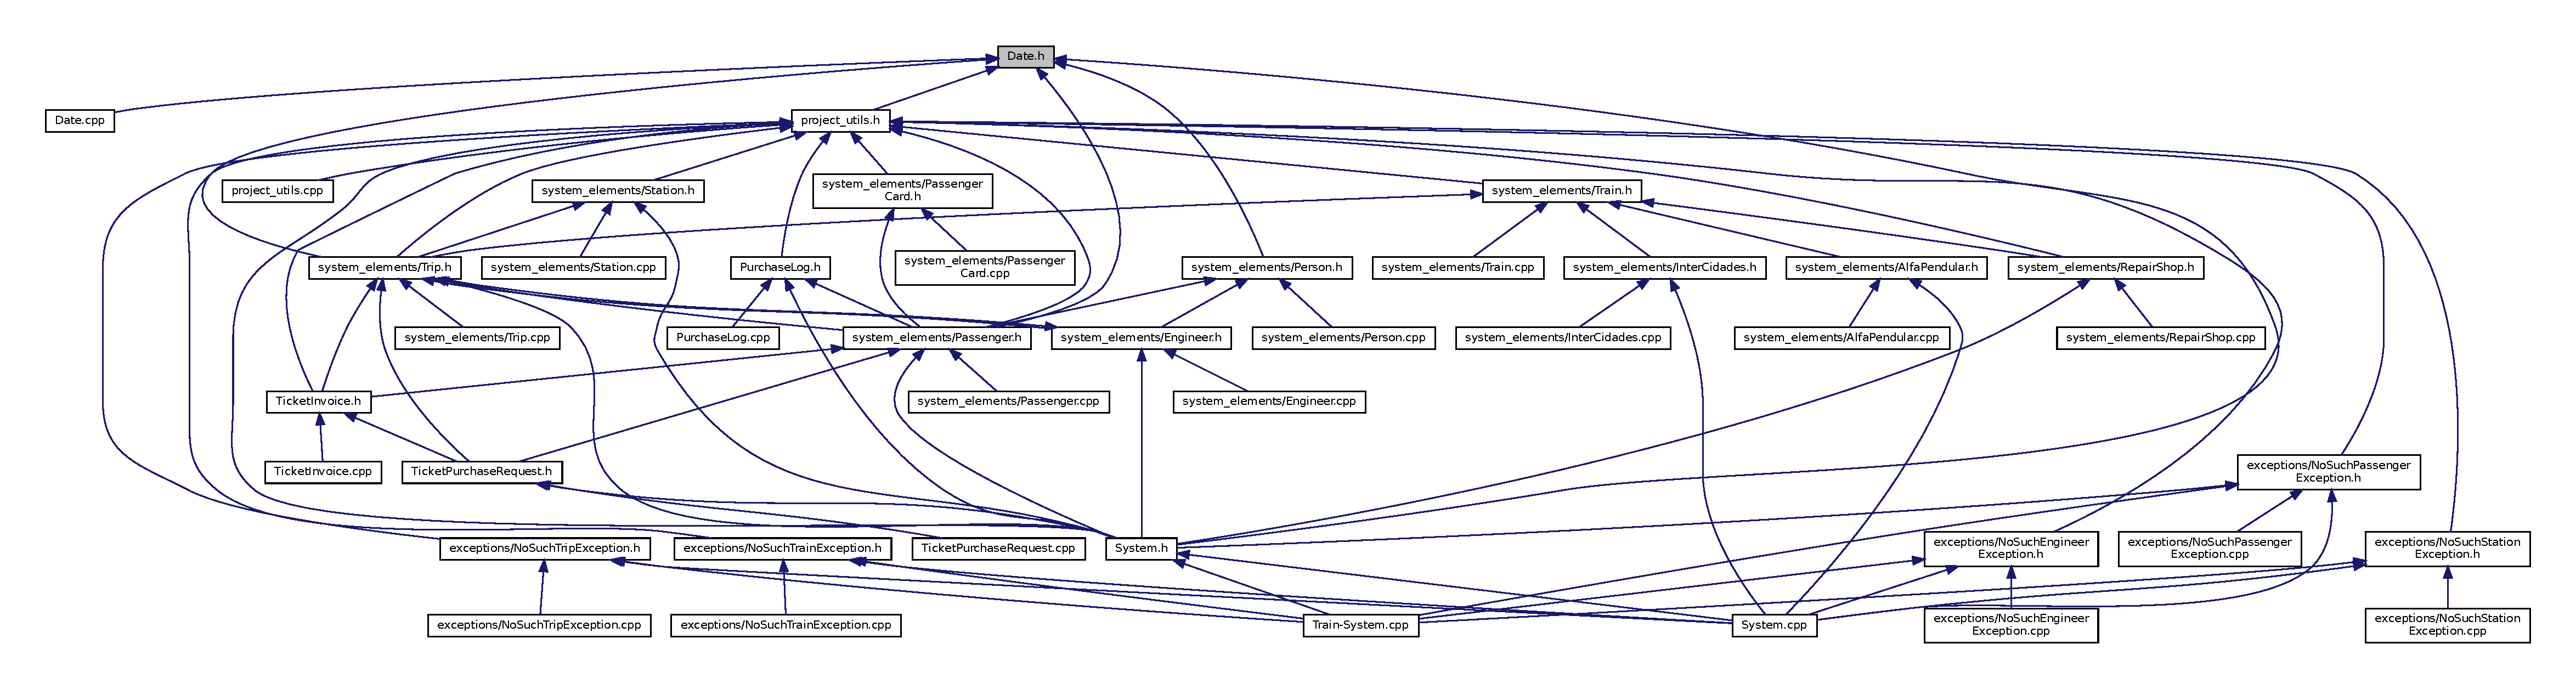
\includegraphics[width=350pt]{Date_8h__dep__incl}
\end{center}
\end{figure}
\subsection*{Classes}
\begin{DoxyCompactItemize}
\item 
class \mbox{\hyperlink{classDate}{Date}}
\begin{DoxyCompactList}\small\item\em Class for representing dates in the program. \end{DoxyCompactList}\end{DoxyCompactItemize}

\hypertarget{IdenticalDestinationException_8cpp}{}\section{exceptions/\+Identical\+Destination\+Exception.cpp File Reference}
\label{IdenticalDestinationException_8cpp}\index{exceptions/\+Identical\+Destination\+Exception.\+cpp@{exceptions/\+Identical\+Destination\+Exception.\+cpp}}
{\ttfamily \#include \char`\"{}Identical\+Destination\+Exception.\+h\char`\"{}}\newline
Include dependency graph for Identical\+Destination\+Exception.\+cpp\+:
\nopagebreak
\begin{figure}[H]
\begin{center}
\leavevmode
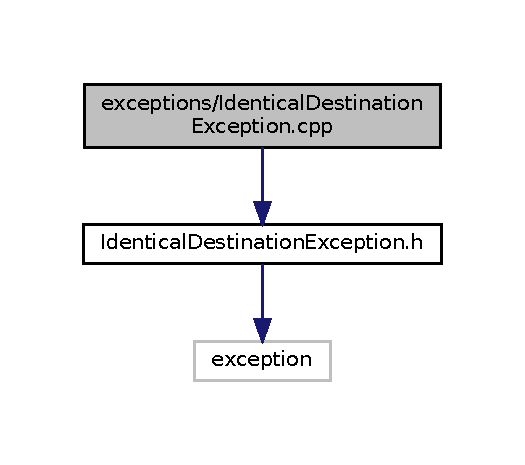
\includegraphics[width=252pt]{IdenticalDestinationException_8cpp__incl}
\end{center}
\end{figure}

\hypertarget{IdenticalDestinationException_8h}{}\section{exceptions/\+Identical\+Destination\+Exception.h File Reference}
\label{IdenticalDestinationException_8h}\index{exceptions/\+Identical\+Destination\+Exception.\+h@{exceptions/\+Identical\+Destination\+Exception.\+h}}
{\ttfamily \#include $<$exception$>$}\newline
Include dependency graph for Identical\+Destination\+Exception.\+h\+:
\nopagebreak
\begin{figure}[H]
\begin{center}
\leavevmode
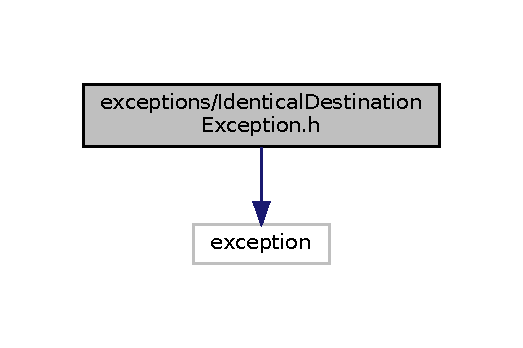
\includegraphics[width=251pt]{IdenticalDestinationException_8h__incl}
\end{center}
\end{figure}
This graph shows which files directly or indirectly include this file\+:
\nopagebreak
\begin{figure}[H]
\begin{center}
\leavevmode
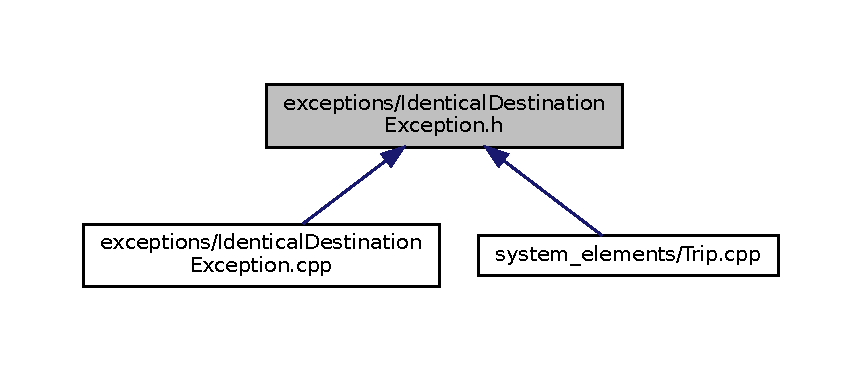
\includegraphics[width=350pt]{IdenticalDestinationException_8h__dep__incl}
\end{center}
\end{figure}
\subsection*{Classes}
\begin{DoxyCompactItemize}
\item 
class \mbox{\hyperlink{classIdenticalDestinationException}{Identical\+Destination\+Exception}}
\begin{DoxyCompactList}\small\item\em Exception reporting when a trip has destination identical to source. \end{DoxyCompactList}\end{DoxyCompactItemize}

\hypertarget{InvalidDateException_8cpp}{}\section{exceptions/\+Invalid\+Date\+Exception.cpp File Reference}
\label{InvalidDateException_8cpp}\index{exceptions/\+Invalid\+Date\+Exception.\+cpp@{exceptions/\+Invalid\+Date\+Exception.\+cpp}}
{\ttfamily \#include \char`\"{}Invalid\+Date\+Exception.\+h\char`\"{}}\newline
{\ttfamily \#include $<$sstream$>$}\newline
Include dependency graph for Invalid\+Date\+Exception.\+cpp\+:
\nopagebreak
\begin{figure}[H]
\begin{center}
\leavevmode
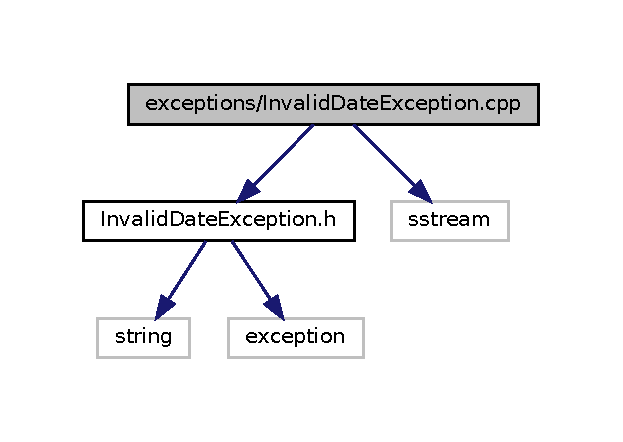
\includegraphics[width=299pt]{InvalidDateException_8cpp__incl}
\end{center}
\end{figure}

\hypertarget{InvalidDateException_8h}{}\section{exceptions/\+Invalid\+Date\+Exception.h File Reference}
\label{InvalidDateException_8h}\index{exceptions/\+Invalid\+Date\+Exception.\+h@{exceptions/\+Invalid\+Date\+Exception.\+h}}
{\ttfamily \#include $<$string$>$}\newline
{\ttfamily \#include $<$exception$>$}\newline
Include dependency graph for Invalid\+Date\+Exception.\+h\+:
\nopagebreak
\begin{figure}[H]
\begin{center}
\leavevmode
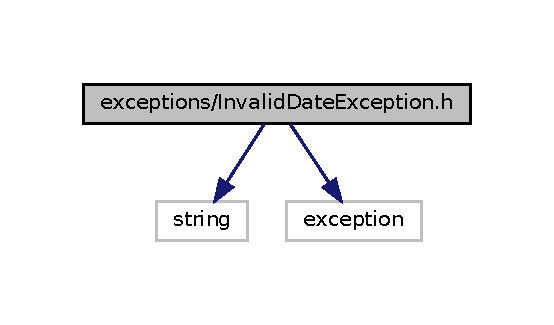
\includegraphics[width=266pt]{InvalidDateException_8h__incl}
\end{center}
\end{figure}
This graph shows which files directly or indirectly include this file\+:
\nopagebreak
\begin{figure}[H]
\begin{center}
\leavevmode
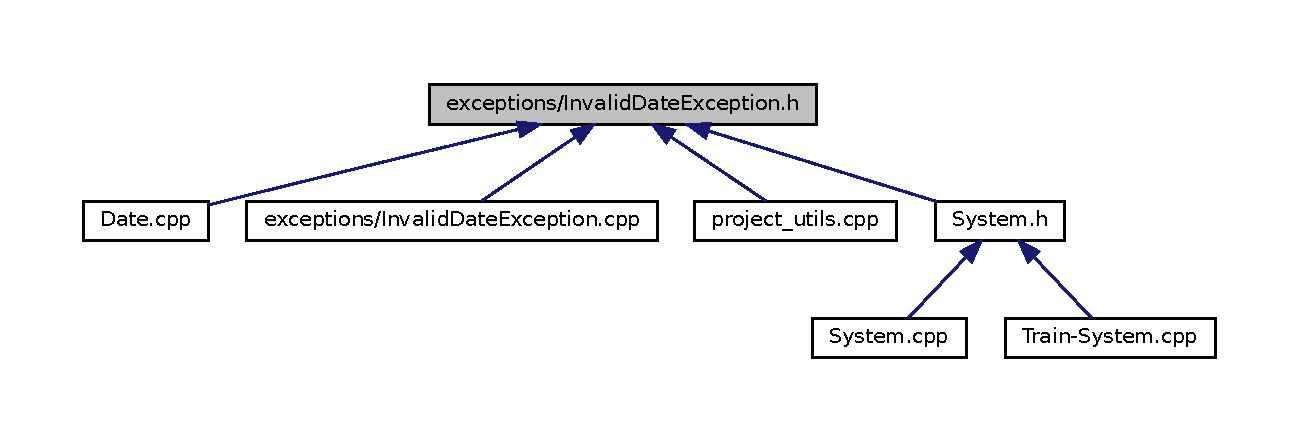
\includegraphics[width=350pt]{InvalidDateException_8h__dep__incl}
\end{center}
\end{figure}
\subsection*{Classes}
\begin{DoxyCompactItemize}
\item 
class \mbox{\hyperlink{classInvalidDateException}{Invalid\+Date\+Exception}}
\begin{DoxyCompactList}\small\item\em Exception reporting an invalid date. \end{DoxyCompactList}\end{DoxyCompactItemize}

\hypertarget{InvalidTrainTypeException_8cpp}{}\section{exceptions/\+Invalid\+Train\+Type\+Exception.cpp File Reference}
\label{InvalidTrainTypeException_8cpp}\index{exceptions/\+Invalid\+Train\+Type\+Exception.\+cpp@{exceptions/\+Invalid\+Train\+Type\+Exception.\+cpp}}
{\ttfamily \#include $<$sstream$>$}\newline
{\ttfamily \#include \char`\"{}Invalid\+Train\+Type\+Exception.\+h\char`\"{}}\newline
Include dependency graph for Invalid\+Train\+Type\+Exception.\+cpp\+:
\nopagebreak
\begin{figure}[H]
\begin{center}
\leavevmode
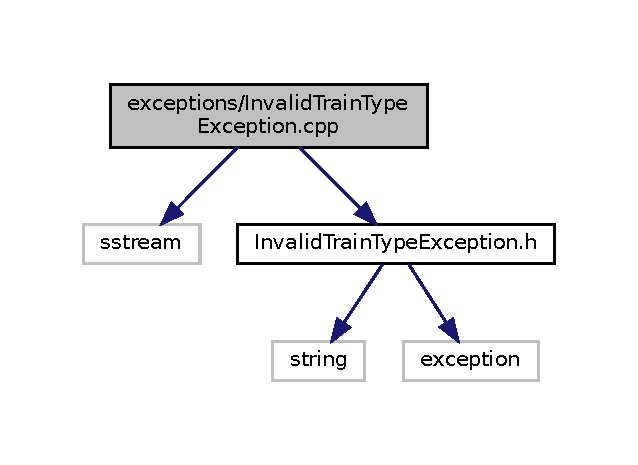
\includegraphics[width=306pt]{InvalidTrainTypeException_8cpp__incl}
\end{center}
\end{figure}

\hypertarget{InvalidTrainTypeException_8h}{}\section{exceptions/\+Invalid\+Train\+Type\+Exception.h File Reference}
\label{InvalidTrainTypeException_8h}\index{exceptions/\+Invalid\+Train\+Type\+Exception.\+h@{exceptions/\+Invalid\+Train\+Type\+Exception.\+h}}
{\ttfamily \#include $<$string$>$}\newline
{\ttfamily \#include $<$exception$>$}\newline
Include dependency graph for Invalid\+Train\+Type\+Exception.\+h\+:
\nopagebreak
\begin{figure}[H]
\begin{center}
\leavevmode
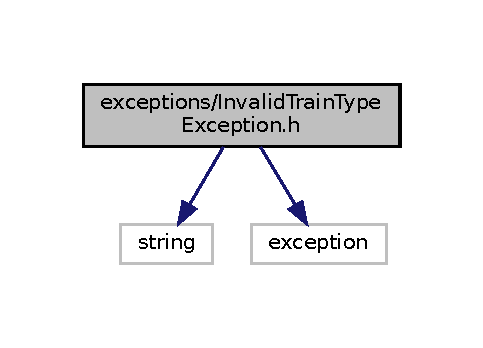
\includegraphics[width=232pt]{InvalidTrainTypeException_8h__incl}
\end{center}
\end{figure}
This graph shows which files directly or indirectly include this file\+:
\nopagebreak
\begin{figure}[H]
\begin{center}
\leavevmode
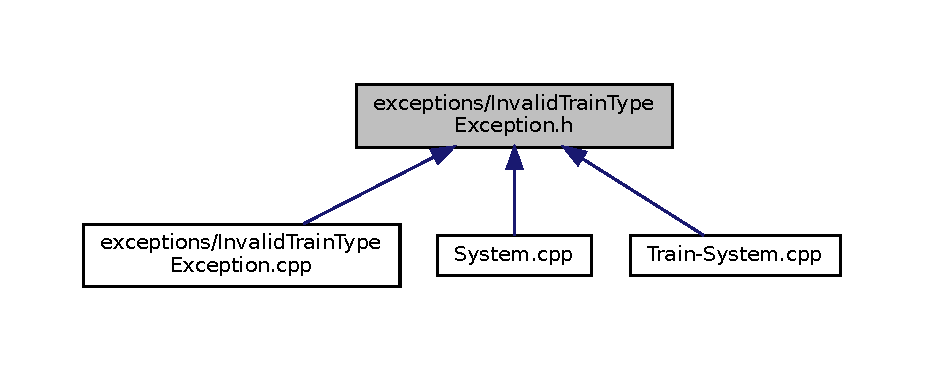
\includegraphics[width=350pt]{InvalidTrainTypeException_8h__dep__incl}
\end{center}
\end{figure}
\subsection*{Classes}
\begin{DoxyCompactItemize}
\item 
class \mbox{\hyperlink{classInvalidTrainTypeException}{Invalid\+Train\+Type\+Exception}}
\end{DoxyCompactItemize}

\hypertarget{NoSuchEngineerException_8cpp}{}\section{exceptions/\+No\+Such\+Engineer\+Exception.cpp File Reference}
\label{NoSuchEngineerException_8cpp}\index{exceptions/\+No\+Such\+Engineer\+Exception.\+cpp@{exceptions/\+No\+Such\+Engineer\+Exception.\+cpp}}
{\ttfamily \#include $<$sstream$>$}\newline
{\ttfamily \#include \char`\"{}No\+Such\+Engineer\+Exception.\+h\char`\"{}}\newline
Include dependency graph for No\+Such\+Engineer\+Exception.\+cpp\+:
\nopagebreak
\begin{figure}[H]
\begin{center}
\leavevmode
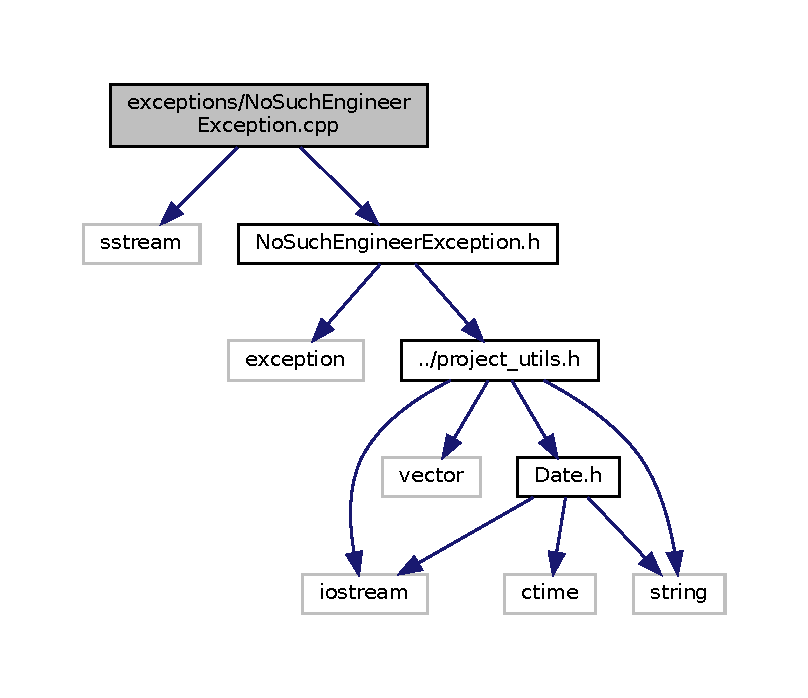
\includegraphics[width=350pt]{NoSuchEngineerException_8cpp__incl}
\end{center}
\end{figure}

\hypertarget{NoSuchEngineerException_8h}{}\section{exceptions/\+No\+Such\+Engineer\+Exception.h File Reference}
\label{NoSuchEngineerException_8h}\index{exceptions/\+No\+Such\+Engineer\+Exception.\+h@{exceptions/\+No\+Such\+Engineer\+Exception.\+h}}
{\ttfamily \#include $<$exception$>$}\newline
{\ttfamily \#include \char`\"{}../project\+\_\+utils.\+h\char`\"{}}\newline
Include dependency graph for No\+Such\+Engineer\+Exception.\+h\+:
\nopagebreak
\begin{figure}[H]
\begin{center}
\leavevmode
\includegraphics[width=319pt]{NoSuchEngineerException_8h__incl}
\end{center}
\end{figure}
This graph shows which files directly or indirectly include this file\+:
\nopagebreak
\begin{figure}[H]
\begin{center}
\leavevmode
\includegraphics[width=350pt]{NoSuchEngineerException_8h__dep__incl}
\end{center}
\end{figure}
\subsection*{Classes}
\begin{DoxyCompactItemize}
\item 
class \mbox{\hyperlink{classNoSuchEngineerException}{No\+Such\+Engineer\+Exception}}
\end{DoxyCompactItemize}

\hypertarget{NoSuchPassengerException_8cpp}{}\section{exceptions/\+No\+Such\+Passenger\+Exception.cpp File Reference}
\label{NoSuchPassengerException_8cpp}\index{exceptions/\+No\+Such\+Passenger\+Exception.\+cpp@{exceptions/\+No\+Such\+Passenger\+Exception.\+cpp}}
{\ttfamily \#include \char`\"{}No\+Such\+Passenger\+Exception.\+h\char`\"{}}\newline
{\ttfamily \#include $<$sstream$>$}\newline
Include dependency graph for No\+Such\+Passenger\+Exception.\+cpp\+:
\nopagebreak
\begin{figure}[H]
\begin{center}
\leavevmode
\includegraphics[width=350pt]{NoSuchPassengerException_8cpp__incl}
\end{center}
\end{figure}

\hypertarget{NoSuchPassengerException_8h}{}\section{exceptions/\+No\+Such\+Passenger\+Exception.h File Reference}
\label{NoSuchPassengerException_8h}\index{exceptions/\+No\+Such\+Passenger\+Exception.\+h@{exceptions/\+No\+Such\+Passenger\+Exception.\+h}}
{\ttfamily \#include \char`\"{}../project\+\_\+utils.\+h\char`\"{}}\newline
{\ttfamily \#include $<$exception$>$}\newline
Include dependency graph for No\+Such\+Passenger\+Exception.\+h\+:
\nopagebreak
\begin{figure}[H]
\begin{center}
\leavevmode
\includegraphics[width=306pt]{NoSuchPassengerException_8h__incl}
\end{center}
\end{figure}
This graph shows which files directly or indirectly include this file\+:
\nopagebreak
\begin{figure}[H]
\begin{center}
\leavevmode
\includegraphics[width=350pt]{NoSuchPassengerException_8h__dep__incl}
\end{center}
\end{figure}
\subsection*{Classes}
\begin{DoxyCompactItemize}
\item 
class \mbox{\hyperlink{classNoSuchPassengerException}{No\+Such\+Passenger\+Exception}}
\begin{DoxyCompactList}\small\item\em Exception reporting that a passenger ID does not exist in the system. \end{DoxyCompactList}\end{DoxyCompactItemize}

\hypertarget{NoSuchStationException_8cpp}{}\section{exceptions/\+No\+Such\+Station\+Exception.cpp File Reference}
\label{NoSuchStationException_8cpp}\index{exceptions/\+No\+Such\+Station\+Exception.\+cpp@{exceptions/\+No\+Such\+Station\+Exception.\+cpp}}
{\ttfamily \#include \char`\"{}No\+Such\+Station\+Exception.\+h\char`\"{}}\newline
{\ttfamily \#include $<$sstream$>$}\newline
Include dependency graph for No\+Such\+Station\+Exception.\+cpp\+:
\nopagebreak
\begin{figure}[H]
\begin{center}
\leavevmode
\includegraphics[width=319pt]{NoSuchStationException_8cpp__incl}
\end{center}
\end{figure}

\hypertarget{NoSuchStationException_8h}{}\section{exceptions/\+No\+Such\+Station\+Exception.h File Reference}
\label{NoSuchStationException_8h}\index{exceptions/\+No\+Such\+Station\+Exception.\+h@{exceptions/\+No\+Such\+Station\+Exception.\+h}}
{\ttfamily \#include $<$exception$>$}\newline
{\ttfamily \#include \char`\"{}../project\+\_\+utils.\+h\char`\"{}}\newline
Include dependency graph for No\+Such\+Station\+Exception.\+h\+:
\nopagebreak
\begin{figure}[H]
\begin{center}
\leavevmode
\includegraphics[width=319pt]{NoSuchStationException_8h__incl}
\end{center}
\end{figure}
This graph shows which files directly or indirectly include this file\+:
\nopagebreak
\begin{figure}[H]
\begin{center}
\leavevmode
\includegraphics[width=350pt]{NoSuchStationException_8h__dep__incl}
\end{center}
\end{figure}
\subsection*{Classes}
\begin{DoxyCompactItemize}
\item 
class \mbox{\hyperlink{classNoSuchStationException}{No\+Such\+Station\+Exception}}
\begin{DoxyCompactList}\small\item\em Exception reporting that a station ID does not exist in the system. \end{DoxyCompactList}\end{DoxyCompactItemize}

\hypertarget{NoSuchTrainException_8cpp}{}\section{exceptions/\+No\+Such\+Train\+Exception.cpp File Reference}
\label{NoSuchTrainException_8cpp}\index{exceptions/\+No\+Such\+Train\+Exception.\+cpp@{exceptions/\+No\+Such\+Train\+Exception.\+cpp}}
{\ttfamily \#include \char`\"{}No\+Such\+Train\+Exception.\+h\char`\"{}}\newline
{\ttfamily \#include $<$sstream$>$}\newline
Include dependency graph for No\+Such\+Train\+Exception.\+cpp\+:
\nopagebreak
\begin{figure}[H]
\begin{center}
\leavevmode
\includegraphics[width=319pt]{NoSuchTrainException_8cpp__incl}
\end{center}
\end{figure}

\hypertarget{NoSuchTrainException_8h}{}\section{exceptions/\+No\+Such\+Train\+Exception.h File Reference}
\label{NoSuchTrainException_8h}\index{exceptions/\+No\+Such\+Train\+Exception.\+h@{exceptions/\+No\+Such\+Train\+Exception.\+h}}
{\ttfamily \#include $<$exception$>$}\newline
{\ttfamily \#include \char`\"{}../project\+\_\+utils.\+h\char`\"{}}\newline
Include dependency graph for No\+Such\+Train\+Exception.\+h\+:
\nopagebreak
\begin{figure}[H]
\begin{center}
\leavevmode
\includegraphics[width=332pt]{NoSuchTrainException_8h__incl}
\end{center}
\end{figure}
This graph shows which files directly or indirectly include this file\+:
\nopagebreak
\begin{figure}[H]
\begin{center}
\leavevmode
\includegraphics[width=350pt]{NoSuchTrainException_8h__dep__incl}
\end{center}
\end{figure}
\subsection*{Classes}
\begin{DoxyCompactItemize}
\item 
class \mbox{\hyperlink{classNoSuchTrainException}{No\+Such\+Train\+Exception}}
\begin{DoxyCompactList}\small\item\em Exception reporting that a train ID does not exist in the system. \end{DoxyCompactList}\end{DoxyCompactItemize}

\hypertarget{NoSuchTripException_8cpp}{}\section{exceptions/\+No\+Such\+Trip\+Exception.cpp File Reference}
\label{NoSuchTripException_8cpp}\index{exceptions/\+No\+Such\+Trip\+Exception.\+cpp@{exceptions/\+No\+Such\+Trip\+Exception.\+cpp}}
{\ttfamily \#include \char`\"{}No\+Such\+Trip\+Exception.\+h\char`\"{}}\newline
{\ttfamily \#include $<$sstream$>$}\newline
Include dependency graph for No\+Such\+Trip\+Exception.\+cpp\+:
\nopagebreak
\begin{figure}[H]
\begin{center}
\leavevmode
\includegraphics[width=319pt]{NoSuchTripException_8cpp__incl}
\end{center}
\end{figure}

\hypertarget{NoSuchTripException_8h}{}\section{exceptions/\+No\+Such\+Trip\+Exception.h File Reference}
\label{NoSuchTripException_8h}\index{exceptions/\+No\+Such\+Trip\+Exception.\+h@{exceptions/\+No\+Such\+Trip\+Exception.\+h}}
{\ttfamily \#include $<$exception$>$}\newline
{\ttfamily \#include \char`\"{}../project\+\_\+utils.\+h\char`\"{}}\newline
Include dependency graph for No\+Such\+Trip\+Exception.\+h\+:
\nopagebreak
\begin{figure}[H]
\begin{center}
\leavevmode
\includegraphics[width=329pt]{NoSuchTripException_8h__incl}
\end{center}
\end{figure}
This graph shows which files directly or indirectly include this file\+:
\nopagebreak
\begin{figure}[H]
\begin{center}
\leavevmode
\includegraphics[width=350pt]{NoSuchTripException_8h__dep__incl}
\end{center}
\end{figure}
\subsection*{Classes}
\begin{DoxyCompactItemize}
\item 
class \mbox{\hyperlink{classNoSuchTripException}{No\+Such\+Trip\+Exception}}
\begin{DoxyCompactList}\small\item\em Exception reporting that a trip ID does not exist in the system. \end{DoxyCompactList}\end{DoxyCompactItemize}

\hypertarget{ReverseDatesException_8cpp}{}\section{exceptions/\+Reverse\+Dates\+Exception.cpp File Reference}
\label{ReverseDatesException_8cpp}\index{exceptions/\+Reverse\+Dates\+Exception.\+cpp@{exceptions/\+Reverse\+Dates\+Exception.\+cpp}}
{\ttfamily \#include \char`\"{}Reverse\+Dates\+Exception.\+h\char`\"{}}\newline
{\ttfamily \#include $<$sstream$>$}\newline
Include dependency graph for Reverse\+Dates\+Exception.\+cpp\+:
\nopagebreak
\begin{figure}[H]
\begin{center}
\leavevmode
\includegraphics[width=314pt]{ReverseDatesException_8cpp__incl}
\end{center}
\end{figure}

\hypertarget{ReverseDatesException_8h}{}\section{exceptions/\+Reverse\+Dates\+Exception.h File Reference}
\label{ReverseDatesException_8h}\index{exceptions/\+Reverse\+Dates\+Exception.\+h@{exceptions/\+Reverse\+Dates\+Exception.\+h}}
{\ttfamily \#include $<$exception$>$}\newline
{\ttfamily \#include $<$string$>$}\newline
Include dependency graph for Reverse\+Dates\+Exception.\+h\+:
\nopagebreak
\begin{figure}[H]
\begin{center}
\leavevmode
\includegraphics[width=278pt]{ReverseDatesException_8h__incl}
\end{center}
\end{figure}
This graph shows which files directly or indirectly include this file\+:
\nopagebreak
\begin{figure}[H]
\begin{center}
\leavevmode
\includegraphics[width=350pt]{ReverseDatesException_8h__dep__incl}
\end{center}
\end{figure}
\subsection*{Classes}
\begin{DoxyCompactItemize}
\item 
class \mbox{\hyperlink{classReverseDatesException}{Reverse\+Dates\+Exception}}
\begin{DoxyCompactList}\small\item\em Exception reporting a trip\textquotesingle{}s arrival date happens before departure date. \end{DoxyCompactList}\end{DoxyCompactItemize}

\hypertarget{TripPastException_8cpp}{}\section{exceptions/\+Trip\+Past\+Exception.cpp File Reference}
\label{TripPastException_8cpp}\index{exceptions/\+Trip\+Past\+Exception.\+cpp@{exceptions/\+Trip\+Past\+Exception.\+cpp}}
{\ttfamily \#include \char`\"{}Trip\+Past\+Exception.\+h\char`\"{}}\newline
Include dependency graph for Trip\+Past\+Exception.\+cpp\+:
\nopagebreak
\begin{figure}[H]
\begin{center}
\leavevmode
\includegraphics[width=259pt]{TripPastException_8cpp__incl}
\end{center}
\end{figure}

\hypertarget{TripPastException_8h}{}\section{exceptions/\+Trip\+Past\+Exception.h File Reference}
\label{TripPastException_8h}\index{exceptions/\+Trip\+Past\+Exception.\+h@{exceptions/\+Trip\+Past\+Exception.\+h}}
{\ttfamily \#include $<$exception$>$}\newline
Include dependency graph for Trip\+Past\+Exception.\+h\+:
\nopagebreak
\begin{figure}[H]
\begin{center}
\leavevmode
\includegraphics[width=248pt]{TripPastException_8h__incl}
\end{center}
\end{figure}
This graph shows which files directly or indirectly include this file\+:
\nopagebreak
\begin{figure}[H]
\begin{center}
\leavevmode
\includegraphics[width=350pt]{TripPastException_8h__dep__incl}
\end{center}
\end{figure}
\subsection*{Classes}
\begin{DoxyCompactItemize}
\item 
class \mbox{\hyperlink{classTripPastException}{Trip\+Past\+Exception}}
\begin{DoxyCompactList}\small\item\em An exception reporting that a trip is already in the past. \end{DoxyCompactList}\end{DoxyCompactItemize}

\hypertarget{project__utils_8cpp}{}\section{project\+\_\+utils.\+cpp File Reference}
\label{project__utils_8cpp}\index{project\+\_\+utils.\+cpp@{project\+\_\+utils.\+cpp}}
{\ttfamily \#include \char`\"{}project\+\_\+utils.\+h\char`\"{}}\newline
{\ttfamily \#include $<$cmath$>$}\newline
{\ttfamily \#include \char`\"{}exceptions/\+Invalid\+Date\+Exception.\+h\char`\"{}}\newline
Include dependency graph for project\+\_\+utils.\+cpp\+:
\nopagebreak
\begin{figure}[H]
\begin{center}
\leavevmode
\includegraphics[width=350pt]{project__utils_8cpp__incl}
\end{center}
\end{figure}

\hypertarget{project__utils_8h}{}\section{project\+\_\+utils.\+h File Reference}
\label{project__utils_8h}\index{project\+\_\+utils.\+h@{project\+\_\+utils.\+h}}
{\ttfamily \#include $<$iostream$>$}\newline
{\ttfamily \#include $<$vector$>$}\newline
{\ttfamily \#include $<$string$>$}\newline
{\ttfamily \#include \char`\"{}Date.\+h\char`\"{}}\newline
Include dependency graph for project\+\_\+utils.\+h\+:
\nopagebreak
\begin{figure}[H]
\begin{center}
\leavevmode
\includegraphics[width=283pt]{project__utils_8h__incl}
\end{center}
\end{figure}
This graph shows which files directly or indirectly include this file\+:
\nopagebreak
\begin{figure}[H]
\begin{center}
\leavevmode
\includegraphics[width=350pt]{project__utils_8h__dep__incl}
\end{center}
\end{figure}
\subsection*{Namespaces}
\begin{DoxyCompactItemize}
\item 
 \mbox{\hyperlink{namespaceproject__utils}{project\+\_\+utils}}
\end{DoxyCompactItemize}
\subsection*{Macros}
\begin{DoxyCompactItemize}
\item 
\#define \mbox{\hyperlink{project__utils_8h_aa6847a750254c8f653bbea118f312359}{F\+O\+U\+R\+T\+Y\+\_\+\+H\+E\+I\+G\+H\+T\+\_\+\+H\+O\+U\+RS}}~172800
\end{DoxyCompactItemize}
\subsection*{Typedefs}
\begin{DoxyCompactItemize}
\item 
typedef unsigned int \mbox{\hyperlink{project__utils_8h_a91ad9478d81a7aaf2593e8d9c3d06a14}{uint}}
\begin{DoxyCompactList}\small\item\em Abreviation for unsigned ints. \end{DoxyCompactList}\item 
typedef unsigned int \mbox{\hyperlink{project__utils_8h_a8f3a969054ad2200720b96e7e23dd4e1}{id\+\_\+t}}
\begin{DoxyCompactList}\small\item\em Contextual typedef for ID\textquotesingle{}s. \end{DoxyCompactList}\end{DoxyCompactItemize}
\subsection*{Functions}
\begin{DoxyCompactItemize}
\item 
{\footnotesize template$<$class T $>$ }\\bool \mbox{\hyperlink{namespaceproject__utils_a72293f22700ff24cdf6663f45ca10c91}{project\+\_\+utils\+::read\+Var}} (T \&var)
\begin{DoxyCompactList}\small\item\em Template function to read any variable from cin. \end{DoxyCompactList}\item 
bool \mbox{\hyperlink{namespaceproject__utils_aab1cf7fd8bfa2074ed3e6fb99fa973dc}{project\+\_\+utils\+::read\+Line}} (string \&s)
\begin{DoxyCompactList}\small\item\em Function to read a string using getline(cin). \end{DoxyCompactList}\item 
\mbox{\hyperlink{classDate}{Date}} \mbox{\hyperlink{namespaceproject__utils_adab6593a2685f866191793214c7c60ce}{project\+\_\+utils\+::read\+Birth\+Date}} ()
\begin{DoxyCompactList}\small\item\em Read a birthdate. \end{DoxyCompactList}\item 
\mbox{\hyperlink{classDate}{Date}} \mbox{\hyperlink{namespaceproject__utils_a747fa96e998a1a6fb365d2512190098e}{project\+\_\+utils\+::read\+Date}} ()
\begin{DoxyCompactList}\small\item\em Read a date. \end{DoxyCompactList}\item 
std\+::vector$<$ std\+::string $>$ \mbox{\hyperlink{namespaceproject__utils_a8a3acf9a2b81c44b525870adb954dcff}{project\+\_\+utils\+::split\+Arguments}} (std\+::string \&command)
\item 
float \mbox{\hyperlink{namespaceproject__utils_ac8764d0b6de158f9eba38a6b517d8cd8}{project\+\_\+utils\+::point\+Distance}} (float x1, float y1, float x2, float y2)
\end{DoxyCompactItemize}


\subsection{Macro Definition Documentation}
\mbox{\Hypertarget{project__utils_8h_aa6847a750254c8f653bbea118f312359}\label{project__utils_8h_aa6847a750254c8f653bbea118f312359}} 
\index{project\+\_\+utils.\+h@{project\+\_\+utils.\+h}!F\+O\+U\+R\+T\+Y\+\_\+\+H\+E\+I\+G\+H\+T\+\_\+\+H\+O\+U\+RS@{F\+O\+U\+R\+T\+Y\+\_\+\+H\+E\+I\+G\+H\+T\+\_\+\+H\+O\+U\+RS}}
\index{F\+O\+U\+R\+T\+Y\+\_\+\+H\+E\+I\+G\+H\+T\+\_\+\+H\+O\+U\+RS@{F\+O\+U\+R\+T\+Y\+\_\+\+H\+E\+I\+G\+H\+T\+\_\+\+H\+O\+U\+RS}!project\+\_\+utils.\+h@{project\+\_\+utils.\+h}}
\subsubsection{\texorpdfstring{F\+O\+U\+R\+T\+Y\+\_\+\+H\+E\+I\+G\+H\+T\+\_\+\+H\+O\+U\+RS}{FOURTY\_HEIGHT\_HOURS}}
{\footnotesize\ttfamily \#define F\+O\+U\+R\+T\+Y\+\_\+\+H\+E\+I\+G\+H\+T\+\_\+\+H\+O\+U\+RS~172800}



\subsection{Typedef Documentation}
\mbox{\Hypertarget{project__utils_8h_a8f3a969054ad2200720b96e7e23dd4e1}\label{project__utils_8h_a8f3a969054ad2200720b96e7e23dd4e1}} 
\index{project\+\_\+utils.\+h@{project\+\_\+utils.\+h}!id\+\_\+t@{id\+\_\+t}}
\index{id\+\_\+t@{id\+\_\+t}!project\+\_\+utils.\+h@{project\+\_\+utils.\+h}}
\subsubsection{\texorpdfstring{id\+\_\+t}{id\_t}}
{\footnotesize\ttfamily typedef unsigned int \mbox{\hyperlink{project__utils_8h_a8f3a969054ad2200720b96e7e23dd4e1}{id\+\_\+t}}}



Contextual typedef for ID\textquotesingle{}s. 

Since I\+Ds are unsigned integers, this typedef helps get rid of mistakes where people might use a signed int for I\+Ds and cause overflow problems. \mbox{\Hypertarget{project__utils_8h_a91ad9478d81a7aaf2593e8d9c3d06a14}\label{project__utils_8h_a91ad9478d81a7aaf2593e8d9c3d06a14}} 
\index{project\+\_\+utils.\+h@{project\+\_\+utils.\+h}!uint@{uint}}
\index{uint@{uint}!project\+\_\+utils.\+h@{project\+\_\+utils.\+h}}
\subsubsection{\texorpdfstring{uint}{uint}}
{\footnotesize\ttfamily typedef unsigned int \mbox{\hyperlink{project__utils_8h_a91ad9478d81a7aaf2593e8d9c3d06a14}{uint}}}



Abreviation for unsigned ints. 


\hypertarget{PurchaseLog_8cpp}{}\section{Purchase\+Log.\+cpp File Reference}
\label{PurchaseLog_8cpp}\index{Purchase\+Log.\+cpp@{Purchase\+Log.\+cpp}}
{\ttfamily \#include \char`\"{}Purchase\+Log.\+h\char`\"{}}\newline
Include dependency graph for Purchase\+Log.\+cpp\+:
\nopagebreak
\begin{figure}[H]
\begin{center}
\leavevmode
\includegraphics[width=320pt]{PurchaseLog_8cpp__incl}
\end{center}
\end{figure}
\subsection*{Functions}
\begin{DoxyCompactItemize}
\item 
ostream \& \mbox{\hyperlink{PurchaseLog_8cpp_a6e491e1f9d6ee6a67a68c8ba78df6607}{operator$<$$<$}} (ostream \&os, \mbox{\hyperlink{classPurchaseLog}{Purchase\+Log}} \&pl)
\end{DoxyCompactItemize}


\subsection{Function Documentation}
\mbox{\Hypertarget{PurchaseLog_8cpp_a6e491e1f9d6ee6a67a68c8ba78df6607}\label{PurchaseLog_8cpp_a6e491e1f9d6ee6a67a68c8ba78df6607}} 
\index{Purchase\+Log.\+cpp@{Purchase\+Log.\+cpp}!operator$<$$<$@{operator$<$$<$}}
\index{operator$<$$<$@{operator$<$$<$}!Purchase\+Log.\+cpp@{Purchase\+Log.\+cpp}}
\subsubsection{\texorpdfstring{operator$<$$<$()}{operator<<()}}
{\footnotesize\ttfamily ostream\& operator$<$$<$ (\begin{DoxyParamCaption}\item[{ostream \&}]{os,  }\item[{\mbox{\hyperlink{classPurchaseLog}{Purchase\+Log}} \&}]{pl }\end{DoxyParamCaption})}


\hypertarget{PurchaseLog_8h}{}\section{Purchase\+Log.\+h File Reference}
\label{PurchaseLog_8h}\index{Purchase\+Log.\+h@{Purchase\+Log.\+h}}
{\ttfamily \#include $<$iostream$>$}\newline
{\ttfamily \#include $<$string$>$}\newline
{\ttfamily \#include \char`\"{}project\+\_\+utils.\+h\char`\"{}}\newline
Include dependency graph for Purchase\+Log.\+h\+:
\nopagebreak
\begin{figure}[H]
\begin{center}
\leavevmode
\includegraphics[width=320pt]{PurchaseLog_8h__incl}
\end{center}
\end{figure}
This graph shows which files directly or indirectly include this file\+:
\nopagebreak
\begin{figure}[H]
\begin{center}
\leavevmode
\includegraphics[width=350pt]{PurchaseLog_8h__dep__incl}
\end{center}
\end{figure}
\subsection*{Classes}
\begin{DoxyCompactItemize}
\item 
class \mbox{\hyperlink{classPurchaseLog}{Purchase\+Log}}
\begin{DoxyCompactList}\small\item\em A class representing the log of a trip tiket purchase. \end{DoxyCompactList}\end{DoxyCompactItemize}

\hypertarget{System_8cpp}{}\section{System.\+cpp File Reference}
\label{System_8cpp}\index{System.\+cpp@{System.\+cpp}}
{\ttfamily \#include $<$fstream$>$}\newline
{\ttfamily \#include \char`\"{}System.\+h\char`\"{}}\newline
{\ttfamily \#include \char`\"{}exceptions/\+No\+Such\+Passenger\+Exception.\+h\char`\"{}}\newline
{\ttfamily \#include \char`\"{}exceptions/\+No\+Such\+Station\+Exception.\+h\char`\"{}}\newline
{\ttfamily \#include \char`\"{}exceptions/\+No\+Such\+Train\+Exception.\+h\char`\"{}}\newline
{\ttfamily \#include \char`\"{}exceptions/\+No\+Such\+Trip\+Exception.\+h\char`\"{}}\newline
{\ttfamily \#include \char`\"{}exceptions/\+Trip\+Past\+Exception.\+h\char`\"{}}\newline
{\ttfamily \#include \char`\"{}exceptions/\+No\+Such\+Engineer\+Exception.\+h\char`\"{}}\newline
{\ttfamily \#include \char`\"{}system\+\_\+elements/\+Alfa\+Pendular.\+h\char`\"{}}\newline
{\ttfamily \#include \char`\"{}system\+\_\+elements/\+Inter\+Cidades.\+h\char`\"{}}\newline
{\ttfamily \#include \char`\"{}exceptions/\+Invalid\+Train\+Type\+Exception.\+h\char`\"{}}\newline
{\ttfamily \#include $<$algorithm$>$}\newline
{\ttfamily \#include $<$iomanip$>$}\newline
{\ttfamily \#include $<$ctime$>$}\newline
Include dependency graph for System.\+cpp\+:
\nopagebreak
\begin{figure}[H]
\begin{center}
\leavevmode
\includegraphics[width=350pt]{System_8cpp__incl}
\end{center}
\end{figure}
\subsection*{Functions}
\begin{DoxyCompactItemize}
\item 
ostream \& \mbox{\hyperlink{System_8cpp_a5a0b8c727aa046ae23dfe36ce4d5a120}{operator$<$$<$}} (ostream \&os, \mbox{\hyperlink{classSystem}{System}} \&sys)
\end{DoxyCompactItemize}


\subsection{Function Documentation}
\mbox{\Hypertarget{System_8cpp_a5a0b8c727aa046ae23dfe36ce4d5a120}\label{System_8cpp_a5a0b8c727aa046ae23dfe36ce4d5a120}} 
\index{System.\+cpp@{System.\+cpp}!operator$<$$<$@{operator$<$$<$}}
\index{operator$<$$<$@{operator$<$$<$}!System.\+cpp@{System.\+cpp}}
\subsubsection{\texorpdfstring{operator$<$$<$()}{operator<<()}}
{\footnotesize\ttfamily ostream\& operator$<$$<$ (\begin{DoxyParamCaption}\item[{ostream \&}]{os,  }\item[{\mbox{\hyperlink{classSystem}{System}} \&}]{sys }\end{DoxyParamCaption})}

Here is the call graph for this function\+:
\nopagebreak
\begin{figure}[H]
\begin{center}
\leavevmode
\includegraphics[width=327pt]{System_8cpp_a5a0b8c727aa046ae23dfe36ce4d5a120_cgraph}
\end{center}
\end{figure}

\hypertarget{System_8h}{}\section{System.\+h File Reference}
\label{System_8h}\index{System.\+h@{System.\+h}}
{\ttfamily \#include $<$map$>$}\newline
{\ttfamily \#include $<$vector$>$}\newline
{\ttfamily \#include $<$iostream$>$}\newline
{\ttfamily \#include $<$unordered\+\_\+set$>$}\newline
{\ttfamily \#include \char`\"{}system\+\_\+elements/\+Passenger.\+h\char`\"{}}\newline
{\ttfamily \#include \char`\"{}system\+\_\+elements/\+Trip.\+h\char`\"{}}\newline
{\ttfamily \#include \char`\"{}system\+\_\+elements/\+Station.\+h\char`\"{}}\newline
{\ttfamily \#include \char`\"{}Ticket\+Purchase\+Request.\+h\char`\"{}}\newline
{\ttfamily \#include \char`\"{}Date.\+h\char`\"{}}\newline
{\ttfamily \#include \char`\"{}exceptions/\+Invalid\+Date\+Exception.\+h\char`\"{}}\newline
{\ttfamily \#include \char`\"{}project\+\_\+utils.\+h\char`\"{}}\newline
{\ttfamily \#include \char`\"{}Purchase\+Log.\+h\char`\"{}}\newline
{\ttfamily \#include \char`\"{}exceptions/\+No\+Such\+Passenger\+Exception.\+h\char`\"{}}\newline
{\ttfamily \#include \char`\"{}system\+\_\+elements/\+Engineer.\+h\char`\"{}}\newline
{\ttfamily \#include \char`\"{}system\+\_\+elements/\+Repair\+Shop.\+h\char`\"{}}\newline
Include dependency graph for System.\+h\+:
\nopagebreak
\begin{figure}[H]
\begin{center}
\leavevmode
\includegraphics[width=350pt]{System_8h__incl}
\end{center}
\end{figure}
This graph shows which files directly or indirectly include this file\+:
\nopagebreak
\begin{figure}[H]
\begin{center}
\leavevmode
\includegraphics[width=274pt]{System_8h__dep__incl}
\end{center}
\end{figure}
\subsection*{Classes}
\begin{DoxyCompactItemize}
\item 
class \mbox{\hyperlink{classSystem}{System}}
\begin{DoxyCompactList}\small\item\em Class to represent the central system. \end{DoxyCompactList}\end{DoxyCompactItemize}

\hypertarget{AlfaPendular_8cpp}{}\section{system\+\_\+elements/\+Alfa\+Pendular.cpp File Reference}
\label{AlfaPendular_8cpp}\index{system\+\_\+elements/\+Alfa\+Pendular.\+cpp@{system\+\_\+elements/\+Alfa\+Pendular.\+cpp}}
{\ttfamily \#include $<$iomanip$>$}\newline
{\ttfamily \#include \char`\"{}Alfa\+Pendular.\+h\char`\"{}}\newline
Include dependency graph for Alfa\+Pendular.\+cpp\+:
\nopagebreak
\begin{figure}[H]
\begin{center}
\leavevmode
\includegraphics[width=350pt]{AlfaPendular_8cpp__incl}
\end{center}
\end{figure}

\hypertarget{AlfaPendular_8h}{}\section{system\+\_\+elements/\+Alfa\+Pendular.h File Reference}
\label{AlfaPendular_8h}\index{system\+\_\+elements/\+Alfa\+Pendular.\+h@{system\+\_\+elements/\+Alfa\+Pendular.\+h}}
{\ttfamily \#include \char`\"{}Train.\+h\char`\"{}}\newline
Include dependency graph for Alfa\+Pendular.\+h\+:
\nopagebreak
\begin{figure}[H]
\begin{center}
\leavevmode
\includegraphics[width=350pt]{AlfaPendular_8h__incl}
\end{center}
\end{figure}
This graph shows which files directly or indirectly include this file\+:
\nopagebreak
\begin{figure}[H]
\begin{center}
\leavevmode
\includegraphics[width=350pt]{AlfaPendular_8h__dep__incl}
\end{center}
\end{figure}
\subsection*{Classes}
\begin{DoxyCompactItemize}
\item 
class \mbox{\hyperlink{classAlfaPendular}{Alfa\+Pendular}}
\end{DoxyCompactItemize}

\hypertarget{Engineer_8cpp}{}\section{system\+\_\+elements/\+Engineer.cpp File Reference}
\label{Engineer_8cpp}\index{system\+\_\+elements/\+Engineer.\+cpp@{system\+\_\+elements/\+Engineer.\+cpp}}
{\ttfamily \#include \char`\"{}Engineer.\+h\char`\"{}}\newline
{\ttfamily \#include $<$iomanip$>$}\newline
Include dependency graph for Engineer.\+cpp\+:
\nopagebreak
\begin{figure}[H]
\begin{center}
\leavevmode
\includegraphics[width=350pt]{Engineer_8cpp__incl}
\end{center}
\end{figure}

\hypertarget{Engineer_8h}{}\section{system\+\_\+elements/\+Engineer.h File Reference}
\label{Engineer_8h}\index{system\+\_\+elements/\+Engineer.\+h@{system\+\_\+elements/\+Engineer.\+h}}
{\ttfamily \#include $<$set$>$}\newline
{\ttfamily \#include \char`\"{}Person.\+h\char`\"{}}\newline
{\ttfamily \#include \char`\"{}Trip.\+h\char`\"{}}\newline
Include dependency graph for Engineer.\+h\+:
\nopagebreak
\begin{figure}[H]
\begin{center}
\leavevmode
\includegraphics[width=350pt]{Engineer_8h__incl}
\end{center}
\end{figure}
This graph shows which files directly or indirectly include this file\+:
\nopagebreak
\begin{figure}[H]
\begin{center}
\leavevmode
\includegraphics[width=350pt]{Engineer_8h__dep__incl}
\end{center}
\end{figure}
\subsection*{Classes}
\begin{DoxyCompactItemize}
\item 
class \mbox{\hyperlink{classEngineer}{Engineer}}
\item 
struct \mbox{\hyperlink{structEngineer_1_1EngineerHashUtils}{Engineer\+::\+Engineer\+Hash\+Utils}}
\end{DoxyCompactItemize}

\hypertarget{InterCidades_8cpp}{}\section{system\+\_\+elements/\+Inter\+Cidades.cpp File Reference}
\label{InterCidades_8cpp}\index{system\+\_\+elements/\+Inter\+Cidades.\+cpp@{system\+\_\+elements/\+Inter\+Cidades.\+cpp}}
{\ttfamily \#include $<$iomanip$>$}\newline
{\ttfamily \#include \char`\"{}Inter\+Cidades.\+h\char`\"{}}\newline
Include dependency graph for Inter\+Cidades.\+cpp\+:
\nopagebreak
\begin{figure}[H]
\begin{center}
\leavevmode
\includegraphics[width=350pt]{InterCidades_8cpp__incl}
\end{center}
\end{figure}

\hypertarget{InterCidades_8h}{}\section{system\+\_\+elements/\+Inter\+Cidades.h File Reference}
\label{InterCidades_8h}\index{system\+\_\+elements/\+Inter\+Cidades.\+h@{system\+\_\+elements/\+Inter\+Cidades.\+h}}
{\ttfamily \#include \char`\"{}Train.\+h\char`\"{}}\newline
Include dependency graph for Inter\+Cidades.\+h\+:
\nopagebreak
\begin{figure}[H]
\begin{center}
\leavevmode
\includegraphics[width=350pt]{InterCidades_8h__incl}
\end{center}
\end{figure}
This graph shows which files directly or indirectly include this file\+:
\nopagebreak
\begin{figure}[H]
\begin{center}
\leavevmode
\includegraphics[width=350pt]{InterCidades_8h__dep__incl}
\end{center}
\end{figure}
\subsection*{Classes}
\begin{DoxyCompactItemize}
\item 
class \mbox{\hyperlink{classInterCidades}{Inter\+Cidades}}
\end{DoxyCompactItemize}

\hypertarget{Passenger_8cpp}{}\section{system\+\_\+elements/\+Passenger.cpp File Reference}
\label{Passenger_8cpp}\index{system\+\_\+elements/\+Passenger.\+cpp@{system\+\_\+elements/\+Passenger.\+cpp}}
{\ttfamily \#include \char`\"{}Passenger.\+h\char`\"{}}\newline
{\ttfamily \#include $<$iomanip$>$}\newline
Include dependency graph for Passenger.\+cpp\+:
\nopagebreak
\begin{figure}[H]
\begin{center}
\leavevmode
\includegraphics[width=350pt]{Passenger_8cpp__incl}
\end{center}
\end{figure}
\subsection*{Functions}
\begin{DoxyCompactItemize}
\item 
ostream \& \mbox{\hyperlink{Passenger_8cpp_a8a58348a0b4dbb26c2ce2289ba3cb234}{operator$<$$<$}} (ostream \&os, \mbox{\hyperlink{classPassenger}{Passenger}} \&p)
\end{DoxyCompactItemize}


\subsection{Function Documentation}
\mbox{\Hypertarget{Passenger_8cpp_a8a58348a0b4dbb26c2ce2289ba3cb234}\label{Passenger_8cpp_a8a58348a0b4dbb26c2ce2289ba3cb234}} 
\index{Passenger.\+cpp@{Passenger.\+cpp}!operator$<$$<$@{operator$<$$<$}}
\index{operator$<$$<$@{operator$<$$<$}!Passenger.\+cpp@{Passenger.\+cpp}}
\subsubsection{\texorpdfstring{operator$<$$<$()}{operator<<()}}
{\footnotesize\ttfamily ostream\& operator$<$$<$ (\begin{DoxyParamCaption}\item[{ostream \&}]{os,  }\item[{\mbox{\hyperlink{classPassenger}{Passenger}} \&}]{p }\end{DoxyParamCaption})}

Here is the call graph for this function\+:
\nopagebreak
\begin{figure}[H]
\begin{center}
\leavevmode
\includegraphics[width=344pt]{Passenger_8cpp_a8a58348a0b4dbb26c2ce2289ba3cb234_cgraph}
\end{center}
\end{figure}

\hypertarget{Passenger_8h}{}\section{system\+\_\+elements/\+Passenger.h File Reference}
\label{Passenger_8h}\index{system\+\_\+elements/\+Passenger.\+h@{system\+\_\+elements/\+Passenger.\+h}}
{\ttfamily \#include \char`\"{}Person.\+h\char`\"{}}\newline
{\ttfamily \#include \char`\"{}../\+Date.\+h\char`\"{}}\newline
{\ttfamily \#include \char`\"{}Trip.\+h\char`\"{}}\newline
{\ttfamily \#include \char`\"{}Passenger\+Card.\+h\char`\"{}}\newline
{\ttfamily \#include \char`\"{}../project\+\_\+utils.\+h\char`\"{}}\newline
{\ttfamily \#include $<$string$>$}\newline
{\ttfamily \#include $<$vector$>$}\newline
{\ttfamily \#include $<$iostream$>$}\newline
{\ttfamily \#include \char`\"{}../\+Purchase\+Log.\+h\char`\"{}}\newline
Include dependency graph for Passenger.\+h\+:
\nopagebreak
\begin{figure}[H]
\begin{center}
\leavevmode
\includegraphics[width=350pt]{Passenger_8h__incl}
\end{center}
\end{figure}
This graph shows which files directly or indirectly include this file\+:
\nopagebreak
\begin{figure}[H]
\begin{center}
\leavevmode
\includegraphics[width=350pt]{Passenger_8h__dep__incl}
\end{center}
\end{figure}
\subsection*{Classes}
\begin{DoxyCompactItemize}
\item 
class \mbox{\hyperlink{classPassenger}{Passenger}}
\begin{DoxyCompactList}\small\item\em Class for representing a passenger in the system Extends class \mbox{\hyperlink{classPerson}{Person}}. \end{DoxyCompactList}\end{DoxyCompactItemize}

\hypertarget{PassengerCard_8cpp}{}\section{system\+\_\+elements/\+Passenger\+Card.cpp File Reference}
\label{PassengerCard_8cpp}\index{system\+\_\+elements/\+Passenger\+Card.\+cpp@{system\+\_\+elements/\+Passenger\+Card.\+cpp}}
{\ttfamily \#include \char`\"{}Passenger\+Card.\+h\char`\"{}}\newline
Include dependency graph for Passenger\+Card.\+cpp\+:
\nopagebreak
\begin{figure}[H]
\begin{center}
\leavevmode
\includegraphics[width=350pt]{PassengerCard_8cpp__incl}
\end{center}
\end{figure}

\hypertarget{PassengerCard_8h}{}\section{system\+\_\+elements/\+Passenger\+Card.h File Reference}
\label{PassengerCard_8h}\index{system\+\_\+elements/\+Passenger\+Card.\+h@{system\+\_\+elements/\+Passenger\+Card.\+h}}
{\ttfamily \#include \char`\"{}../project\+\_\+utils.\+h\char`\"{}}\newline
{\ttfamily \#include $<$string$>$}\newline
Include dependency graph for Passenger\+Card.\+h\+:
\nopagebreak
\begin{figure}[H]
\begin{center}
\leavevmode
\includegraphics[width=350pt]{PassengerCard_8h__incl}
\end{center}
\end{figure}
This graph shows which files directly or indirectly include this file\+:
\nopagebreak
\begin{figure}[H]
\begin{center}
\leavevmode
\includegraphics[width=350pt]{PassengerCard_8h__dep__incl}
\end{center}
\end{figure}
\subsection*{Classes}
\begin{DoxyCompactItemize}
\item 
class \mbox{\hyperlink{classPassengerCard}{Passenger\+Card}}
\begin{DoxyCompactList}\small\item\em Class for representing the card of a passenger in the system. \end{DoxyCompactList}\end{DoxyCompactItemize}

\hypertarget{Person_8cpp}{}\section{system\+\_\+elements/\+Person.cpp File Reference}
\label{Person_8cpp}\index{system\+\_\+elements/\+Person.\+cpp@{system\+\_\+elements/\+Person.\+cpp}}
{\ttfamily \#include \char`\"{}Person.\+h\char`\"{}}\newline
Include dependency graph for Person.\+cpp\+:
\nopagebreak
\begin{figure}[H]
\begin{center}
\leavevmode
\includegraphics[width=324pt]{Person_8cpp__incl}
\end{center}
\end{figure}

\hypertarget{Person_8h}{}\section{system\+\_\+elements/\+Person.h File Reference}
\label{Person_8h}\index{system\+\_\+elements/\+Person.\+h@{system\+\_\+elements/\+Person.\+h}}
{\ttfamily \#include $<$string$>$}\newline
{\ttfamily \#include \char`\"{}System\+Element.\+h\char`\"{}}\newline
{\ttfamily \#include \char`\"{}../\+Date.\+h\char`\"{}}\newline
Include dependency graph for Person.\+h\+:
\nopagebreak
\begin{figure}[H]
\begin{center}
\leavevmode
\includegraphics[width=319pt]{Person_8h__incl}
\end{center}
\end{figure}
This graph shows which files directly or indirectly include this file\+:
\nopagebreak
\begin{figure}[H]
\begin{center}
\leavevmode
\includegraphics[width=350pt]{Person_8h__dep__incl}
\end{center}
\end{figure}
\subsection*{Classes}
\begin{DoxyCompactItemize}
\item 
class \mbox{\hyperlink{classPerson}{Person}}
\end{DoxyCompactItemize}

\hypertarget{RepairShop_8cpp}{}\section{system\+\_\+elements/\+Repair\+Shop.cpp File Reference}
\label{RepairShop_8cpp}\index{system\+\_\+elements/\+Repair\+Shop.\+cpp@{system\+\_\+elements/\+Repair\+Shop.\+cpp}}
{\ttfamily \#include \char`\"{}Repair\+Shop.\+h\char`\"{}}\newline
{\ttfamily \#include $<$iomanip$>$}\newline
Include dependency graph for Repair\+Shop.\+cpp\+:
\nopagebreak
\begin{figure}[H]
\begin{center}
\leavevmode
\includegraphics[width=350pt]{RepairShop_8cpp__incl}
\end{center}
\end{figure}

\hypertarget{RepairShop_8h}{}\section{system\+\_\+elements/\+Repair\+Shop.h File Reference}
\label{RepairShop_8h}\index{system\+\_\+elements/\+Repair\+Shop.\+h@{system\+\_\+elements/\+Repair\+Shop.\+h}}
{\ttfamily \#include $<$string$>$}\newline
{\ttfamily \#include $<$queue$>$}\newline
{\ttfamily \#include $<$set$>$}\newline
{\ttfamily \#include $<$fstream$>$}\newline
{\ttfamily \#include \char`\"{}System\+Element.\+h\char`\"{}}\newline
{\ttfamily \#include \char`\"{}../project\+\_\+utils.\+h\char`\"{}}\newline
{\ttfamily \#include \char`\"{}Train.\+h\char`\"{}}\newline
Include dependency graph for Repair\+Shop.\+h\+:
\nopagebreak
\begin{figure}[H]
\begin{center}
\leavevmode
\includegraphics[width=350pt]{RepairShop_8h__incl}
\end{center}
\end{figure}
This graph shows which files directly or indirectly include this file\+:
\nopagebreak
\begin{figure}[H]
\begin{center}
\leavevmode
\includegraphics[width=350pt]{RepairShop_8h__dep__incl}
\end{center}
\end{figure}
\subsection*{Classes}
\begin{DoxyCompactItemize}
\item 
class \mbox{\hyperlink{classRepairShop}{Repair\+Shop}}
\item 
struct \mbox{\hyperlink{structRepairShop_1_1RepairShopPQUtils}{Repair\+Shop\+::\+Repair\+Shop\+P\+Q\+Utils}}
\end{DoxyCompactItemize}

\hypertarget{Station_8cpp}{}\section{system\+\_\+elements/\+Station.cpp File Reference}
\label{Station_8cpp}\index{system\+\_\+elements/\+Station.\+cpp@{system\+\_\+elements/\+Station.\+cpp}}
{\ttfamily \#include \char`\"{}Station.\+h\char`\"{}}\newline
{\ttfamily \#include $<$iomanip$>$}\newline
Include dependency graph for Station.\+cpp\+:
\nopagebreak
\begin{figure}[H]
\begin{center}
\leavevmode
\includegraphics[width=350pt]{Station_8cpp__incl}
\end{center}
\end{figure}
\subsection*{Functions}
\begin{DoxyCompactItemize}
\item 
ostream \& \mbox{\hyperlink{Station_8cpp_a3a0abc644a8c0bb1bd113b6938adff3d}{operator$<$$<$}} (ostream \&os, \mbox{\hyperlink{classStation}{Station}} \&st)
\end{DoxyCompactItemize}


\subsection{Function Documentation}
\mbox{\Hypertarget{Station_8cpp_a3a0abc644a8c0bb1bd113b6938adff3d}\label{Station_8cpp_a3a0abc644a8c0bb1bd113b6938adff3d}} 
\index{Station.\+cpp@{Station.\+cpp}!operator$<$$<$@{operator$<$$<$}}
\index{operator$<$$<$@{operator$<$$<$}!Station.\+cpp@{Station.\+cpp}}
\subsubsection{\texorpdfstring{operator$<$$<$()}{operator<<()}}
{\footnotesize\ttfamily ostream\& operator$<$$<$ (\begin{DoxyParamCaption}\item[{ostream \&}]{os,  }\item[{\mbox{\hyperlink{classStation}{Station}} \&}]{st }\end{DoxyParamCaption})}


\hypertarget{Station_8h}{}\section{system\+\_\+elements/\+Station.h File Reference}
\label{Station_8h}\index{system\+\_\+elements/\+Station.\+h@{system\+\_\+elements/\+Station.\+h}}
{\ttfamily \#include \char`\"{}System\+Element.\+h\char`\"{}}\newline
{\ttfamily \#include \char`\"{}../project\+\_\+utils.\+h\char`\"{}}\newline
{\ttfamily \#include $<$string$>$}\newline
{\ttfamily \#include $<$iostream$>$}\newline
Include dependency graph for Station.\+h\+:
\nopagebreak
\begin{figure}[H]
\begin{center}
\leavevmode
\includegraphics[width=350pt]{Station_8h__incl}
\end{center}
\end{figure}
This graph shows which files directly or indirectly include this file\+:
\nopagebreak
\begin{figure}[H]
\begin{center}
\leavevmode
\includegraphics[width=350pt]{Station_8h__dep__incl}
\end{center}
\end{figure}
\subsection*{Classes}
\begin{DoxyCompactItemize}
\item 
class \mbox{\hyperlink{classStation}{Station}}
\begin{DoxyCompactList}\small\item\em Class for representing a station in the system. \end{DoxyCompactList}\end{DoxyCompactItemize}

\hypertarget{SystemElement_8cpp}{}\section{system\+\_\+elements/\+System\+Element.cpp File Reference}
\label{SystemElement_8cpp}\index{system\+\_\+elements/\+System\+Element.\+cpp@{system\+\_\+elements/\+System\+Element.\+cpp}}
{\ttfamily \#include \char`\"{}System\+Element.\+h\char`\"{}}\newline
Include dependency graph for System\+Element.\+cpp\+:
\nopagebreak
\begin{figure}[H]
\begin{center}
\leavevmode
\includegraphics[width=284pt]{SystemElement_8cpp__incl}
\end{center}
\end{figure}

\hypertarget{SystemElement_8h}{}\section{system\+\_\+elements/\+System\+Element.h File Reference}
\label{SystemElement_8h}\index{system\+\_\+elements/\+System\+Element.\+h@{system\+\_\+elements/\+System\+Element.\+h}}
This graph shows which files directly or indirectly include this file\+:
\nopagebreak
\begin{figure}[H]
\begin{center}
\leavevmode
\includegraphics[width=350pt]{SystemElement_8h__dep__incl}
\end{center}
\end{figure}
\subsection*{Classes}
\begin{DoxyCompactItemize}
\item 
class \mbox{\hyperlink{classSystemElement}{System\+Element}}
\end{DoxyCompactItemize}

\hypertarget{Train_8cpp}{}\section{system\+\_\+elements/\+Train.cpp File Reference}
\label{Train_8cpp}\index{system\+\_\+elements/\+Train.\+cpp@{system\+\_\+elements/\+Train.\+cpp}}
{\ttfamily \#include \char`\"{}Train.\+h\char`\"{}}\newline
{\ttfamily \#include $<$iomanip$>$}\newline
Include dependency graph for Train.\+cpp\+:
\nopagebreak
\begin{figure}[H]
\begin{center}
\leavevmode
\includegraphics[width=350pt]{Train_8cpp__incl}
\end{center}
\end{figure}
\subsection*{Functions}
\begin{DoxyCompactItemize}
\item 
ostream \& \mbox{\hyperlink{Train_8cpp_a8d9438650288814c061279ef0dc73dcd}{operator$<$$<$}} (ostream \&os, \mbox{\hyperlink{classTrain}{Train}} \&tr)
\end{DoxyCompactItemize}


\subsection{Function Documentation}
\mbox{\Hypertarget{Train_8cpp_a8d9438650288814c061279ef0dc73dcd}\label{Train_8cpp_a8d9438650288814c061279ef0dc73dcd}} 
\index{Train.\+cpp@{Train.\+cpp}!operator$<$$<$@{operator$<$$<$}}
\index{operator$<$$<$@{operator$<$$<$}!Train.\+cpp@{Train.\+cpp}}
\subsubsection{\texorpdfstring{operator$<$$<$()}{operator<<()}}
{\footnotesize\ttfamily ostream\& operator$<$$<$ (\begin{DoxyParamCaption}\item[{ostream \&}]{os,  }\item[{\mbox{\hyperlink{classTrain}{Train}} \&}]{tr }\end{DoxyParamCaption})}

Print train information in a user friendly way.


\begin{DoxyParams}{Parameters}
{\em os} & \\
\hline
{\em tr} & \\
\hline
\end{DoxyParams}
\begin{DoxyReturn}{Returns}

\end{DoxyReturn}

\hypertarget{Train_8h}{}\section{system\+\_\+elements/\+Train.h File Reference}
\label{Train_8h}\index{system\+\_\+elements/\+Train.\+h@{system\+\_\+elements/\+Train.\+h}}
{\ttfamily \#include \char`\"{}System\+Element.\+h\char`\"{}}\newline
{\ttfamily \#include \char`\"{}../project\+\_\+utils.\+h\char`\"{}}\newline
{\ttfamily \#include $<$iostream$>$}\newline
Include dependency graph for Train.\+h\+:
\nopagebreak
\begin{figure}[H]
\begin{center}
\leavevmode
\includegraphics[width=350pt]{Train_8h__incl}
\end{center}
\end{figure}
This graph shows which files directly or indirectly include this file\+:
\nopagebreak
\begin{figure}[H]
\begin{center}
\leavevmode
\includegraphics[width=350pt]{Train_8h__dep__incl}
\end{center}
\end{figure}
\subsection*{Classes}
\begin{DoxyCompactItemize}
\item 
class \mbox{\hyperlink{classTrain}{Train}}
\begin{DoxyCompactList}\small\item\em Class for representing a train in the system. \end{DoxyCompactList}\end{DoxyCompactItemize}

\hypertarget{Trip_8cpp}{}\section{system\+\_\+elements/\+Trip.cpp File Reference}
\label{Trip_8cpp}\index{system\+\_\+elements/\+Trip.\+cpp@{system\+\_\+elements/\+Trip.\+cpp}}
{\ttfamily \#include \char`\"{}Trip.\+h\char`\"{}}\newline
{\ttfamily \#include \char`\"{}../exceptions/\+Identical\+Destination\+Exception.\+h\char`\"{}}\newline
{\ttfamily \#include \char`\"{}../exceptions/\+Reverse\+Dates\+Exception.\+h\char`\"{}}\newline
{\ttfamily \#include $<$iomanip$>$}\newline
Include dependency graph for Trip.\+cpp\+:
\nopagebreak
\begin{figure}[H]
\begin{center}
\leavevmode
\includegraphics[width=350pt]{Trip_8cpp__incl}
\end{center}
\end{figure}
\subsection*{Functions}
\begin{DoxyCompactItemize}
\item 
ostream \& \mbox{\hyperlink{Trip_8cpp_aa96393a16ee277e33331def173dc136f}{operator$<$$<$}} (ostream \&os, \mbox{\hyperlink{classTrip}{Trip}} \&tr)
\end{DoxyCompactItemize}


\subsection{Function Documentation}
\mbox{\Hypertarget{Trip_8cpp_aa96393a16ee277e33331def173dc136f}\label{Trip_8cpp_aa96393a16ee277e33331def173dc136f}} 
\index{Trip.\+cpp@{Trip.\+cpp}!operator$<$$<$@{operator$<$$<$}}
\index{operator$<$$<$@{operator$<$$<$}!Trip.\+cpp@{Trip.\+cpp}}
\subsubsection{\texorpdfstring{operator$<$$<$()}{operator<<()}}
{\footnotesize\ttfamily ostream\& operator$<$$<$ (\begin{DoxyParamCaption}\item[{ostream \&}]{os,  }\item[{\mbox{\hyperlink{classTrip}{Trip}} \&}]{tr }\end{DoxyParamCaption})}

Here is the call graph for this function\+:
\nopagebreak
\begin{figure}[H]
\begin{center}
\leavevmode
\includegraphics[width=350pt]{Trip_8cpp_aa96393a16ee277e33331def173dc136f_cgraph}
\end{center}
\end{figure}

\hypertarget{Trip_8h}{}\section{system\+\_\+elements/\+Trip.h File Reference}
\label{Trip_8h}\index{system\+\_\+elements/\+Trip.\+h@{system\+\_\+elements/\+Trip.\+h}}
{\ttfamily \#include \char`\"{}System\+Element.\+h\char`\"{}}\newline
{\ttfamily \#include $<$string$>$}\newline
{\ttfamily \#include \char`\"{}Station.\+h\char`\"{}}\newline
{\ttfamily \#include \char`\"{}Train.\+h\char`\"{}}\newline
{\ttfamily \#include \char`\"{}../\+Date.\+h\char`\"{}}\newline
{\ttfamily \#include \char`\"{}../project\+\_\+utils.\+h\char`\"{}}\newline
{\ttfamily \#include \char`\"{}Engineer.\+h\char`\"{}}\newline
{\ttfamily \#include $<$iostream$>$}\newline
Include dependency graph for Trip.\+h\+:
\nopagebreak
\begin{figure}[H]
\begin{center}
\leavevmode
\includegraphics[width=350pt]{Trip_8h__incl}
\end{center}
\end{figure}
This graph shows which files directly or indirectly include this file\+:
\nopagebreak
\begin{figure}[H]
\begin{center}
\leavevmode
\includegraphics[width=350pt]{Trip_8h__dep__incl}
\end{center}
\end{figure}
\subsection*{Classes}
\begin{DoxyCompactItemize}
\item 
class \mbox{\hyperlink{classTrip}{Trip}}
\begin{DoxyCompactList}\small\item\em Class for representing a trip in the system. \end{DoxyCompactList}\end{DoxyCompactItemize}

\hypertarget{TicketInvoice_8cpp}{}\section{Ticket\+Invoice.\+cpp File Reference}
\label{TicketInvoice_8cpp}\index{Ticket\+Invoice.\+cpp@{Ticket\+Invoice.\+cpp}}
{\ttfamily \#include \char`\"{}Ticket\+Invoice.\+h\char`\"{}}\newline
Include dependency graph for Ticket\+Invoice.\+cpp\+:
\nopagebreak
\begin{figure}[H]
\begin{center}
\leavevmode
\includegraphics[width=350pt]{TicketInvoice_8cpp__incl}
\end{center}
\end{figure}
\subsection*{Functions}
\begin{DoxyCompactItemize}
\item 
ostream \& \mbox{\hyperlink{TicketInvoice_8cpp_ac0b76e76b801276cbd37b2a70cfa9f95}{operator$<$$<$}} (ostream \&os, \mbox{\hyperlink{classTicketInvoice}{Ticket\+Invoice}} \&in)
\end{DoxyCompactItemize}


\subsection{Function Documentation}
\mbox{\Hypertarget{TicketInvoice_8cpp_ac0b76e76b801276cbd37b2a70cfa9f95}\label{TicketInvoice_8cpp_ac0b76e76b801276cbd37b2a70cfa9f95}} 
\index{Ticket\+Invoice.\+cpp@{Ticket\+Invoice.\+cpp}!operator$<$$<$@{operator$<$$<$}}
\index{operator$<$$<$@{operator$<$$<$}!Ticket\+Invoice.\+cpp@{Ticket\+Invoice.\+cpp}}
\subsubsection{\texorpdfstring{operator$<$$<$()}{operator<<()}}
{\footnotesize\ttfamily ostream\& operator$<$$<$ (\begin{DoxyParamCaption}\item[{ostream \&}]{os,  }\item[{\mbox{\hyperlink{classTicketInvoice}{Ticket\+Invoice}} \&}]{in }\end{DoxyParamCaption})}

Here is the call graph for this function\+:
\nopagebreak
\begin{figure}[H]
\begin{center}
\leavevmode
\includegraphics[width=346pt]{TicketInvoice_8cpp_ac0b76e76b801276cbd37b2a70cfa9f95_cgraph}
\end{center}
\end{figure}

\hypertarget{TicketInvoice_8h}{}\section{Ticket\+Invoice.\+h File Reference}
\label{TicketInvoice_8h}\index{Ticket\+Invoice.\+h@{Ticket\+Invoice.\+h}}
{\ttfamily \#include \char`\"{}system\+\_\+elements/\+Passenger.\+h\char`\"{}}\newline
{\ttfamily \#include \char`\"{}system\+\_\+elements/\+Trip.\+h\char`\"{}}\newline
{\ttfamily \#include \char`\"{}project\+\_\+utils.\+h\char`\"{}}\newline
{\ttfamily \#include $<$string$>$}\newline
{\ttfamily \#include $<$iostream$>$}\newline
Include dependency graph for Ticket\+Invoice.\+h\+:
\nopagebreak
\begin{figure}[H]
\begin{center}
\leavevmode
\includegraphics[width=350pt]{TicketInvoice_8h__incl}
\end{center}
\end{figure}
This graph shows which files directly or indirectly include this file\+:
\nopagebreak
\begin{figure}[H]
\begin{center}
\leavevmode
\includegraphics[width=350pt]{TicketInvoice_8h__dep__incl}
\end{center}
\end{figure}
\subsection*{Classes}
\begin{DoxyCompactItemize}
\item 
class \mbox{\hyperlink{classTicketInvoice}{Ticket\+Invoice}}
\begin{DoxyCompactList}\small\item\em Class for representing an invoice of a ticket purchase in the system. \end{DoxyCompactList}\end{DoxyCompactItemize}

\hypertarget{TicketPurchaseRequest_8cpp}{}\section{Ticket\+Purchase\+Request.\+cpp File Reference}
\label{TicketPurchaseRequest_8cpp}\index{Ticket\+Purchase\+Request.\+cpp@{Ticket\+Purchase\+Request.\+cpp}}
{\ttfamily \#include \char`\"{}Ticket\+Purchase\+Request.\+h\char`\"{}}\newline
Include dependency graph for Ticket\+Purchase\+Request.\+cpp\+:
\nopagebreak
\begin{figure}[H]
\begin{center}
\leavevmode
\includegraphics[width=350pt]{TicketPurchaseRequest_8cpp__incl}
\end{center}
\end{figure}

\hypertarget{TicketPurchaseRequest_8h}{}\section{Ticket\+Purchase\+Request.\+h File Reference}
\label{TicketPurchaseRequest_8h}\index{Ticket\+Purchase\+Request.\+h@{Ticket\+Purchase\+Request.\+h}}
{\ttfamily \#include \char`\"{}system\+\_\+elements/\+Passenger.\+h\char`\"{}}\newline
{\ttfamily \#include \char`\"{}Ticket\+Invoice.\+h\char`\"{}}\newline
{\ttfamily \#include \char`\"{}system\+\_\+elements/\+Trip.\+h\char`\"{}}\newline
{\ttfamily \#include $<$iostream$>$}\newline
Include dependency graph for Ticket\+Purchase\+Request.\+h\+:
\nopagebreak
\begin{figure}[H]
\begin{center}
\leavevmode
\includegraphics[width=350pt]{TicketPurchaseRequest_8h__incl}
\end{center}
\end{figure}
This graph shows which files directly or indirectly include this file\+:
\nopagebreak
\begin{figure}[H]
\begin{center}
\leavevmode
\includegraphics[width=350pt]{TicketPurchaseRequest_8h__dep__incl}
\end{center}
\end{figure}
\subsection*{Classes}
\begin{DoxyCompactItemize}
\item 
class \mbox{\hyperlink{classTicketPurchaseRequest}{Ticket\+Purchase\+Request}}
\begin{DoxyCompactList}\small\item\em Class to represent a ticket purchase request. \end{DoxyCompactList}\end{DoxyCompactItemize}

\hypertarget{Train-System_8cpp}{}\section{Train-\/\+System.cpp File Reference}
\label{Train-System_8cpp}\index{Train-\/\+System.\+cpp@{Train-\/\+System.\+cpp}}
{\ttfamily \#include \char`\"{}System.\+h\char`\"{}}\newline
{\ttfamily \#include $<$iostream$>$}\newline
{\ttfamily \#include $<$vector$>$}\newline
{\ttfamily \#include $<$string$>$}\newline
{\ttfamily \#include $<$fstream$>$}\newline
{\ttfamily \#include \char`\"{}exceptions/\+No\+Such\+Passenger\+Exception.\+h\char`\"{}}\newline
{\ttfamily \#include \char`\"{}exceptions/\+No\+Such\+Station\+Exception.\+h\char`\"{}}\newline
{\ttfamily \#include \char`\"{}exceptions/\+No\+Such\+Train\+Exception.\+h\char`\"{}}\newline
{\ttfamily \#include \char`\"{}exceptions/\+No\+Such\+Trip\+Exception.\+h\char`\"{}}\newline
{\ttfamily \#include \char`\"{}exceptions/\+Trip\+Past\+Exception.\+h\char`\"{}}\newline
{\ttfamily \#include \char`\"{}exceptions/\+No\+Such\+Engineer\+Exception.\+h\char`\"{}}\newline
{\ttfamily \#include \char`\"{}exceptions/\+Invalid\+Train\+Type\+Exception.\+h\char`\"{}}\newline
{\ttfamily \#include $<$iomanip$>$}\newline
Include dependency graph for Train-\/\+System.cpp\+:
\nopagebreak
\begin{figure}[H]
\begin{center}
\leavevmode
\includegraphics[width=350pt]{Train-System_8cpp__incl}
\end{center}
\end{figure}
\subsection*{Functions}
\begin{DoxyCompactItemize}
\item 
void \mbox{\hyperlink{Train-System_8cpp_ab3002fe8e0074c9e2ecb5b835e5e819f}{main\+Menu}} ()
\begin{DoxyCompactList}\small\item\em Prints the main menu and choice prompt. \end{DoxyCompactList}\item 
void \mbox{\hyperlink{Train-System_8cpp_ac6b62651f3428a773cc4b856d382d4ba}{create\+Task}} ()
\item 
void \mbox{\hyperlink{Train-System_8cpp_ab7588618ce8693be3c5cbfdd2e5d9f41}{create\+Passenger}} ()
\item 
void \mbox{\hyperlink{Train-System_8cpp_a046f15f0d2069f268cd2f818cac53ccf}{create\+Card}} ()
\item 
void \mbox{\hyperlink{Train-System_8cpp_a06aa6dbae847b41673895645c4c4585a}{create\+Station}} ()
\item 
void \mbox{\hyperlink{Train-System_8cpp_ac6b94afb09ed41f340489a61f7349d3d}{create\+Train}} ()
\item 
void \mbox{\hyperlink{Train-System_8cpp_ad4041e4e0eaf523f74477b7d0409d493}{create\+Trip}} ()
\item 
void \mbox{\hyperlink{Train-System_8cpp_a5dc3267477bbb266c4465f2a1ac03acd}{create\+Engineer}} ()
\item 
void \mbox{\hyperlink{Train-System_8cpp_ac0c7ddc1730569b15adbd4ebeab84bc1}{create\+Repair\+Shop}} ()
\item 
void \mbox{\hyperlink{Train-System_8cpp_a707ef45664b3d98b60124d73406d1d7e}{delete\+Task}} ()
\item 
void \mbox{\hyperlink{Train-System_8cpp_aa304a31243db94cf775bdf5014252981}{search\+Task}} ()
\item 
void \mbox{\hyperlink{Train-System_8cpp_a94e2f63ee8229943a5825715b3fe6843}{purchase\+Task}} ()
\item 
void \mbox{\hyperlink{Train-System_8cpp_a21054ad0cdbd7095b27ef9ac3396495b}{list\+Task}} ()
\item 
void \mbox{\hyperlink{Train-System_8cpp_ae888f32c12e785a350ad1feb2c6b7f50}{send\+Train\+To\+Repair\+Task}} ()
\item 
void \mbox{\hyperlink{Train-System_8cpp_abddbad3ddf840e58faa0be003dea4bc1}{advance\+Day\+Task}} ()
\item 
void \mbox{\hyperlink{Train-System_8cpp_a0fad85a1b7ab8e584b507f108d2dd6cf}{pay\+Card}} ()
\item 
void \mbox{\hyperlink{Train-System_8cpp_acc3a8510afc936d345b1330b79a4cf13}{check\+Cards}} ()
\item 
int \mbox{\hyperlink{Train-System_8cpp_ae66f6b31b5ad750f1fe042a706a4e3d4}{main}} ()
\end{DoxyCompactItemize}


\subsection{Function Documentation}
\mbox{\Hypertarget{Train-System_8cpp_abddbad3ddf840e58faa0be003dea4bc1}\label{Train-System_8cpp_abddbad3ddf840e58faa0be003dea4bc1}} 
\index{Train-\/\+System.\+cpp@{Train-\/\+System.\+cpp}!advance\+Day\+Task@{advance\+Day\+Task}}
\index{advance\+Day\+Task@{advance\+Day\+Task}!Train-\/\+System.\+cpp@{Train-\/\+System.\+cpp}}
\subsubsection{\texorpdfstring{advance\+Day\+Task()}{advanceDayTask()}}
{\footnotesize\ttfamily void advance\+Day\+Task (\begin{DoxyParamCaption}{ }\end{DoxyParamCaption})}

Called when user chooses to advance day. Here is the call graph for this function\+:
\nopagebreak
\begin{figure}[H]
\begin{center}
\leavevmode
\includegraphics[width=340pt]{Train-System_8cpp_abddbad3ddf840e58faa0be003dea4bc1_cgraph}
\end{center}
\end{figure}
\mbox{\Hypertarget{Train-System_8cpp_acc3a8510afc936d345b1330b79a4cf13}\label{Train-System_8cpp_acc3a8510afc936d345b1330b79a4cf13}} 
\index{Train-\/\+System.\+cpp@{Train-\/\+System.\+cpp}!check\+Cards@{check\+Cards}}
\index{check\+Cards@{check\+Cards}!Train-\/\+System.\+cpp@{Train-\/\+System.\+cpp}}
\subsubsection{\texorpdfstring{check\+Cards()}{checkCards()}}
{\footnotesize\ttfamily void check\+Cards (\begin{DoxyParamCaption}{ }\end{DoxyParamCaption})}

Called to initiate monthly card processing. Here is the call graph for this function\+:
\nopagebreak
\begin{figure}[H]
\begin{center}
\leavevmode
\includegraphics[width=314pt]{Train-System_8cpp_acc3a8510afc936d345b1330b79a4cf13_cgraph}
\end{center}
\end{figure}
\mbox{\Hypertarget{Train-System_8cpp_a046f15f0d2069f268cd2f818cac53ccf}\label{Train-System_8cpp_a046f15f0d2069f268cd2f818cac53ccf}} 
\index{Train-\/\+System.\+cpp@{Train-\/\+System.\+cpp}!create\+Card@{create\+Card}}
\index{create\+Card@{create\+Card}!Train-\/\+System.\+cpp@{Train-\/\+System.\+cpp}}
\subsubsection{\texorpdfstring{create\+Card()}{createCard()}}
{\footnotesize\ttfamily void create\+Card (\begin{DoxyParamCaption}{ }\end{DoxyParamCaption})}

Called when user chooses to create a card. Starts respective process. Here is the call graph for this function\+:
\nopagebreak
\begin{figure}[H]
\begin{center}
\leavevmode
\includegraphics[width=350pt]{Train-System_8cpp_a046f15f0d2069f268cd2f818cac53ccf_cgraph}
\end{center}
\end{figure}
\mbox{\Hypertarget{Train-System_8cpp_a5dc3267477bbb266c4465f2a1ac03acd}\label{Train-System_8cpp_a5dc3267477bbb266c4465f2a1ac03acd}} 
\index{Train-\/\+System.\+cpp@{Train-\/\+System.\+cpp}!create\+Engineer@{create\+Engineer}}
\index{create\+Engineer@{create\+Engineer}!Train-\/\+System.\+cpp@{Train-\/\+System.\+cpp}}
\subsubsection{\texorpdfstring{create\+Engineer()}{createEngineer()}}
{\footnotesize\ttfamily void create\+Engineer (\begin{DoxyParamCaption}{ }\end{DoxyParamCaption})}

Called when user chooses to hire an engineer. Starts respective process. Here is the call graph for this function\+:
\nopagebreak
\begin{figure}[H]
\begin{center}
\leavevmode
\includegraphics[width=350pt]{Train-System_8cpp_a5dc3267477bbb266c4465f2a1ac03acd_cgraph}
\end{center}
\end{figure}
\mbox{\Hypertarget{Train-System_8cpp_ab7588618ce8693be3c5cbfdd2e5d9f41}\label{Train-System_8cpp_ab7588618ce8693be3c5cbfdd2e5d9f41}} 
\index{Train-\/\+System.\+cpp@{Train-\/\+System.\+cpp}!create\+Passenger@{create\+Passenger}}
\index{create\+Passenger@{create\+Passenger}!Train-\/\+System.\+cpp@{Train-\/\+System.\+cpp}}
\subsubsection{\texorpdfstring{create\+Passenger()}{createPassenger()}}
{\footnotesize\ttfamily void create\+Passenger (\begin{DoxyParamCaption}{ }\end{DoxyParamCaption})}

Called when user chooses to create a passenger. Starts respective process. Here is the call graph for this function\+:
\nopagebreak
\begin{figure}[H]
\begin{center}
\leavevmode
\includegraphics[width=350pt]{Train-System_8cpp_ab7588618ce8693be3c5cbfdd2e5d9f41_cgraph}
\end{center}
\end{figure}
\mbox{\Hypertarget{Train-System_8cpp_ac0c7ddc1730569b15adbd4ebeab84bc1}\label{Train-System_8cpp_ac0c7ddc1730569b15adbd4ebeab84bc1}} 
\index{Train-\/\+System.\+cpp@{Train-\/\+System.\+cpp}!create\+Repair\+Shop@{create\+Repair\+Shop}}
\index{create\+Repair\+Shop@{create\+Repair\+Shop}!Train-\/\+System.\+cpp@{Train-\/\+System.\+cpp}}
\subsubsection{\texorpdfstring{create\+Repair\+Shop()}{createRepairShop()}}
{\footnotesize\ttfamily void create\+Repair\+Shop (\begin{DoxyParamCaption}{ }\end{DoxyParamCaption})}

Called when user chooses to create a repair shop. Starts respective process. Here is the call graph for this function\+:
\nopagebreak
\begin{figure}[H]
\begin{center}
\leavevmode
\includegraphics[width=350pt]{Train-System_8cpp_ac0c7ddc1730569b15adbd4ebeab84bc1_cgraph}
\end{center}
\end{figure}
\mbox{\Hypertarget{Train-System_8cpp_a06aa6dbae847b41673895645c4c4585a}\label{Train-System_8cpp_a06aa6dbae847b41673895645c4c4585a}} 
\index{Train-\/\+System.\+cpp@{Train-\/\+System.\+cpp}!create\+Station@{create\+Station}}
\index{create\+Station@{create\+Station}!Train-\/\+System.\+cpp@{Train-\/\+System.\+cpp}}
\subsubsection{\texorpdfstring{create\+Station()}{createStation()}}
{\footnotesize\ttfamily void create\+Station (\begin{DoxyParamCaption}{ }\end{DoxyParamCaption})}

Called when user chooses to create a station. Starts respective process. Here is the call graph for this function\+:
\nopagebreak
\begin{figure}[H]
\begin{center}
\leavevmode
\includegraphics[width=350pt]{Train-System_8cpp_a06aa6dbae847b41673895645c4c4585a_cgraph}
\end{center}
\end{figure}
\mbox{\Hypertarget{Train-System_8cpp_ac6b62651f3428a773cc4b856d382d4ba}\label{Train-System_8cpp_ac6b62651f3428a773cc4b856d382d4ba}} 
\index{Train-\/\+System.\+cpp@{Train-\/\+System.\+cpp}!create\+Task@{create\+Task}}
\index{create\+Task@{create\+Task}!Train-\/\+System.\+cpp@{Train-\/\+System.\+cpp}}
\subsubsection{\texorpdfstring{create\+Task()}{createTask()}}
{\footnotesize\ttfamily void create\+Task (\begin{DoxyParamCaption}{ }\end{DoxyParamCaption})}

Called when chooses to create a passenger/card/station/trip/train. Here is the call graph for this function\+:
\nopagebreak
\begin{figure}[H]
\begin{center}
\leavevmode
\includegraphics[width=350pt]{Train-System_8cpp_ac6b62651f3428a773cc4b856d382d4ba_cgraph}
\end{center}
\end{figure}
\mbox{\Hypertarget{Train-System_8cpp_ac6b94afb09ed41f340489a61f7349d3d}\label{Train-System_8cpp_ac6b94afb09ed41f340489a61f7349d3d}} 
\index{Train-\/\+System.\+cpp@{Train-\/\+System.\+cpp}!create\+Train@{create\+Train}}
\index{create\+Train@{create\+Train}!Train-\/\+System.\+cpp@{Train-\/\+System.\+cpp}}
\subsubsection{\texorpdfstring{create\+Train()}{createTrain()}}
{\footnotesize\ttfamily void create\+Train (\begin{DoxyParamCaption}{ }\end{DoxyParamCaption})}

Called when user chooses to create a train. Starts respective process. Here is the call graph for this function\+:
\nopagebreak
\begin{figure}[H]
\begin{center}
\leavevmode
\includegraphics[width=350pt]{Train-System_8cpp_ac6b94afb09ed41f340489a61f7349d3d_cgraph}
\end{center}
\end{figure}
\mbox{\Hypertarget{Train-System_8cpp_ad4041e4e0eaf523f74477b7d0409d493}\label{Train-System_8cpp_ad4041e4e0eaf523f74477b7d0409d493}} 
\index{Train-\/\+System.\+cpp@{Train-\/\+System.\+cpp}!create\+Trip@{create\+Trip}}
\index{create\+Trip@{create\+Trip}!Train-\/\+System.\+cpp@{Train-\/\+System.\+cpp}}
\subsubsection{\texorpdfstring{create\+Trip()}{createTrip()}}
{\footnotesize\ttfamily void create\+Trip (\begin{DoxyParamCaption}{ }\end{DoxyParamCaption})}

Called when user chooses to create a trip. Starts respective process. Here is the call graph for this function\+:
\nopagebreak
\begin{figure}[H]
\begin{center}
\leavevmode
\includegraphics[width=350pt]{Train-System_8cpp_ad4041e4e0eaf523f74477b7d0409d493_cgraph}
\end{center}
\end{figure}
\mbox{\Hypertarget{Train-System_8cpp_a707ef45664b3d98b60124d73406d1d7e}\label{Train-System_8cpp_a707ef45664b3d98b60124d73406d1d7e}} 
\index{Train-\/\+System.\+cpp@{Train-\/\+System.\+cpp}!delete\+Task@{delete\+Task}}
\index{delete\+Task@{delete\+Task}!Train-\/\+System.\+cpp@{Train-\/\+System.\+cpp}}
\subsubsection{\texorpdfstring{delete\+Task()}{deleteTask()}}
{\footnotesize\ttfamily void delete\+Task (\begin{DoxyParamCaption}{ }\end{DoxyParamCaption})}

Called when user chooses to delete a passenger/station/train/trip. Here is the call graph for this function\+:
\nopagebreak
\begin{figure}[H]
\begin{center}
\leavevmode
\includegraphics[width=350pt]{Train-System_8cpp_a707ef45664b3d98b60124d73406d1d7e_cgraph}
\end{center}
\end{figure}
\mbox{\Hypertarget{Train-System_8cpp_a21054ad0cdbd7095b27ef9ac3396495b}\label{Train-System_8cpp_a21054ad0cdbd7095b27ef9ac3396495b}} 
\index{Train-\/\+System.\+cpp@{Train-\/\+System.\+cpp}!list\+Task@{list\+Task}}
\index{list\+Task@{list\+Task}!Train-\/\+System.\+cpp@{Train-\/\+System.\+cpp}}
\subsubsection{\texorpdfstring{list\+Task()}{listTask()}}
{\footnotesize\ttfamily void list\+Task (\begin{DoxyParamCaption}{ }\end{DoxyParamCaption})}

Called to print tables of passengers/stations/trains/trips Here is the call graph for this function\+:
\nopagebreak
\begin{figure}[H]
\begin{center}
\leavevmode
\includegraphics[width=350pt]{Train-System_8cpp_a21054ad0cdbd7095b27ef9ac3396495b_cgraph}
\end{center}
\end{figure}
\mbox{\Hypertarget{Train-System_8cpp_ae66f6b31b5ad750f1fe042a706a4e3d4}\label{Train-System_8cpp_ae66f6b31b5ad750f1fe042a706a4e3d4}} 
\index{Train-\/\+System.\+cpp@{Train-\/\+System.\+cpp}!main@{main}}
\index{main@{main}!Train-\/\+System.\+cpp@{Train-\/\+System.\+cpp}}
\subsubsection{\texorpdfstring{main()}{main()}}
{\footnotesize\ttfamily int main (\begin{DoxyParamCaption}{ }\end{DoxyParamCaption})}

Here is the call graph for this function\+:
\nopagebreak
\begin{figure}[H]
\begin{center}
\leavevmode
\includegraphics[height=550pt]{Train-System_8cpp_ae66f6b31b5ad750f1fe042a706a4e3d4_cgraph}
\end{center}
\end{figure}
\mbox{\Hypertarget{Train-System_8cpp_ab3002fe8e0074c9e2ecb5b835e5e819f}\label{Train-System_8cpp_ab3002fe8e0074c9e2ecb5b835e5e819f}} 
\index{Train-\/\+System.\+cpp@{Train-\/\+System.\+cpp}!main\+Menu@{main\+Menu}}
\index{main\+Menu@{main\+Menu}!Train-\/\+System.\+cpp@{Train-\/\+System.\+cpp}}
\subsubsection{\texorpdfstring{main\+Menu()}{mainMenu()}}
{\footnotesize\ttfamily void main\+Menu (\begin{DoxyParamCaption}{ }\end{DoxyParamCaption})}



Prints the main menu and choice prompt. 

\mbox{\Hypertarget{Train-System_8cpp_a0fad85a1b7ab8e584b507f108d2dd6cf}\label{Train-System_8cpp_a0fad85a1b7ab8e584b507f108d2dd6cf}} 
\index{Train-\/\+System.\+cpp@{Train-\/\+System.\+cpp}!pay\+Card@{pay\+Card}}
\index{pay\+Card@{pay\+Card}!Train-\/\+System.\+cpp@{Train-\/\+System.\+cpp}}
\subsubsection{\texorpdfstring{pay\+Card()}{payCard()}}
{\footnotesize\ttfamily void pay\+Card (\begin{DoxyParamCaption}{ }\end{DoxyParamCaption})}

Called to process a card payment. Here is the call graph for this function\+:
\nopagebreak
\begin{figure}[H]
\begin{center}
\leavevmode
\includegraphics[width=350pt]{Train-System_8cpp_a0fad85a1b7ab8e584b507f108d2dd6cf_cgraph}
\end{center}
\end{figure}
\mbox{\Hypertarget{Train-System_8cpp_a94e2f63ee8229943a5825715b3fe6843}\label{Train-System_8cpp_a94e2f63ee8229943a5825715b3fe6843}} 
\index{Train-\/\+System.\+cpp@{Train-\/\+System.\+cpp}!purchase\+Task@{purchase\+Task}}
\index{purchase\+Task@{purchase\+Task}!Train-\/\+System.\+cpp@{Train-\/\+System.\+cpp}}
\subsubsection{\texorpdfstring{purchase\+Task()}{purchaseTask()}}
{\footnotesize\ttfamily void purchase\+Task (\begin{DoxyParamCaption}{ }\end{DoxyParamCaption})}

Called to make a ticket purchase request. Here is the call graph for this function\+:
\nopagebreak
\begin{figure}[H]
\begin{center}
\leavevmode
\includegraphics[width=350pt]{Train-System_8cpp_a94e2f63ee8229943a5825715b3fe6843_cgraph}
\end{center}
\end{figure}
\mbox{\Hypertarget{Train-System_8cpp_aa304a31243db94cf775bdf5014252981}\label{Train-System_8cpp_aa304a31243db94cf775bdf5014252981}} 
\index{Train-\/\+System.\+cpp@{Train-\/\+System.\+cpp}!search\+Task@{search\+Task}}
\index{search\+Task@{search\+Task}!Train-\/\+System.\+cpp@{Train-\/\+System.\+cpp}}
\subsubsection{\texorpdfstring{search\+Task()}{searchTask()}}
{\footnotesize\ttfamily void search\+Task (\begin{DoxyParamCaption}{ }\end{DoxyParamCaption})}

Function to generate a query to \mbox{\hyperlink{classSystem}{System}} to get trips. Asks for source station, destination station and arrival date constraints, if the user wants each of them. Here is the call graph for this function\+:
\nopagebreak
\begin{figure}[H]
\begin{center}
\leavevmode
\includegraphics[width=350pt]{Train-System_8cpp_aa304a31243db94cf775bdf5014252981_cgraph}
\end{center}
\end{figure}
\mbox{\Hypertarget{Train-System_8cpp_ae888f32c12e785a350ad1feb2c6b7f50}\label{Train-System_8cpp_ae888f32c12e785a350ad1feb2c6b7f50}} 
\index{Train-\/\+System.\+cpp@{Train-\/\+System.\+cpp}!send\+Train\+To\+Repair\+Task@{send\+Train\+To\+Repair\+Task}}
\index{send\+Train\+To\+Repair\+Task@{send\+Train\+To\+Repair\+Task}!Train-\/\+System.\+cpp@{Train-\/\+System.\+cpp}}
\subsubsection{\texorpdfstring{send\+Train\+To\+Repair\+Task()}{sendTrainToRepairTask()}}
{\footnotesize\ttfamily void send\+Train\+To\+Repair\+Task (\begin{DoxyParamCaption}{ }\end{DoxyParamCaption})}

Called when the user chooses to send a train to a repair shop. Here is the call graph for this function\+:
\nopagebreak
\begin{figure}[H]
\begin{center}
\leavevmode
\includegraphics[width=350pt]{Train-System_8cpp_ae888f32c12e785a350ad1feb2c6b7f50_cgraph}
\end{center}
\end{figure}

%--- End generated contents ---

% Index
\backmatter
\newpage
\phantomsection
\clearemptydoublepage
\addcontentsline{toc}{chapter}{Index}
\printindex

\end{document}
